\documentclass{beamer}
\usetheme{Antibes} % Antibes Dresden Frankfurt
\setbeamertemplate{navigation symbols}{} 
\usefonttheme[onlymath]{serif}
\usecolortheme{default}
\setbeamertemplate{navigation symbols}{} 
\usepackage{amsmath}
\usepackage[T1]{fontenc}
\usepackage{lmodern}
\usepackage{mathrsfs}
\usefonttheme[onlymath]{serif}
\usepackage{siunitx}
\usepackage{tikz}
\usetikzlibrary{arrows}
\usepackage{perpage}
\MakePerPage{footnote}
% \usepackage{showframe} 

\setbeamerfont{page number in head/foot}{size=\footnotesize}
\setbeamertemplate{footline}[frame number]

\newcommand{\scs}{\scriptsize}

\usepackage{graphicx}
\graphicspath{{.}{images/}}


\title[Novel Optical Effects in Functionalized Graphene: 
Formalism and Simulations]
{Novel Optical Effects in Functionalized Graphene: 
Formalism and Simulations}
\author{Reinaldo Arturo Zapata Pe\~na}
\institute{Centro de Investigaciones en \'Optica, A.C.}
\date{December 8, 2017}


%%%%%%%%%%%%%%%%%%%%%%%%%%%%%%%%%%%%%%%%%%%%%%%%%%%%%%%%%%%%%%%%%%%%%%%%%%%%%
%%%%%%%%%%%%%%%%%%%%%%%%%%%%%%%%%%%%%%%%%%%%%%%%%%%%%%%%%%%%%%%%%%%%%%%%%%%%%
%%%%%%%%%%%%%%%%%%%%%%%%%%%%%%%%%%%%%%%%%%%%%%%%%%%%%%%%%%%%%%%%%%%%%%%%%%%%%

\begin{document}




%%%%%%%%%%%%%%%%%%%%%%%%%%%%%%%%%%%%%%%%%%%%%%%%%%%%%%%%%%%%%%%%%%%%%%%%%%%%%
\section*{The project}
%%%%%%%%%%%%%%%%%%%%%%%%%%%%%%%%%%%%%%%%%%%%%%%%%%%%%%%%%%%%%%%%%%%%%%%%%%%%%


\begin{frame}

{\large \rmfamily Reinaldo Arturo Zapata Pe\~na presents}

\begin{center}

{\large \rmfamily \textbf{Novel Optical Effects in Functionalized Graphene: \\ 
Formalism and Simulations}}

\end{center}

{\rmfamily to earn the degree of Doctor of Science (Optics)}


\begin{center}

\includegraphics[width=0.4\textwidth]{figs/logoCIO.jpeg}

\vspace{2mm}
{\rmfamily \small December 11, 2017}
\end{center}

\end{frame}




%%%%%%%%%%%%%%%%%%%%%%%%%%%%%%%%%%%%%%%%%%%%%%%%%%%%%%%%%%%%%%%%%%%%%%%%%%%%%
\section{Introduction}
%%%%%%%%%%%%%%%%%%%%%%%%%%%%%%%%%%%%%%%%%%%%%%%%%%%%%%%%%%%%%%%%%%%%%%%%%%%%%



%%%%%%%%%%%%%%%%%%%%%%%%%%%%%%%%%%%%%%%%%%%%%%%%%%%%%%%%%%%%%%%%%%%%%%%%%%%%%


%%%%%%%%%%%%%%%%%%%%%%%
\subsection{General properties}
%%%%%%%%%%%%%%%%%%%%%%%

\begin{frame}

\vspace{-0.3cm}

\noindent\makebox[\linewidth]{\rule{\linewidth}{0.4pt}}

\vspace{-2.0mm}
\begin{center}
{\huge General properties of graphene}
\end{center}

\vspace{-6mm}
\noindent\makebox[\linewidth]{\rule{\linewidth}{0.4pt}}

\vfill

\begin{columns}

\column{0.5 \textwidth}
\begin{itemize}

\item Good heat conductor
\footnote[frame]{\tiny A.K. Geim and K.S. Novoselov. Nature
Materials, 6(3):183-191, 2007.}

\item Extremely strong
\footnote[frame]{\tiny C. Lee, et al. Science, 321(5887):385-388, 2008.}

\item Flexible
\footnote[frame]{\tiny Briggs, B. D. et. al. App. Phys. Lett. 97:
223102. 2010.}

\end{itemize}

\column{0.6\textwidth}

\begin{center}
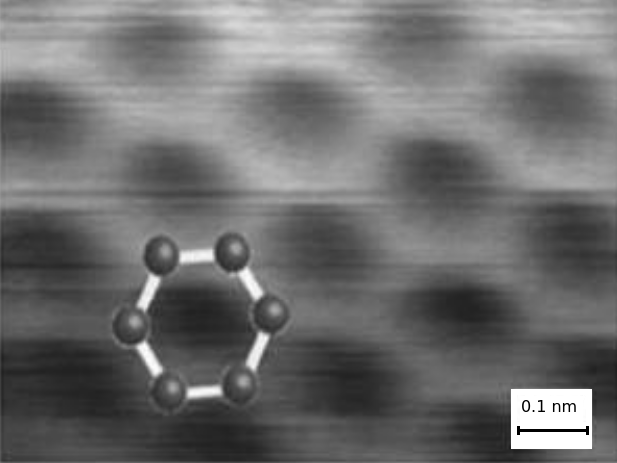
\includegraphics[width=0.8\textwidth]{figs/tem.png}

Transmission electron microscopy of graphene.
\footnote[frame]{\tiny E. Stolyarova, et al. PNAS, 104(22):9209, 2007.}
\end{center}



\end{columns}

\hspace{5mm}

\end{frame}


%%%%%%%%%%%%%%%%%%%%%%%%%%%%%%%%%%%%%%%%%%%%%%%%%%%%%%%%%%%%%%%%%%%%%%%%%%%%%


%%%%%%%%%%%%%%%%%%%%%%%
\subsection{Synthesis}
%%%%%%%%%%%%%%%%%%%%%%%

\begin{frame}

\vspace{-0.2cm}

\noindent\makebox[\linewidth]{\rule{\linewidth}{0.4pt}}

\vspace{-2.0mm}
\begin{center}
{\huge Synthesis of graphene}
\end{center}

\vspace{-6mm}
\noindent\makebox[\linewidth]{\rule{\linewidth}{0.4pt}}

\begin{columns}
\column{0.51\textwidth}
\begin{itemize}

\item Exfoliation\footnote[frame]{\tiny A.K. Geim and K.S. Novoselov. Nature
Materials, 6(3):183-191, 2007. \label{ft:geimNAT07}}

\item Micromechanical cleavage
\footnote[frame]{\tiny R.R. Nair, et al. Science, 320(5881):1308-1308, 2008.
\label{ft:nairSC08}}


\item Reduction of graphite oxide in dimethylformamide
\footnote[frame]{\tiny S. Park, J. et al. Nano letters, 9(4):1593-1597, 2009.}

\item Chemical Vapor Deposition
\footnote[frame]{\tiny E. Rollings, et al. JPCS,
67(9-10):2172-2177, 2006.}

\end{itemize}
\column{0.6\textwidth}
\begin{figure}
\centering
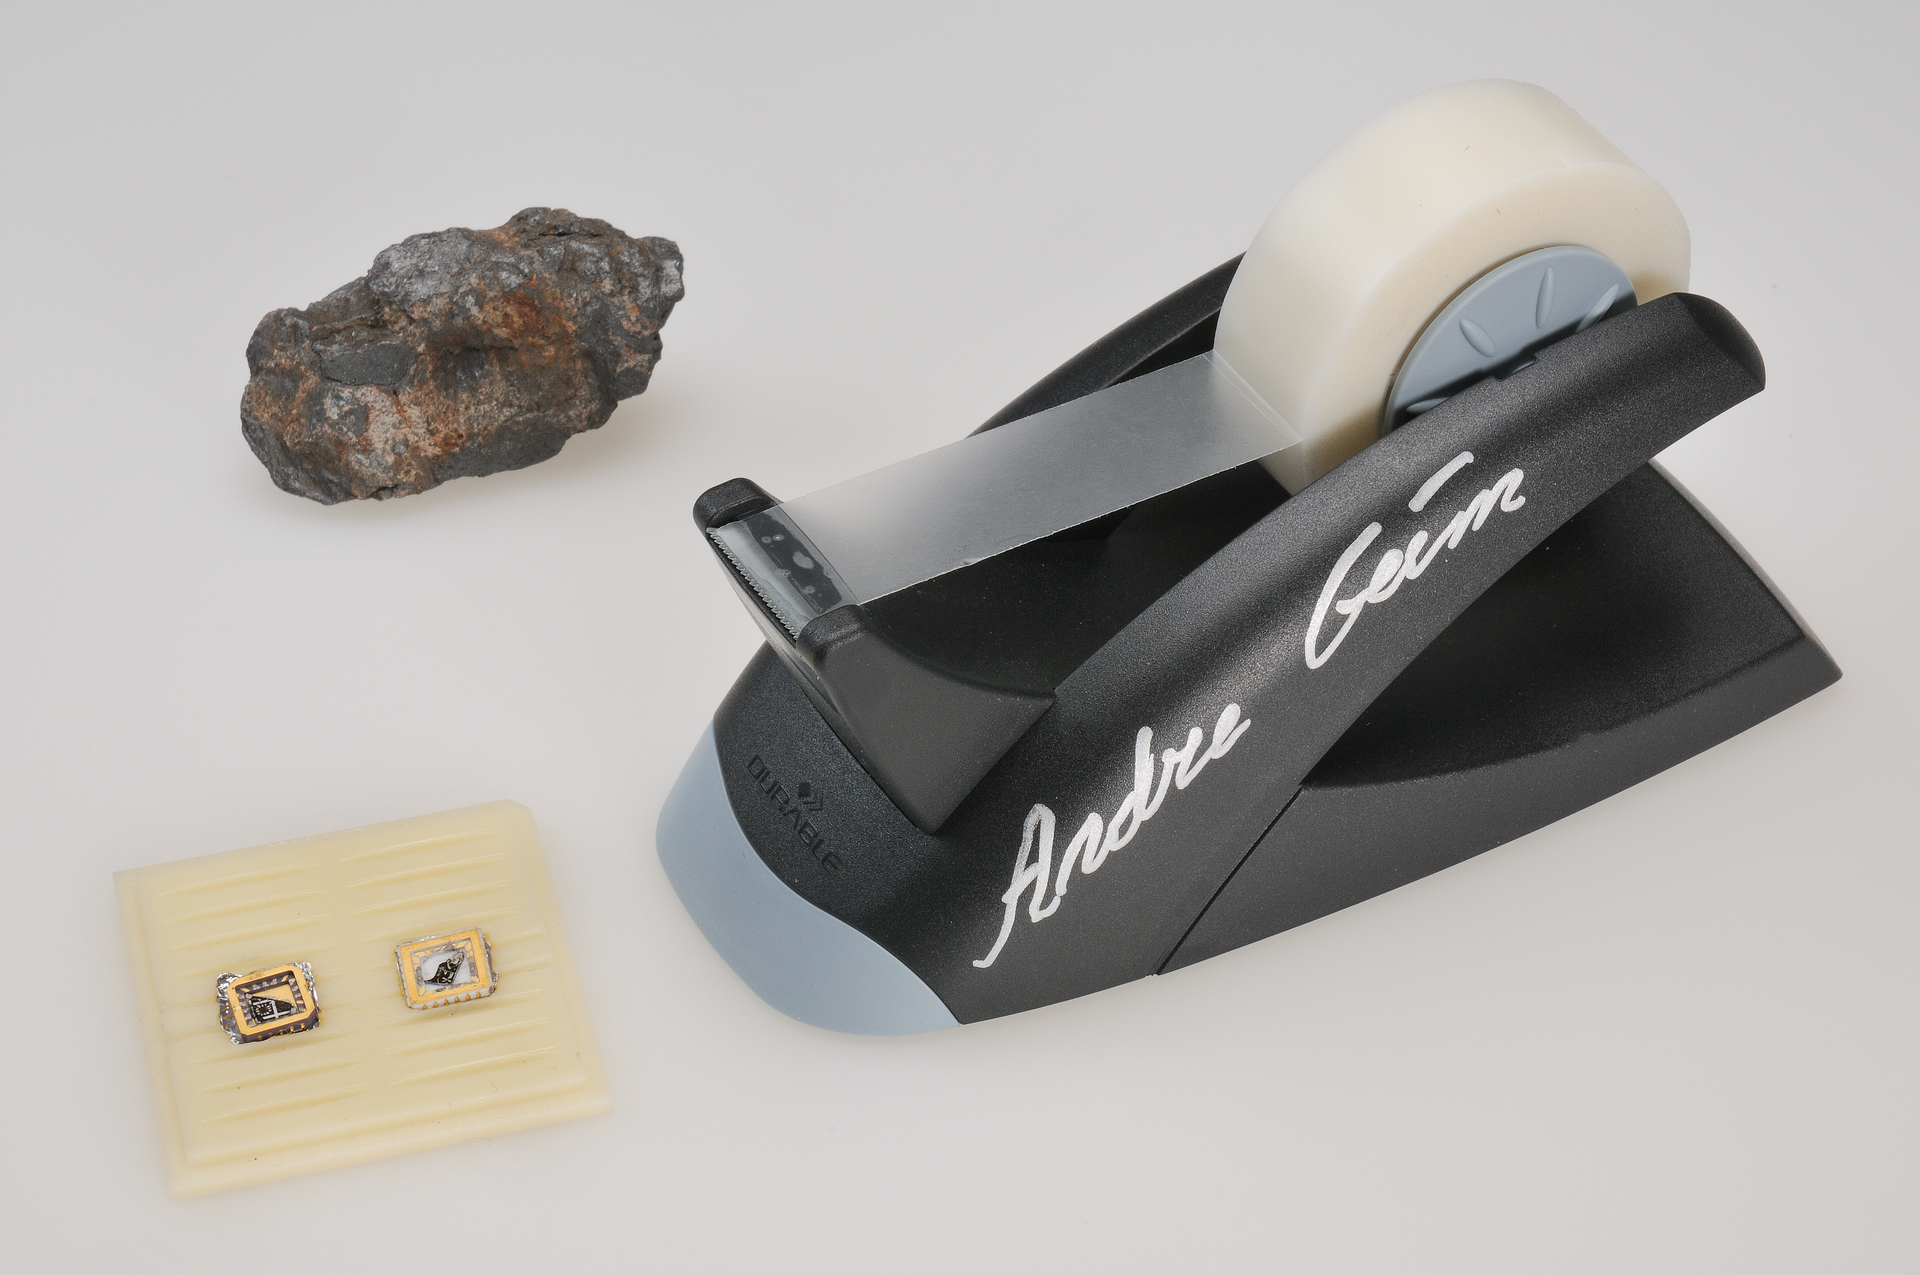
\includegraphics[width=0.75\textwidth]{figs/tools.png}

{\scriptsize Graphite, a graphene transistor, and a tape dispenser donated to
the Nobel Museum.}\footnote[frame]{\tiny By
Gabriel Hildebrand - Nobelmuseet, Public Domain.}
\end{figure}

\end{columns}

\hspace{5mm}

\end{frame}


%%%%%%%%%%%%%%%%%%%%%%%%%%%%%%%%%%%%%%%%%%%%%%%%%%%%%%%%%%%%%%%%%%%%%%%%%%%%%


\begin{frame}

\begin{columns}

\column{0.3\textwidth}

\begin{center}
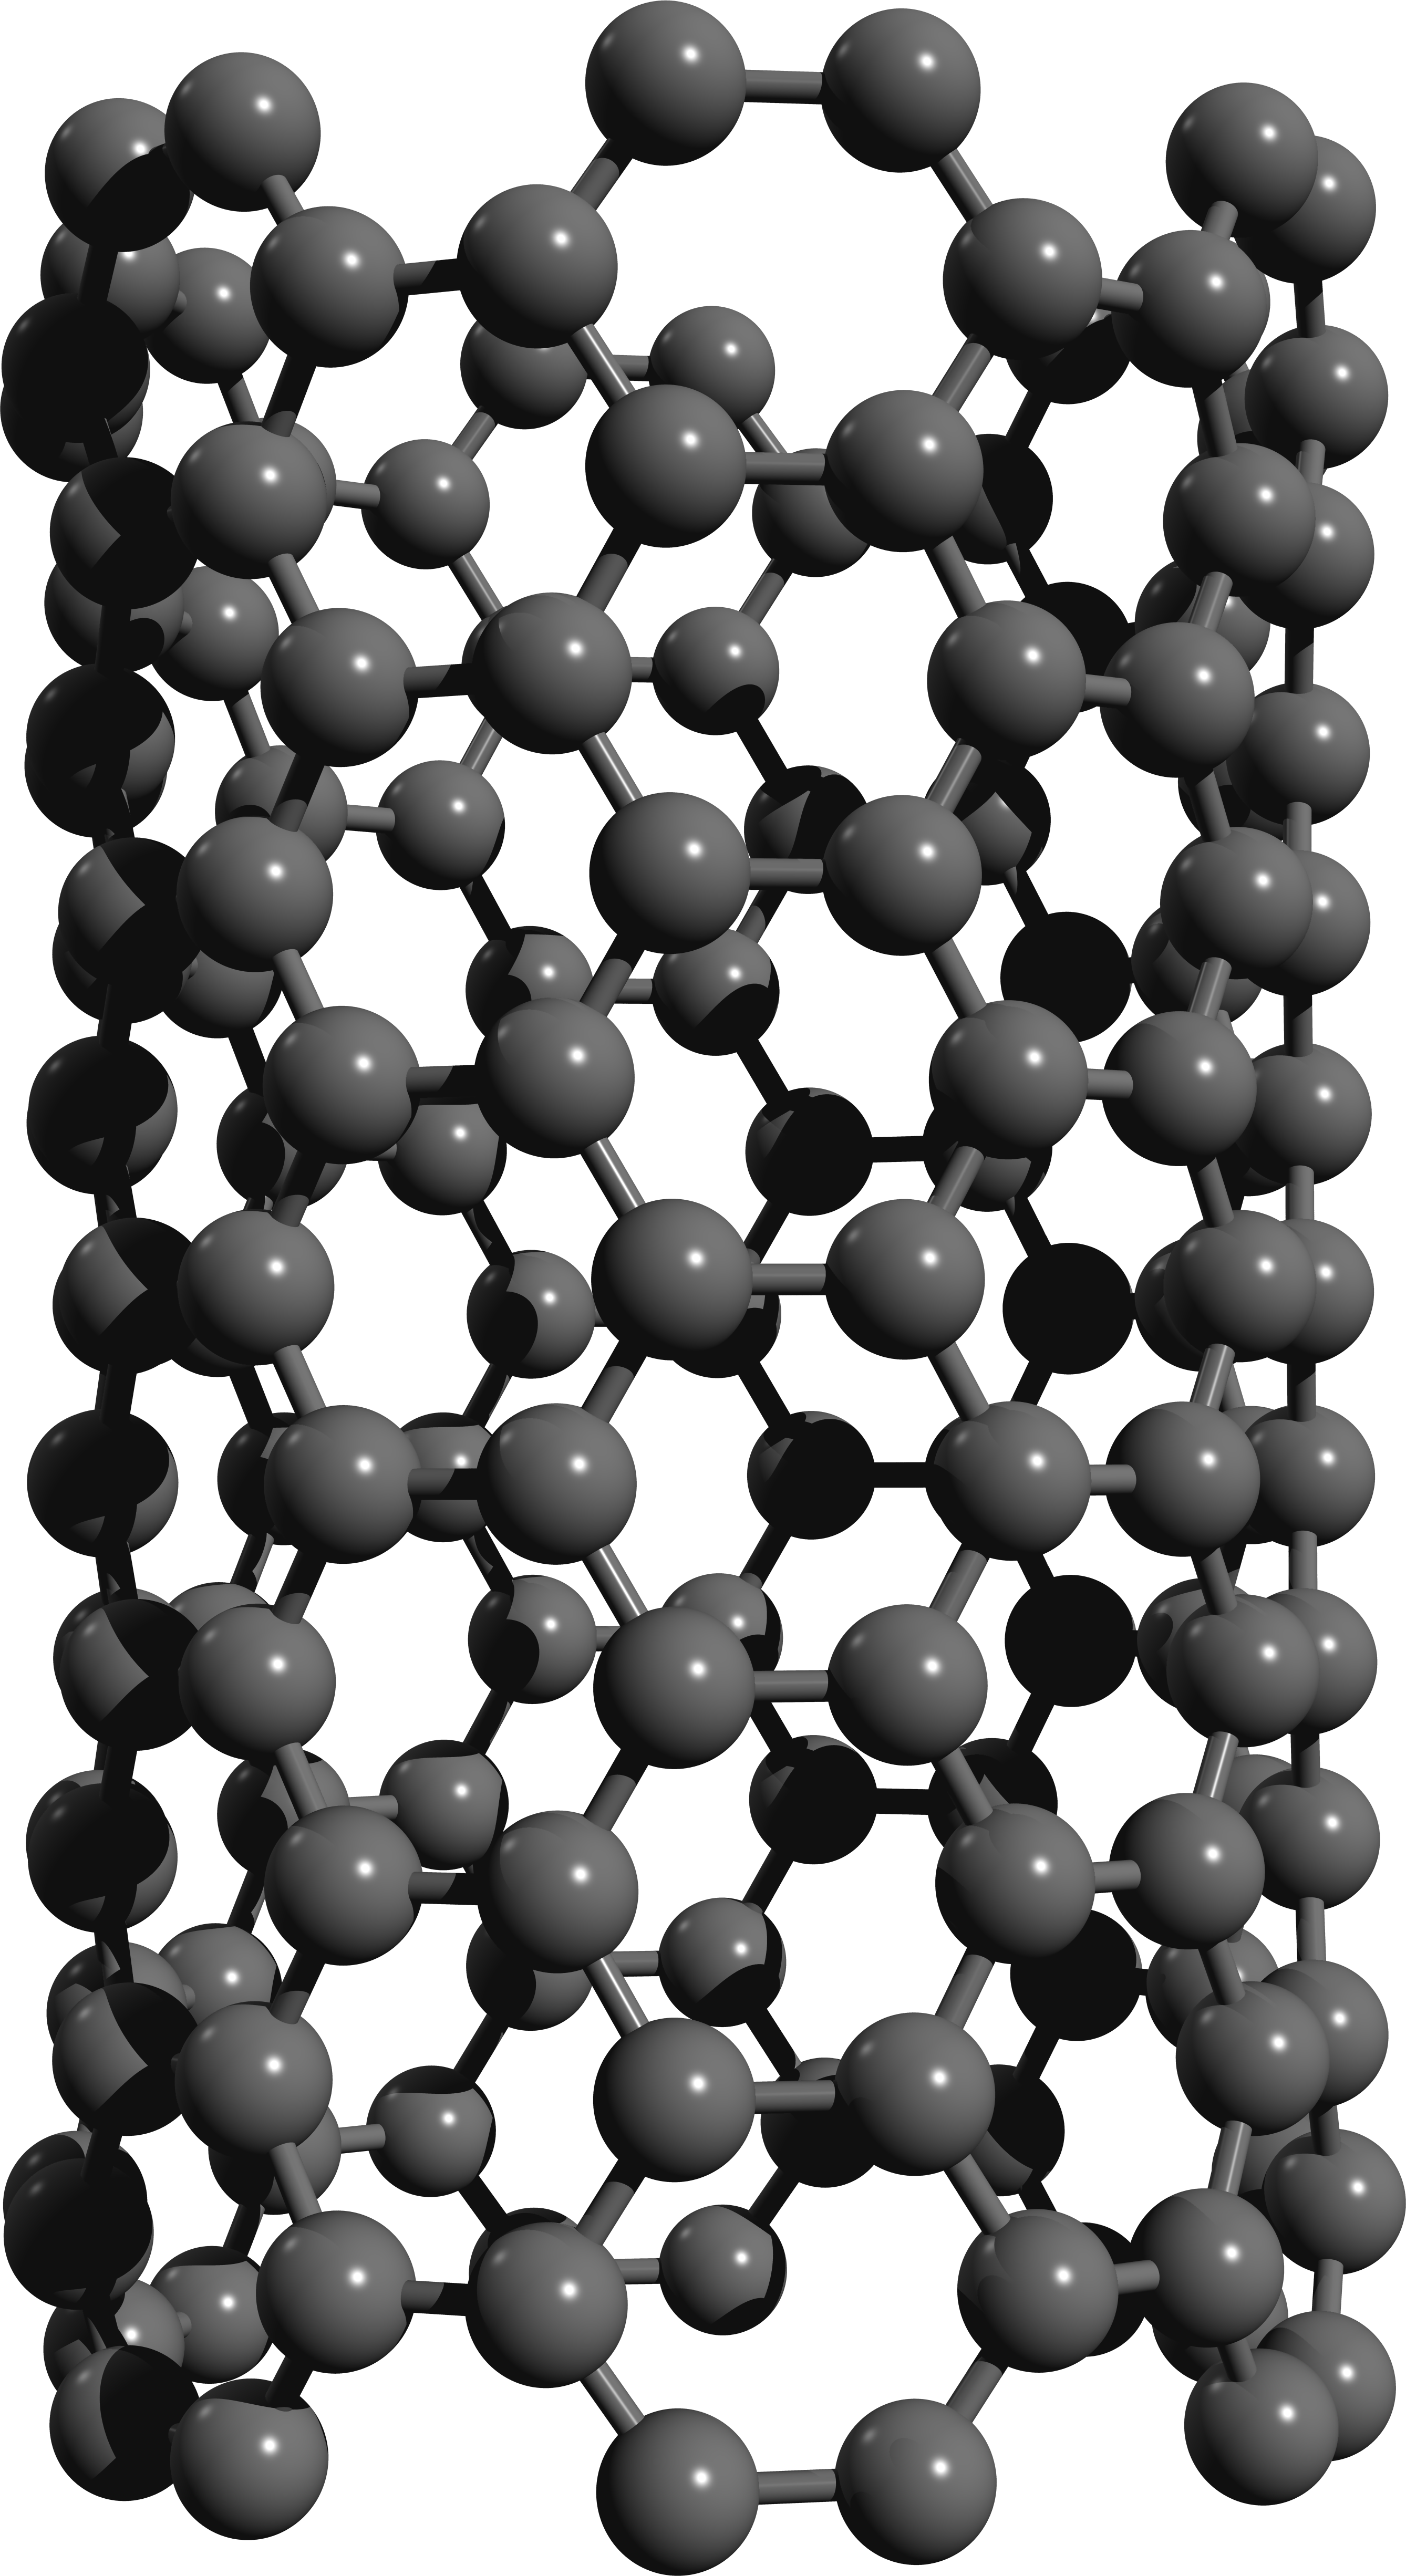
\includegraphics[width=0.9\textwidth]{figs/nanotube2.png}\\

\vspace{3mm}
Carbon nanotube
\end{center}

\column{0.7\textwidth}
\begin{center}
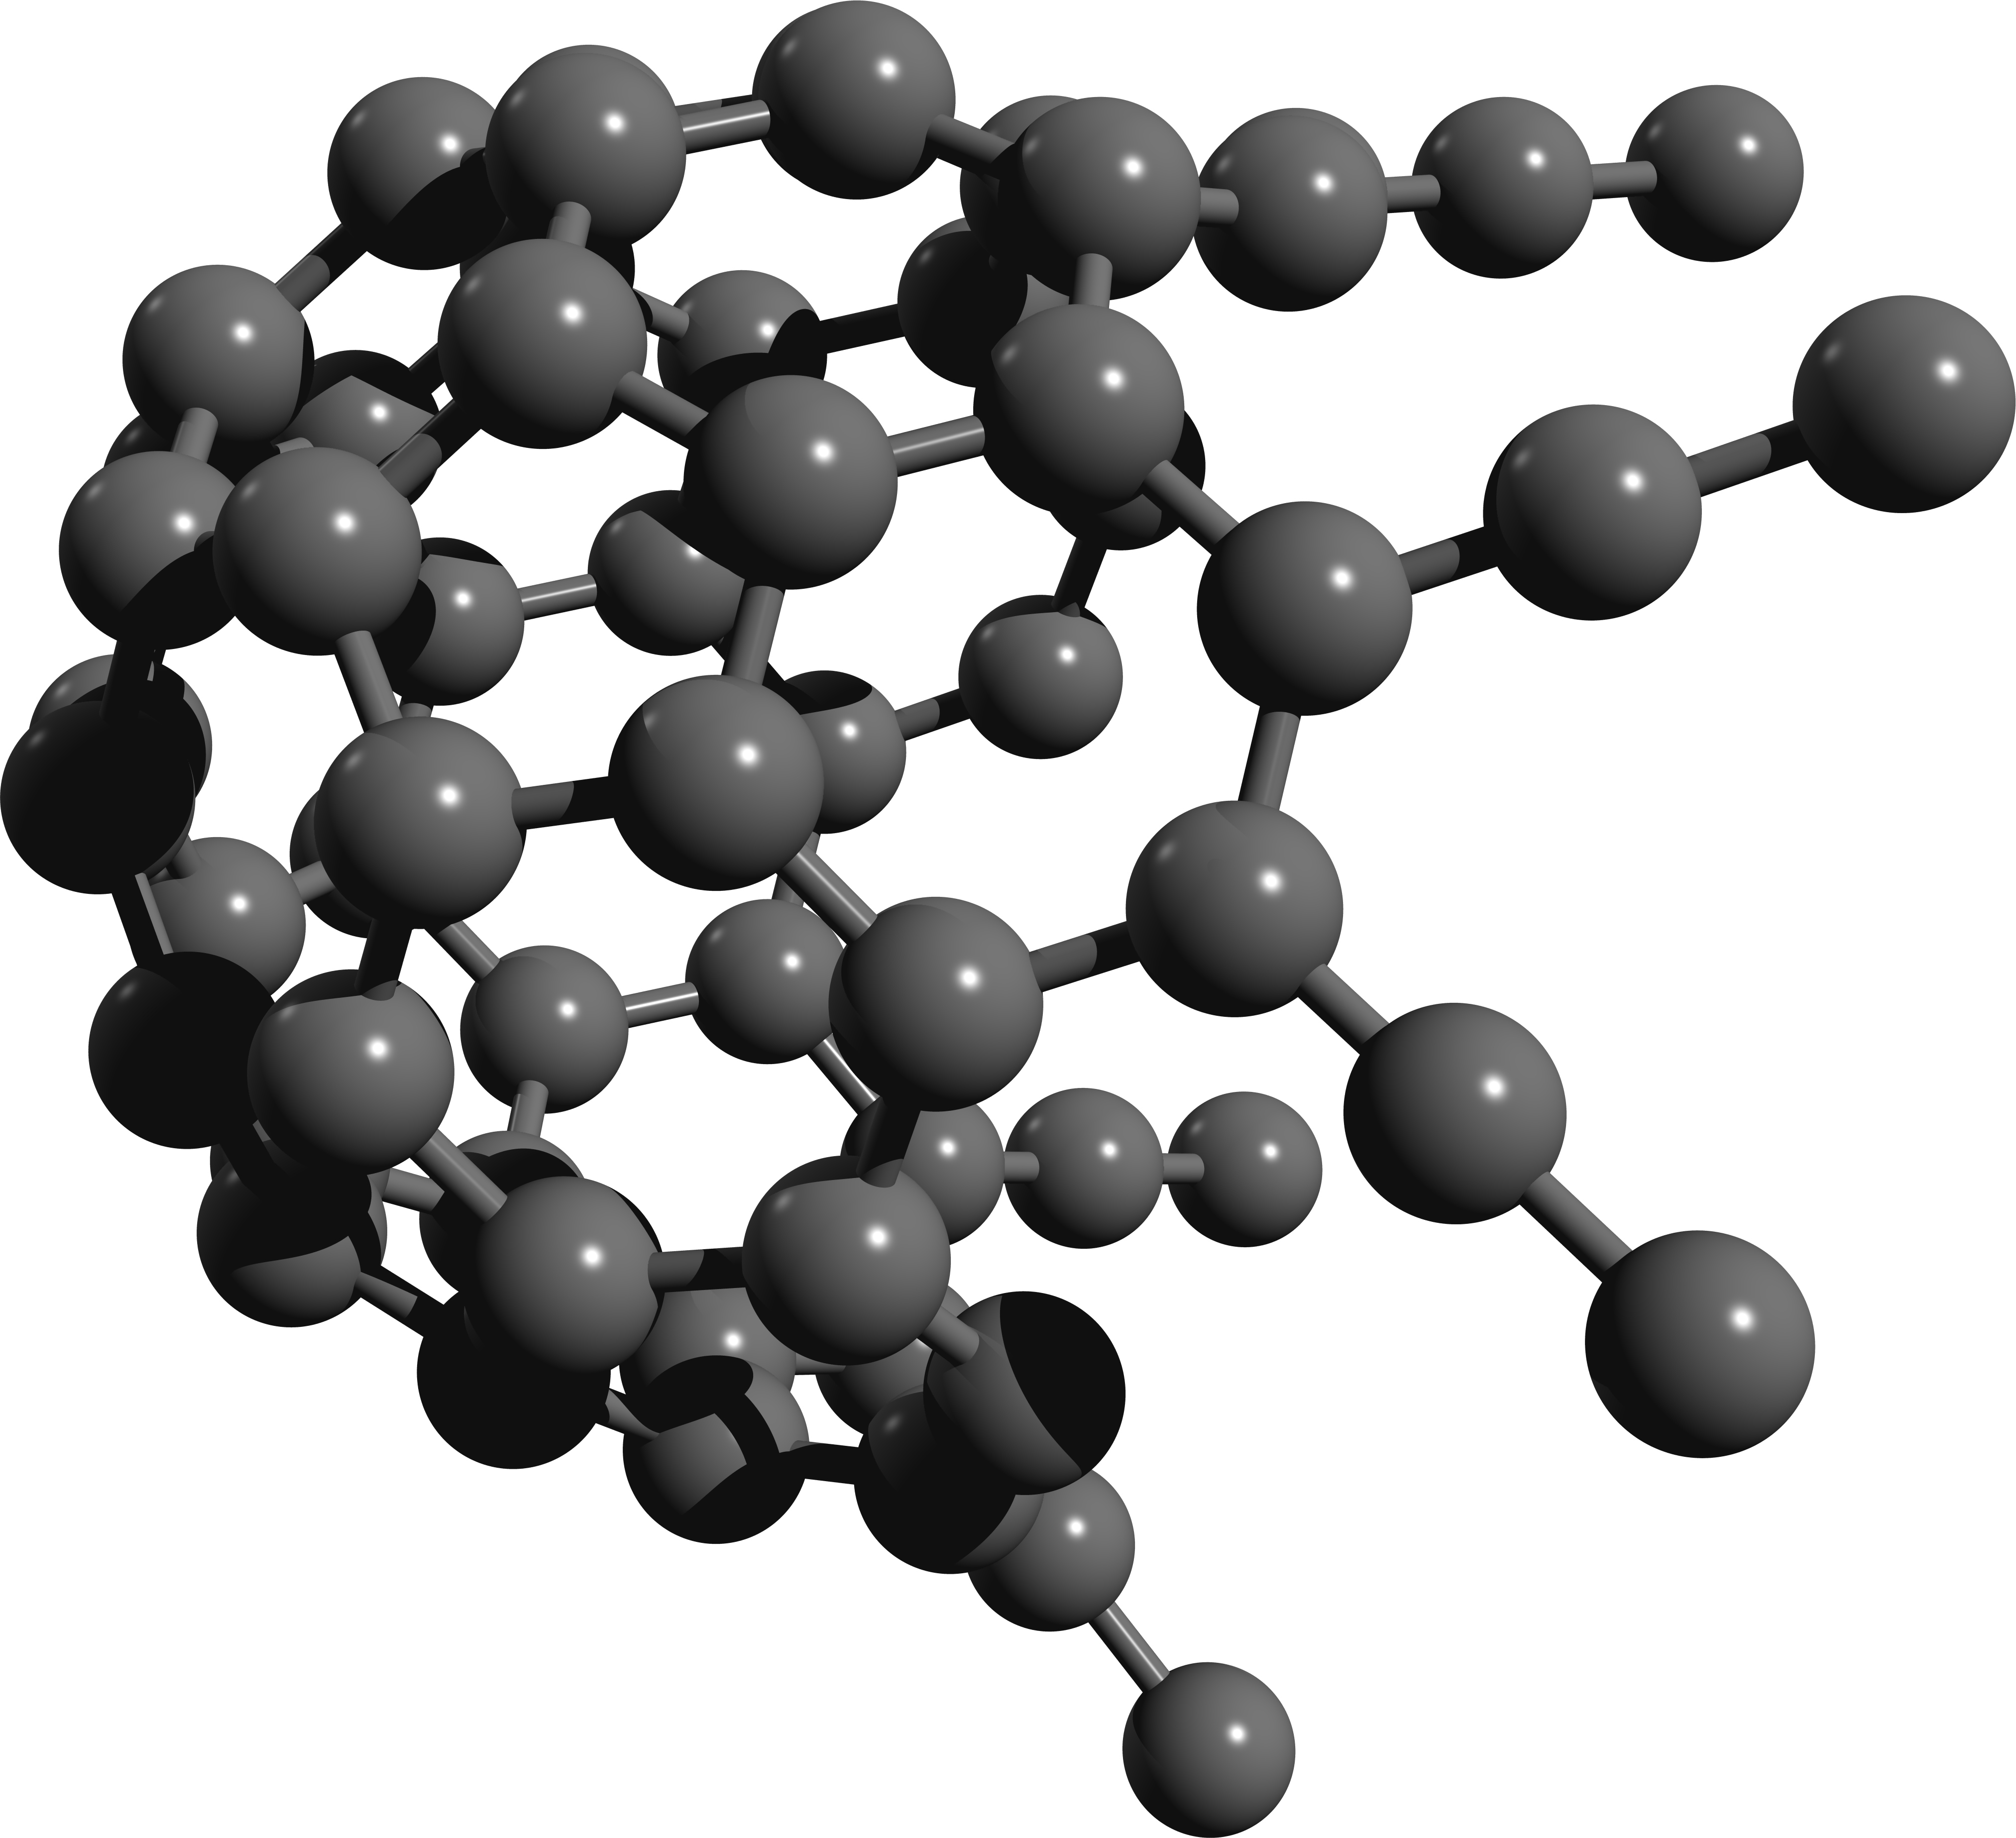
\includegraphics[width=0.35\textwidth]{figs/fullerene2.png} 
\hspace{5mm}
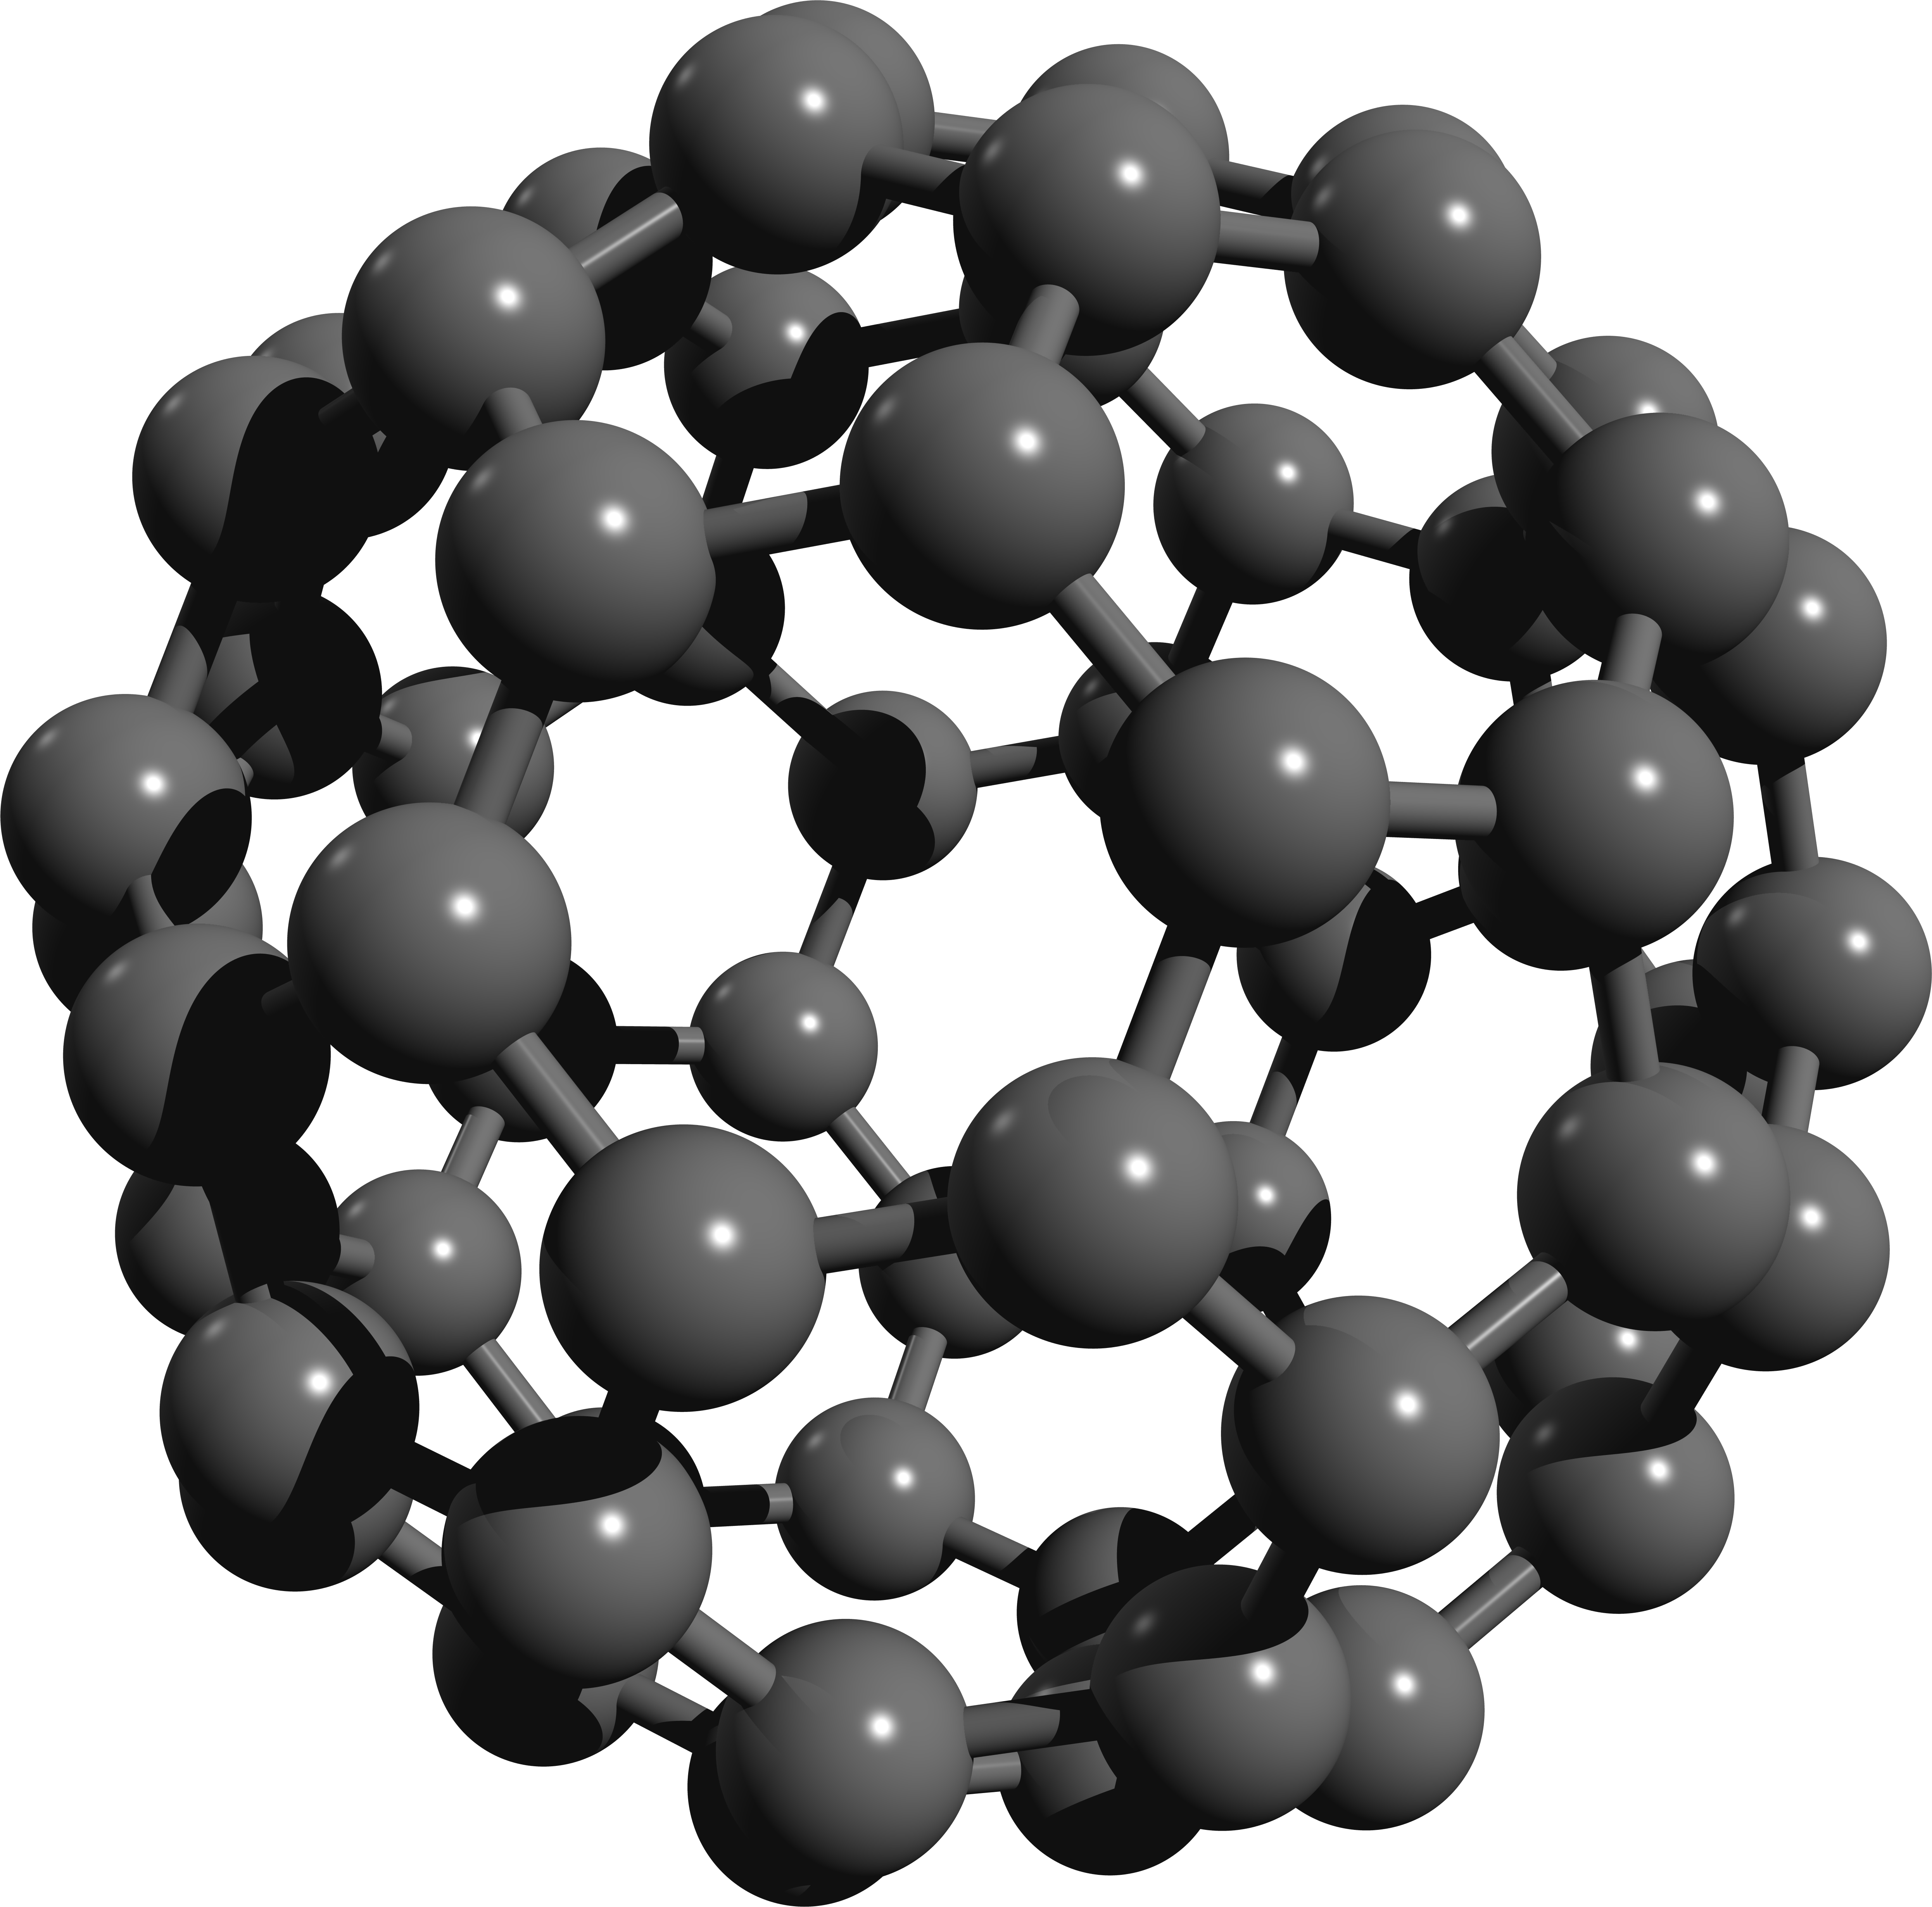
\includegraphics[width=0.35\textwidth]{figs/fullerene1.png}\\
Fullerene

\vspace{5mm}
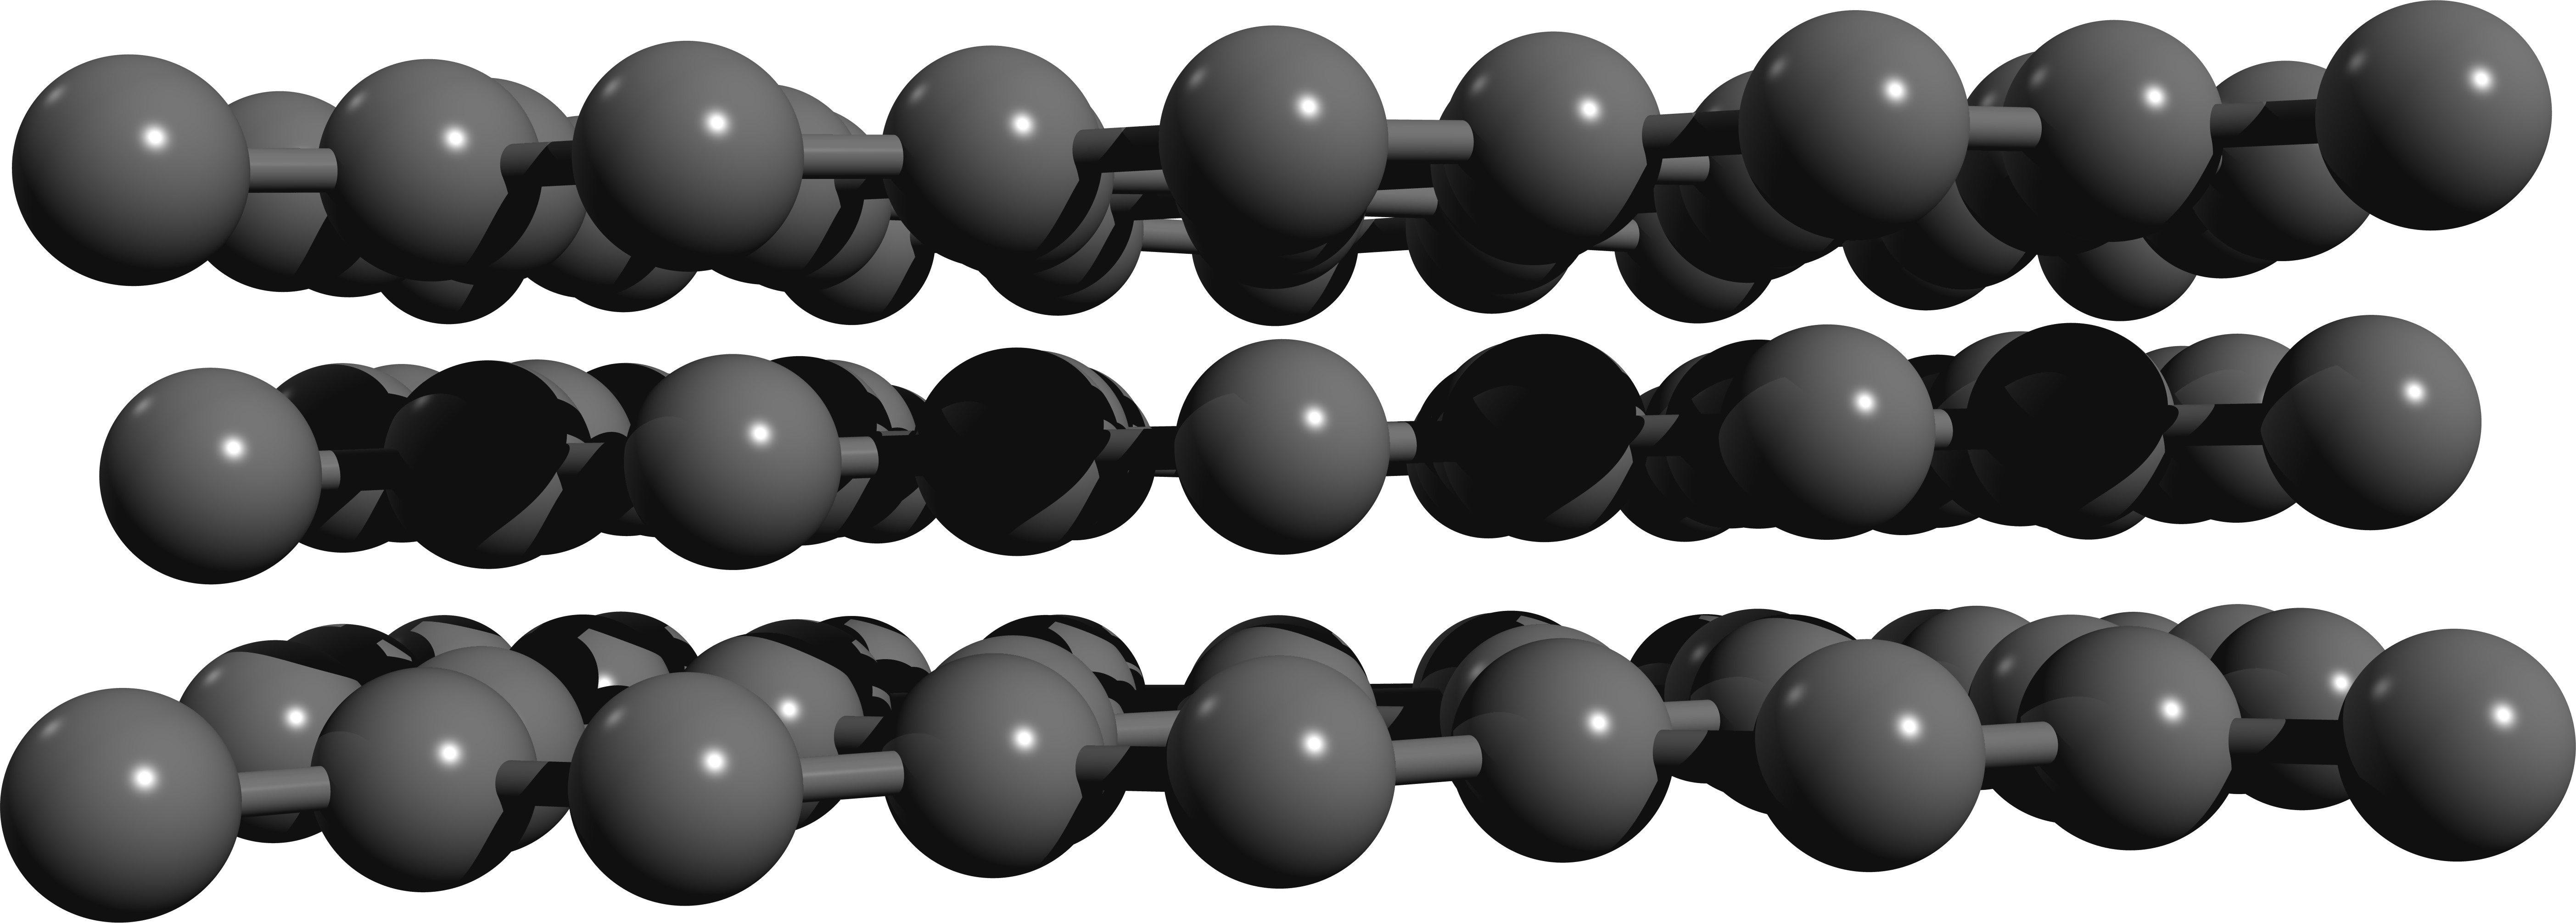
\includegraphics[width=0.35\textwidth]{figs/graphite2.png} 
\vspace{2mm} \hspace{5mm}
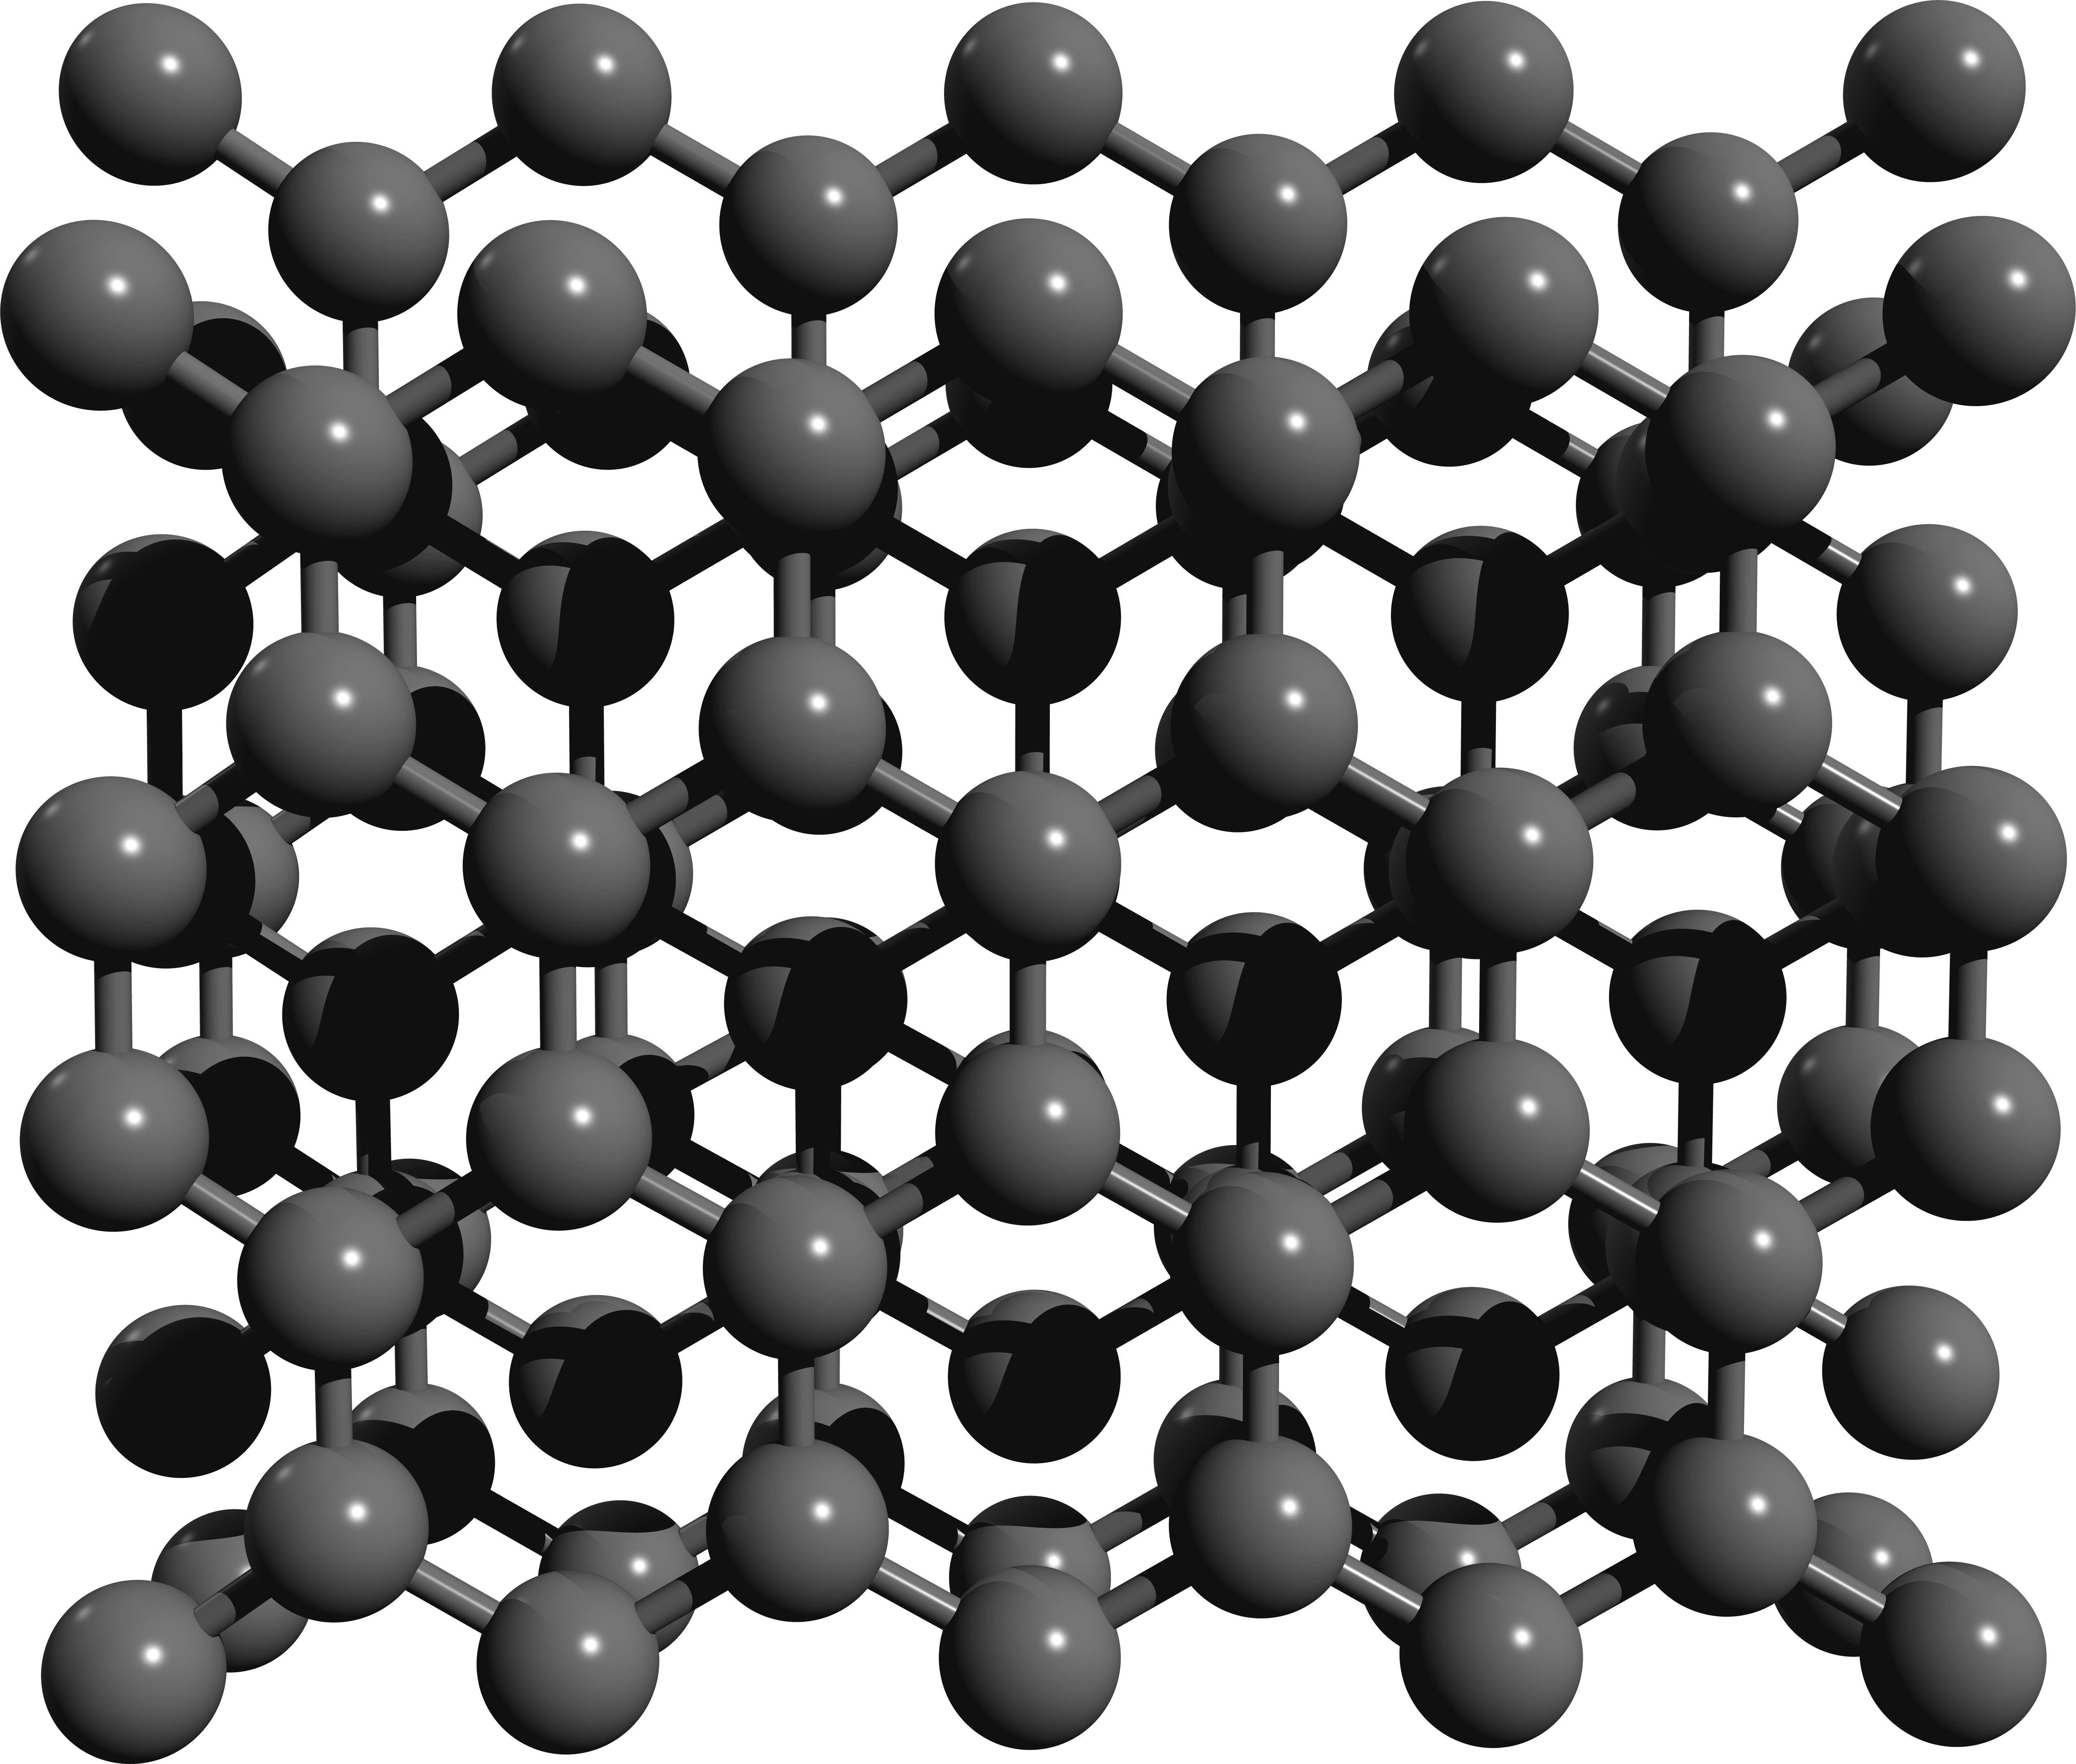
\includegraphics[width=0.35\textwidth]{figs/graphite1.png}\\
Graphite

\end{center}

\end{columns}

\vspace{3mm}
\begin{center}
{\huge Structures obtained from graphene}
\end{center}

\end{frame}

%%%%%%%%%%%%%%%%%%%%%%%%%%%%%%%%%%%%%%%%%%%%%%%%%%%%%%%%%%%%%%%%%%%%%%%%%%%%%


%%%%%%%%%%%%%%%%%%%%%%%
\subsection{Electronic properties}
%%%%%%%%%%%%%%%%%%%%%%%

\begin{frame}
\vspace{-0.3cm}

\noindent\makebox[\linewidth]{\rule{\linewidth}{0.4pt}}

\vspace{-2.0mm}
\begin{center}
{\huge Electronic properties of graphene}
\end{center}

\vspace{-6mm}
\noindent\makebox[\linewidth]{\rule{\linewidth}{0.4pt}}

\vfill

\begin{columns}
\column{0.5\textwidth}
\begin{itemize}

\item Quantum Hall effect at room temperature\textsuperscript{1}

\item Excellent electrical current conduction
\footnote[frame]{\tiny A.K. Geim and K.S. Novoselov. Nature
Materials, 6(3):183-191, 2007.}

% \item Dirac Cones\textsuperscript{ 2}

\item Transparent to visible light
\footnote[frame]{\tiny R.R. Nair, et al. Science, 320(5881):1308-1308, 2008.}

\item Tunable bandgap
\footnote[frame]{\tiny M.Y. Han, et. al. Physical Review Letters,
98(20):206805, 2007}



\end{itemize}
\column{0.5\textwidth}
\begin{figure}
\centering
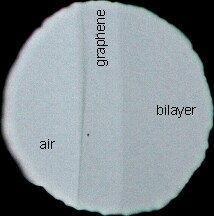
\includegraphics[width=0.65\textwidth]{figs/trasparency.jpg}

Photograph of graphene \\
in transmitted light.
\footnote[frame]{\tiny By Rahul Nair - Manchester group.}
\end{figure}
\end{columns}

\hspace{5mm}
\end{frame}

%%%%%%%%%%%%%%%%%%%%%%%%%%%%%%%%%%%%%%%%%%%%%%%%%%%%%%%%%%%%%%%%%%%%%%%%%%%%%

\begin{frame}

\begin{columns}

\column{0.4\textwidth}

\begin{itemize}
\item Tunable bandgap by:
\noindent
\begin{itemize}

\item[-] changing sheet size
\footnote[frame]{\tiny C. Feng et al. 2009. Jour. of Chem. Phis. 131:194702,
2009. \label{ft:fengJCP09}}

\item[-] changing number of sheets and stacking\textsuperscript{
\ref{ft:fengJCP09}}

\item[-] applying an electric field
\footnote[frame]{\tiny Y. Zhang et al. Nature, 459(7248):820-823, 2009.
\label{ft:ahangNAT09}}

\item[-] doping
\footnote[frame]{\tiny T. Ohta et al. Science, 313(5789):951-954, 2006.
\label{ft:ohtaSC06}}

\item[-] hydrogenation
\footnote[frame]{\tiny D.C. Elias et al. Science, 323(5914):610-613, 2009.
\label{ft:eliasSC09}}

\end{itemize}
\end{itemize}

\column{0.7\textwidth}


\begin{center}
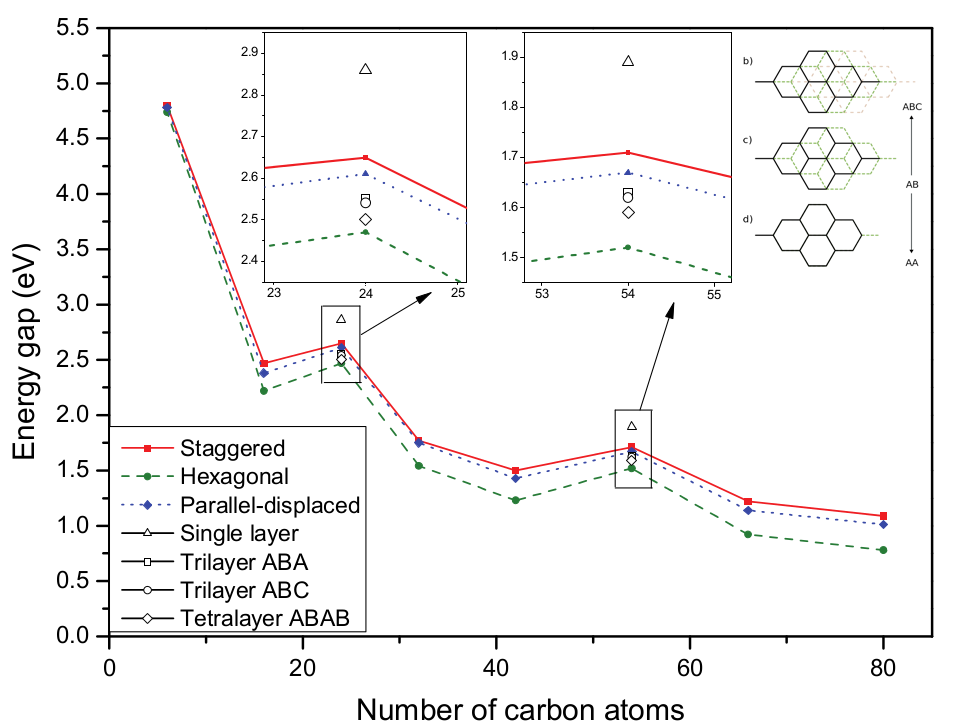
\includegraphics[width=0.9\textwidth]{figs/gap.png}

{\footnotesize Variation of the energy gap with the size of graphene sheet
model.\textsuperscript{ \ref{ft:fengJCP09}}}
\end{center}
    
\end{columns}
\end{frame}


%%%%%%%%%%%%%%%%%%%%%%%%%%%%%%%%%%%%%%%%%%%%%%%%%%%%%%%%%%%%%%%%%%%%%%%%%%%%%


%%%%%%%%%%%%%%%%%%%%%%%
\subsection{Functionalization}
%%%%%%%%%%%%%%%%%%%%%%%

\begin{frame}

\begin{columns}

\column{0.5\textwidth}

\begin{center}
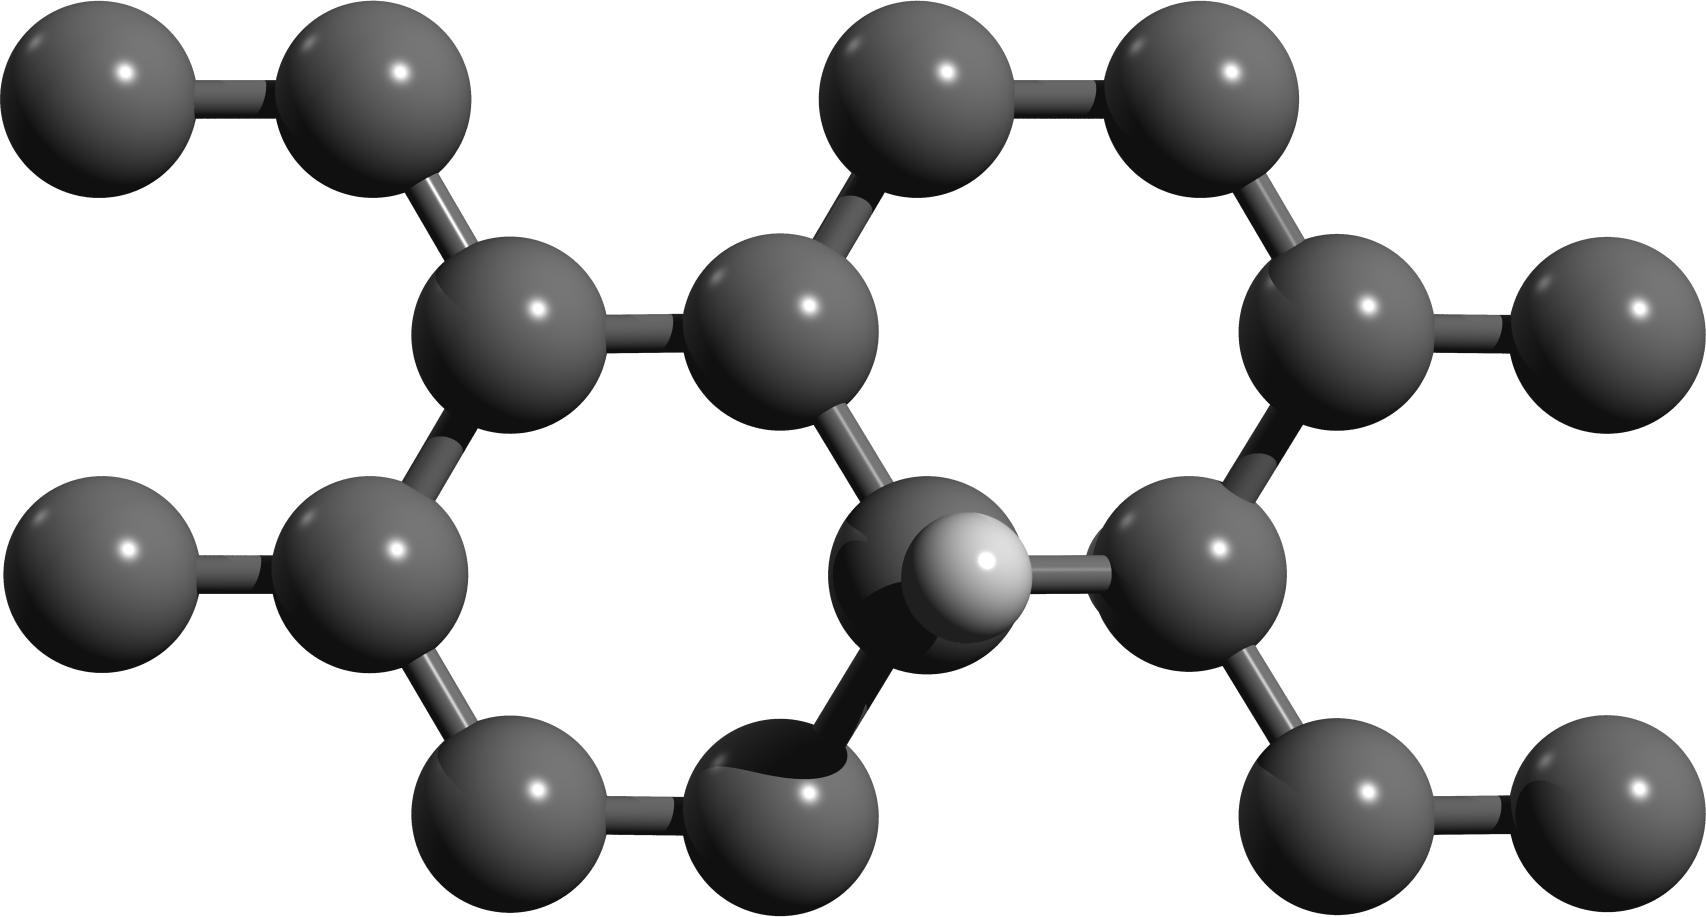
\includegraphics[width=0.8\textwidth]{figs/row.png}\\
% {\small 12.5\% of hydrogenation}

\vspace{7mm}
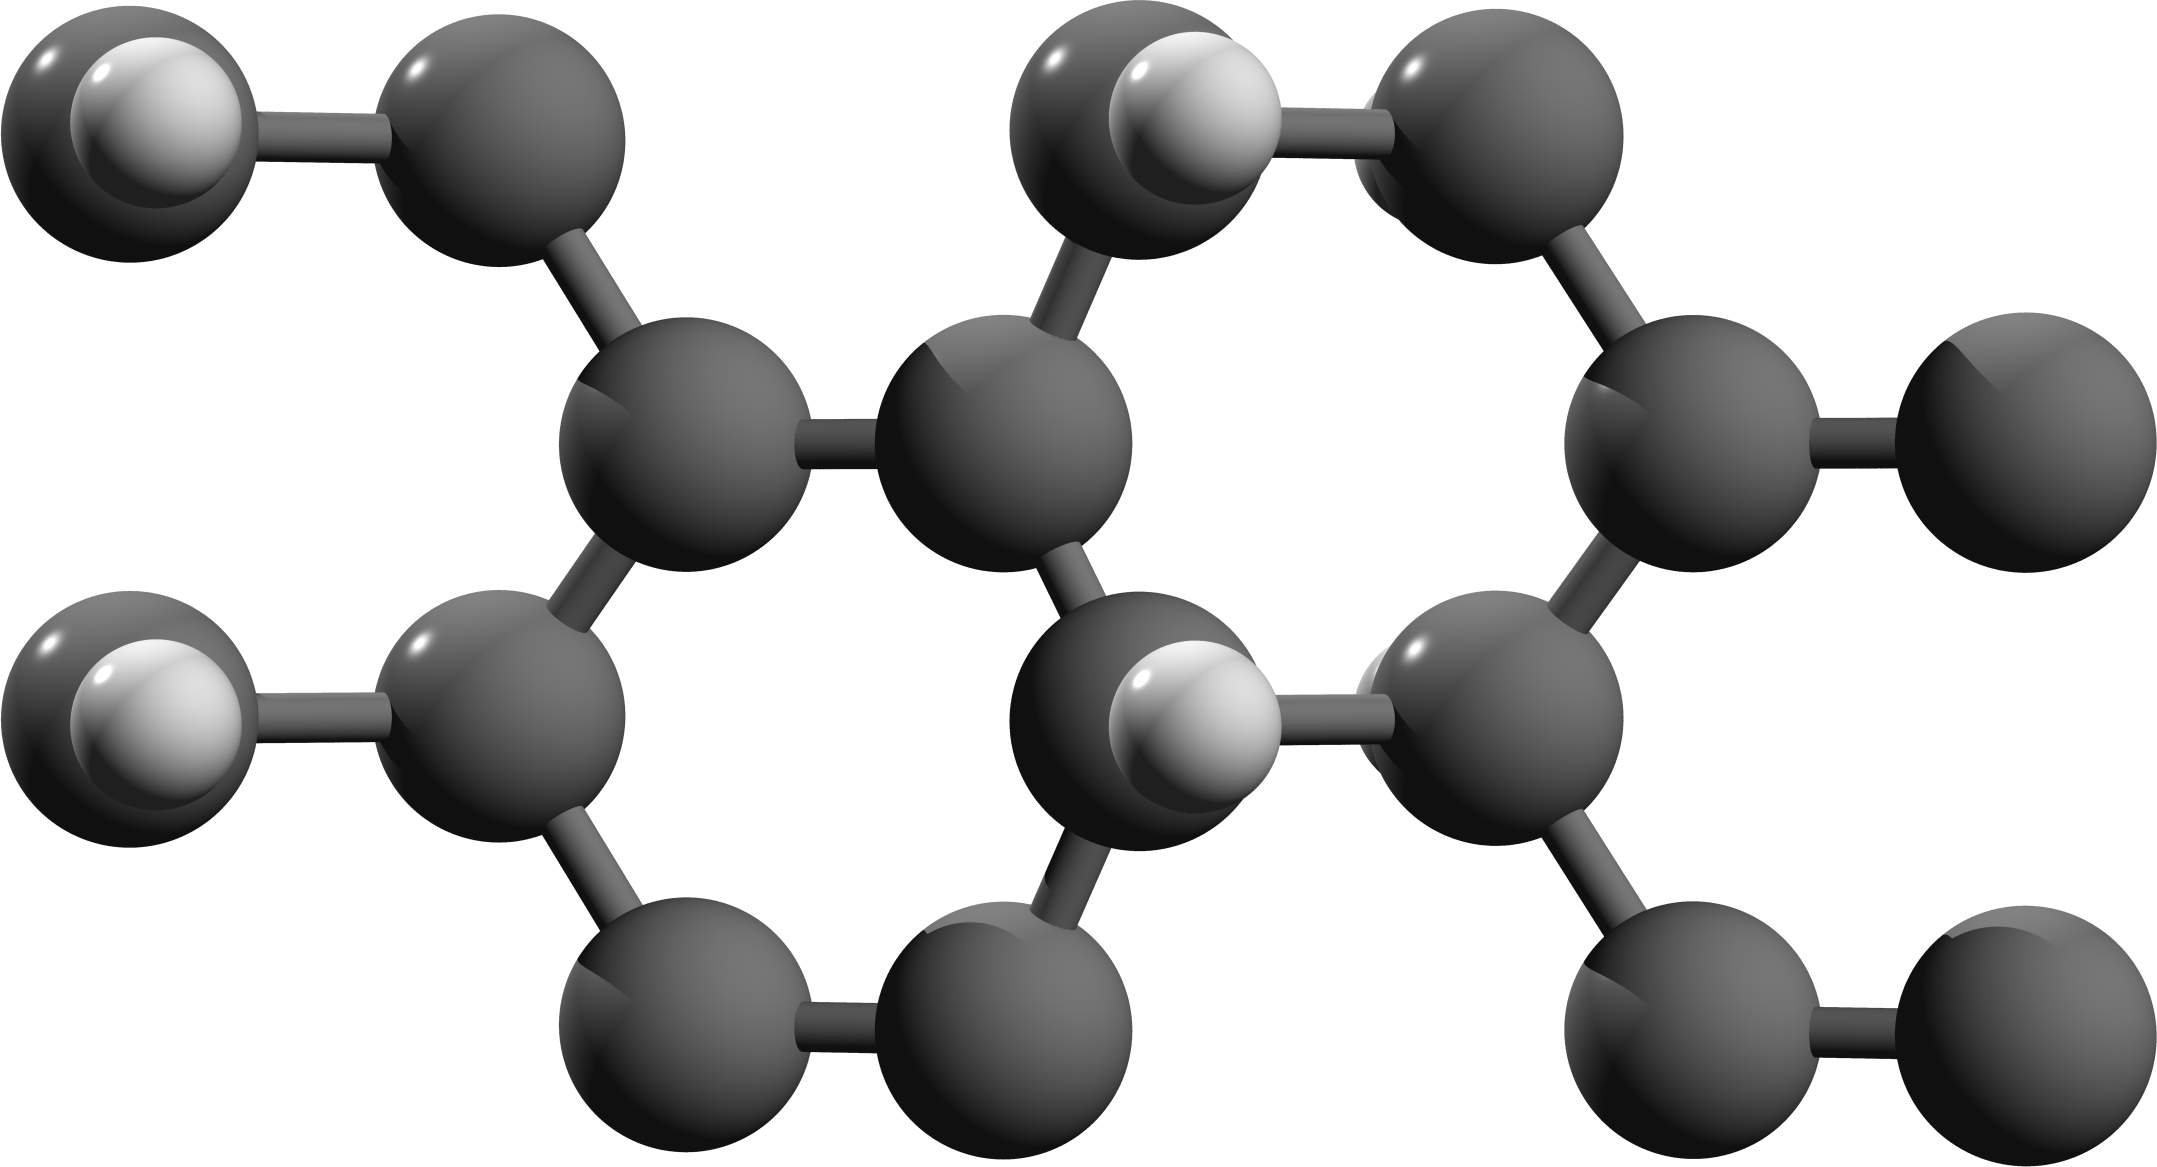
\includegraphics[width=0.8\textwidth]{figs/alt1.png}\\
% {\small 50\% of hydrogenation}


\vspace{5mm}
\end{center}

\column{0.5\textwidth}

\centering
\begin{center}
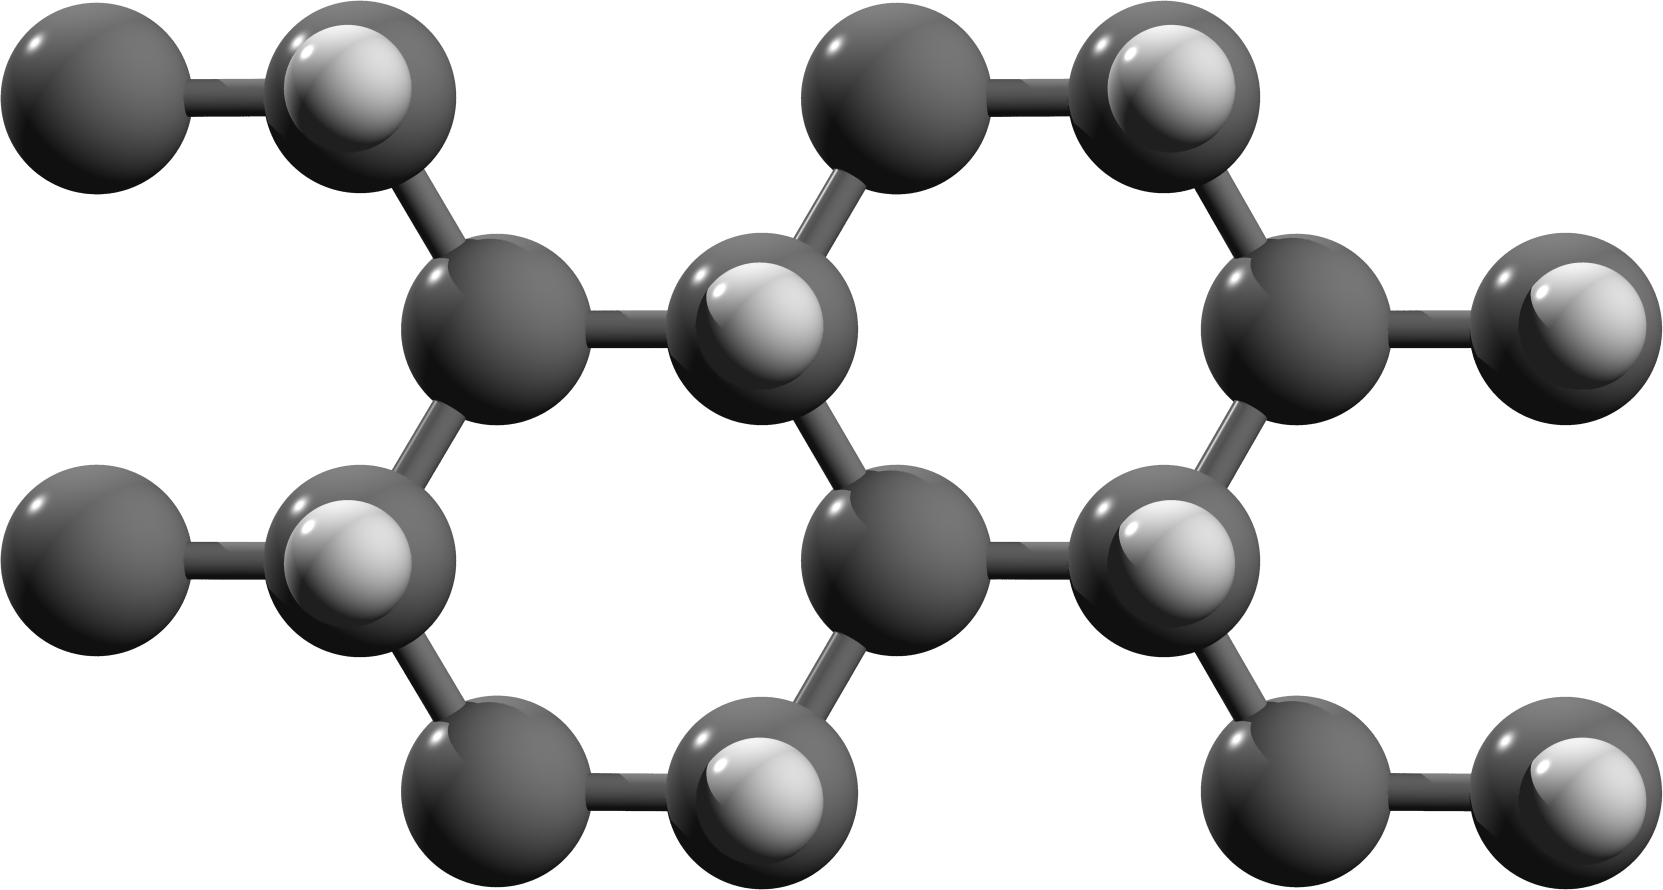
\includegraphics[width=0.8\textwidth]{figs/up1.png}\\
% {\small 50\% of hydrogenation}

\vspace{7mm}
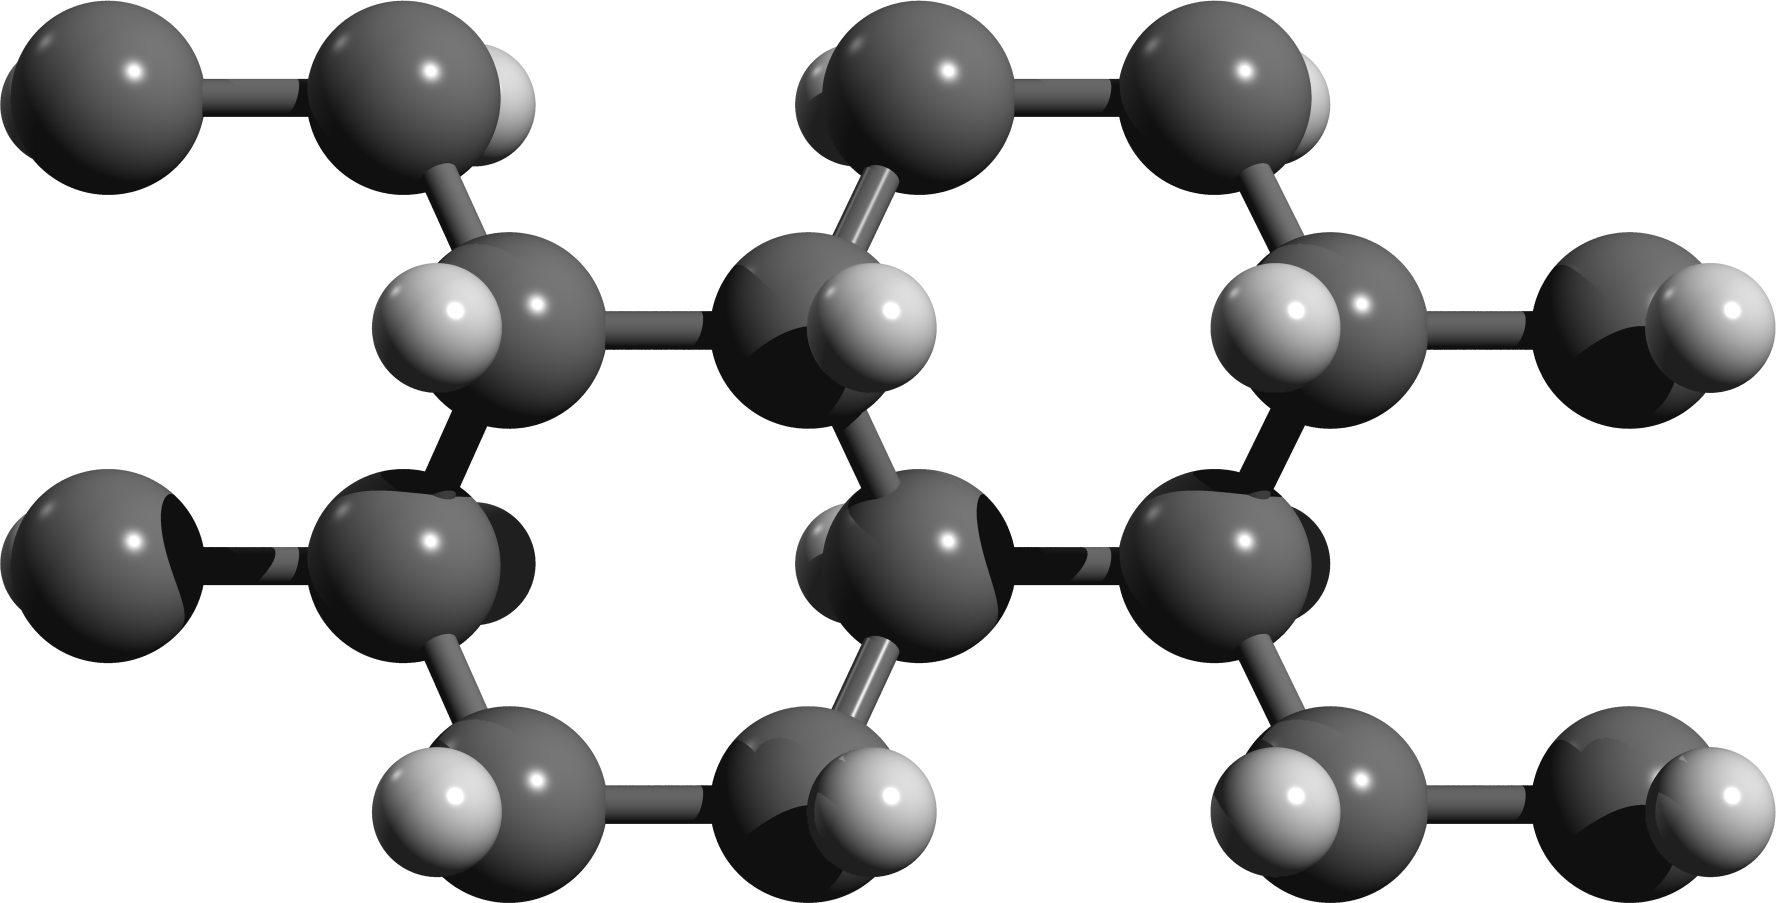
\includegraphics[width=0.8\textwidth]{figs/boat.png}\\
% {\small 100\% of hydrogenation}

\vspace{3mm}
\end{center}

\end{columns}

\begin{center}

{\huge Functionalization by hydrogenation}
\end{center}
\end{frame}

%%%%%%%%%%%%%%%%%%%%%%%%%%%%%%%%%%%%%%%%%%%%%%%%%%%%%%%%%%%%%%%%%%%%%%%%%%%%%


%%%%%%%%%%%%%%%%%%%%%%%%%%%%%%%%%%%%%%%%%%%%%%%%%%%%%%%%%%%%%%%%%%%%%%%%%%%%%
\section{The structures}
%%%%%%%%%%%%%%%%%%%%%%%%%%%%%%%%%%%%%%%%%%%%%%%%%%%%%%%%%%%%%%%%%%%%%%%%%%%%%



%%%%%%%%%%%%%%%%%%%%%%%
\subsection{Centrosymmetric Materials}
%%%%%%%%%%%%%%%%%%%%%%%

\begin{frame}

\vspace{-0.2cm}

\noindent\makebox[\linewidth]{\rule{\linewidth}{0.4pt}}

\vspace{-2.0mm}
\begin{center}
{\large Centrosymmetric Materials}
\end{center}

\vspace{-5mm}
\noindent\makebox[\linewidth]{\rule{\linewidth}{0.4pt}}

\begin{center}
A centrosymmetric system presents inversion of symmetry, such
that a point $p(a, b, c)$ corresponds a point $p'(-a, -b, -c)$.
\end{center}


\begin{figure}[h!]
\begin{tikzpicture}

\node[anchor=south west,inner sep=0] at (0.2,-0.3) 
{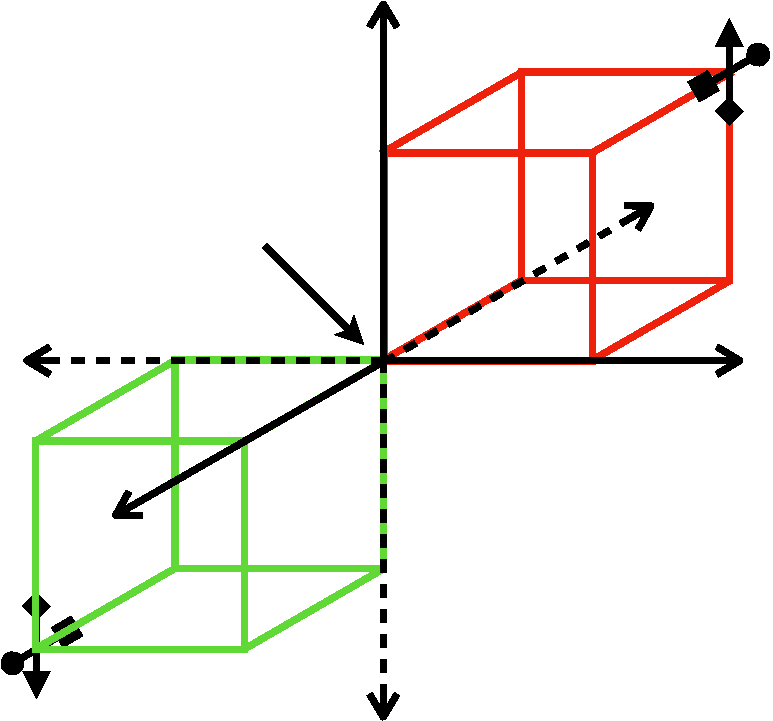
\includegraphics[width=0.5\textwidth]{figs/inversion.pdf}};
\draw [] (5.40, 2.20) node [right] {$x$};
\draw [] (2.65, 5.00) node [right] {$y$};
\draw [] (0.50, 1.00) node [right] {$z$};
\draw [] (5.40, 4.80) node [right] {$p(a,b,c)$};
\draw [](-2.35, 0.00) node [right] {$p'(-a,-b,-c)$};
\draw [](-0.60, 3.20) node [right] {\rmfamily inversion point};

\end{tikzpicture}
\end{figure}


\end{frame}


%%%%%%%%%%%%%%%%%%%%%%%%%%%%%%%%%%%%%%%%%%%%%%%%%%%%%%%%%%%%%%%%%%%%%%%%%%%%%


%%%%%%%%%%%%%%%%%%%%%%%
\subsection{Alt structure}
%%%%%%%%%%%%%%%%%%%%%%%


\begin{frame}

\vspace{-3mm}
\begin{columns}

\column{0.7\textwidth}
\flushright
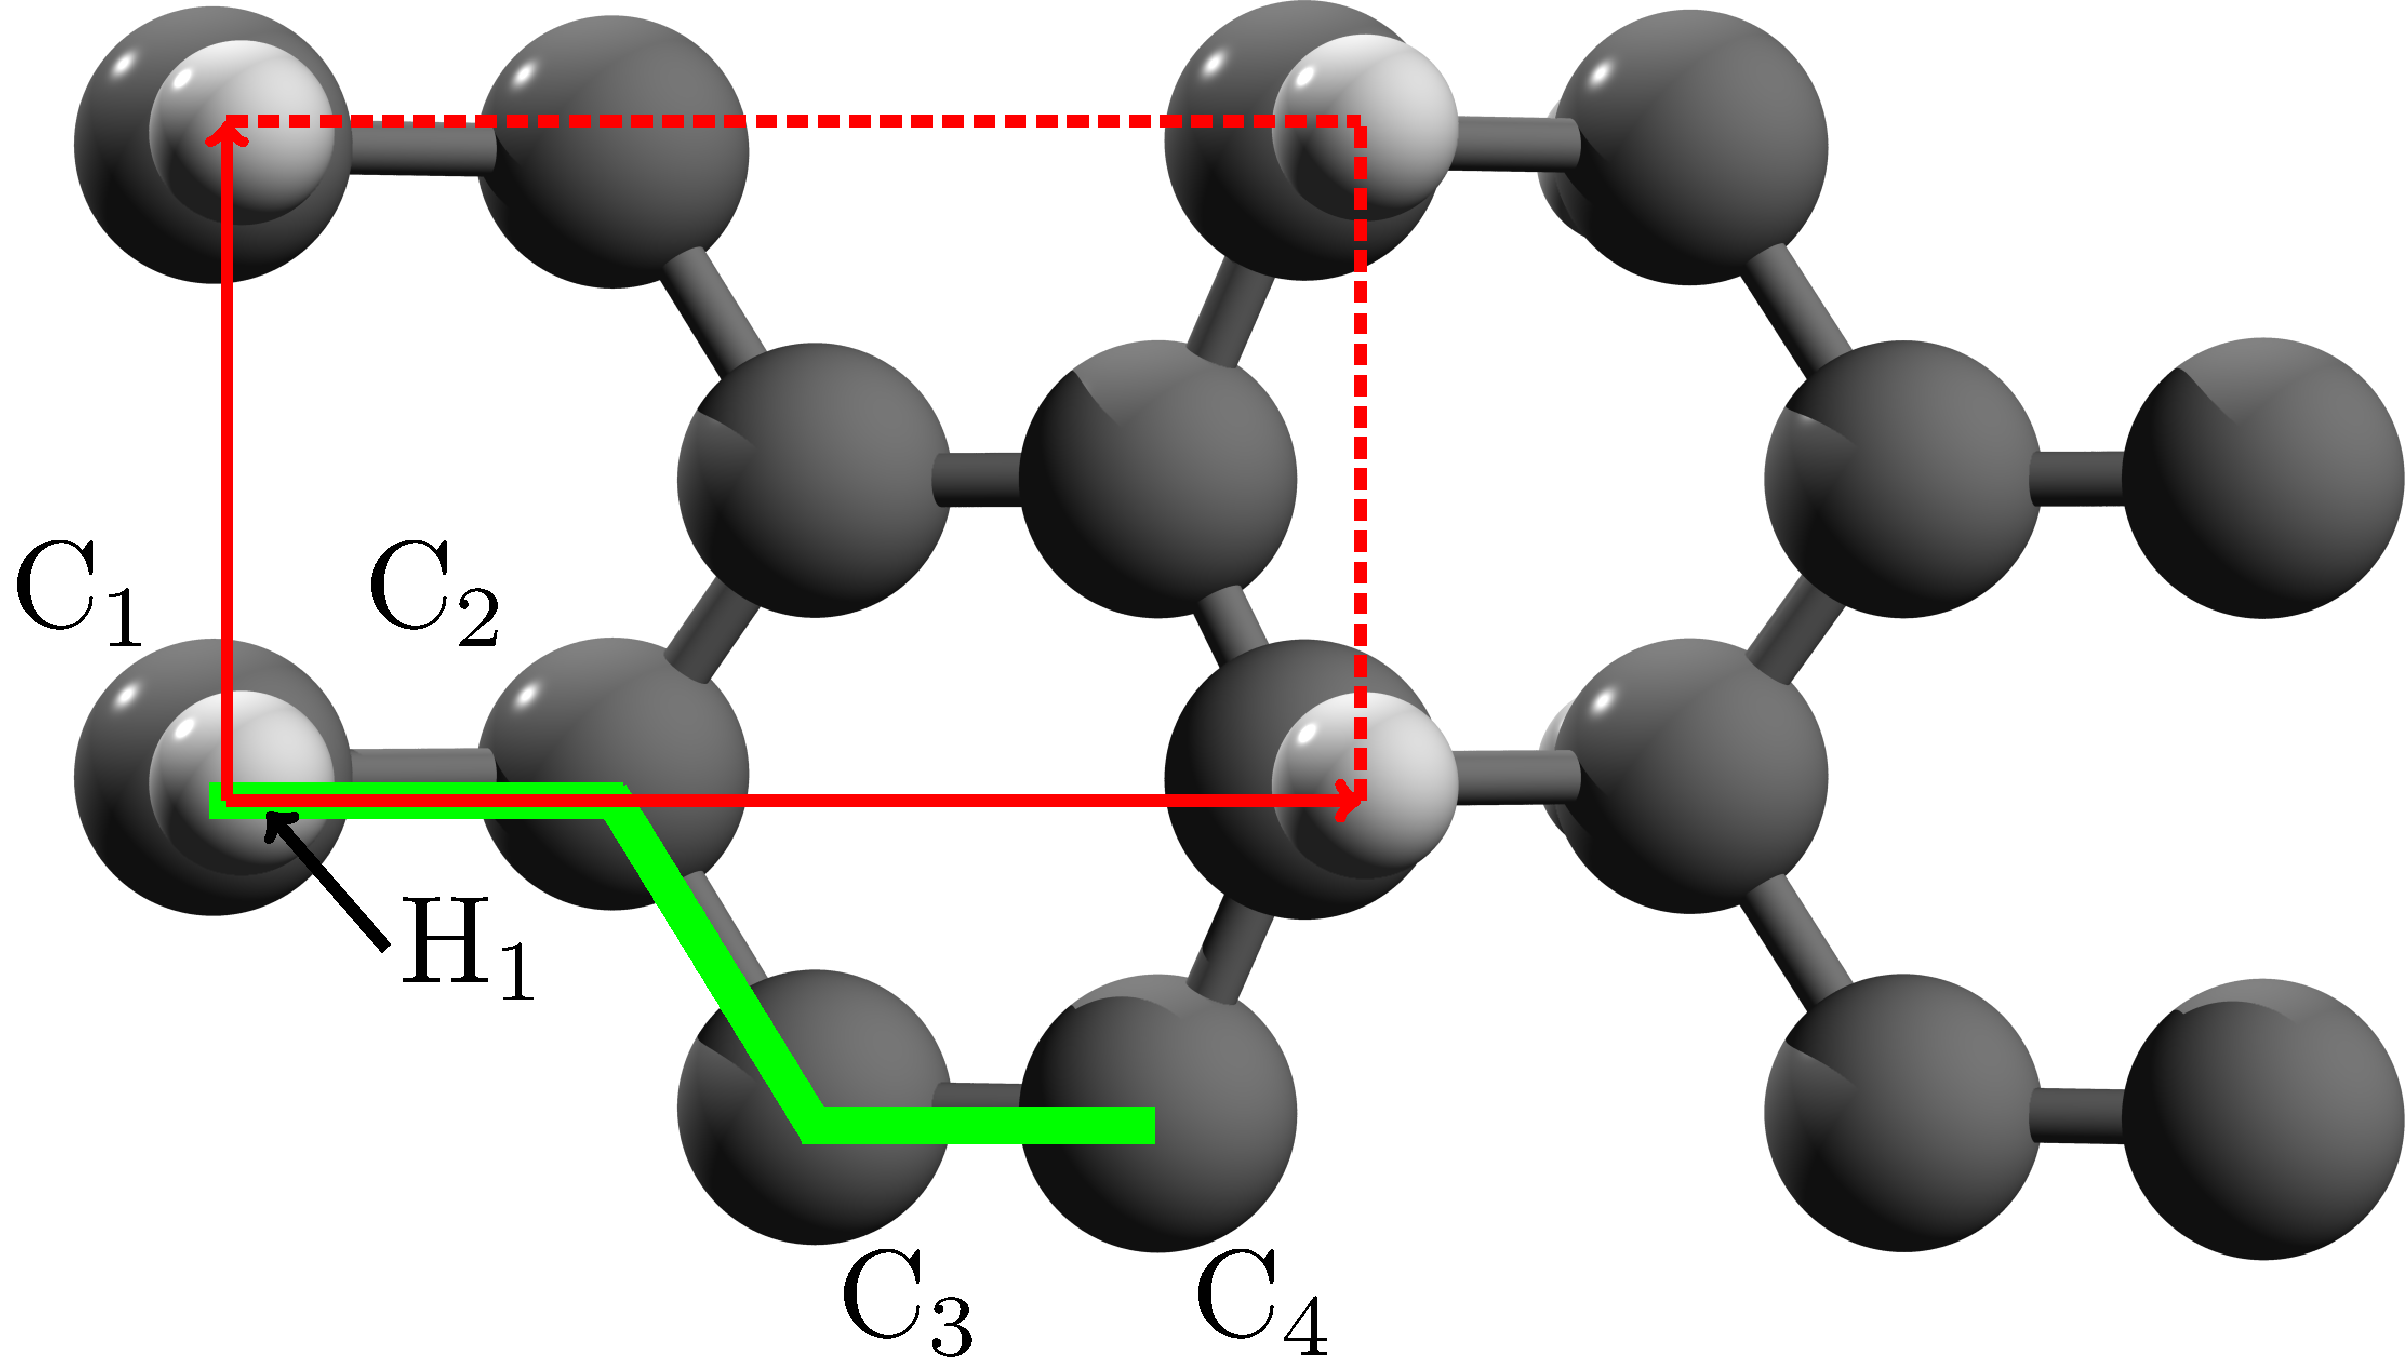
\includegraphics[width=0.9\textwidth]{figs/alt1.pdf}

\vspace{5mm}

\column{0.3\textwidth}
\flushleft
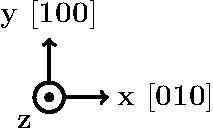
\includegraphics[width=0.9\textwidth]{figs/arrows1.pdf}

\end{columns}

\vspace{-5mm}

\begin{columns}

\column{0.7\textwidth}
\flushright
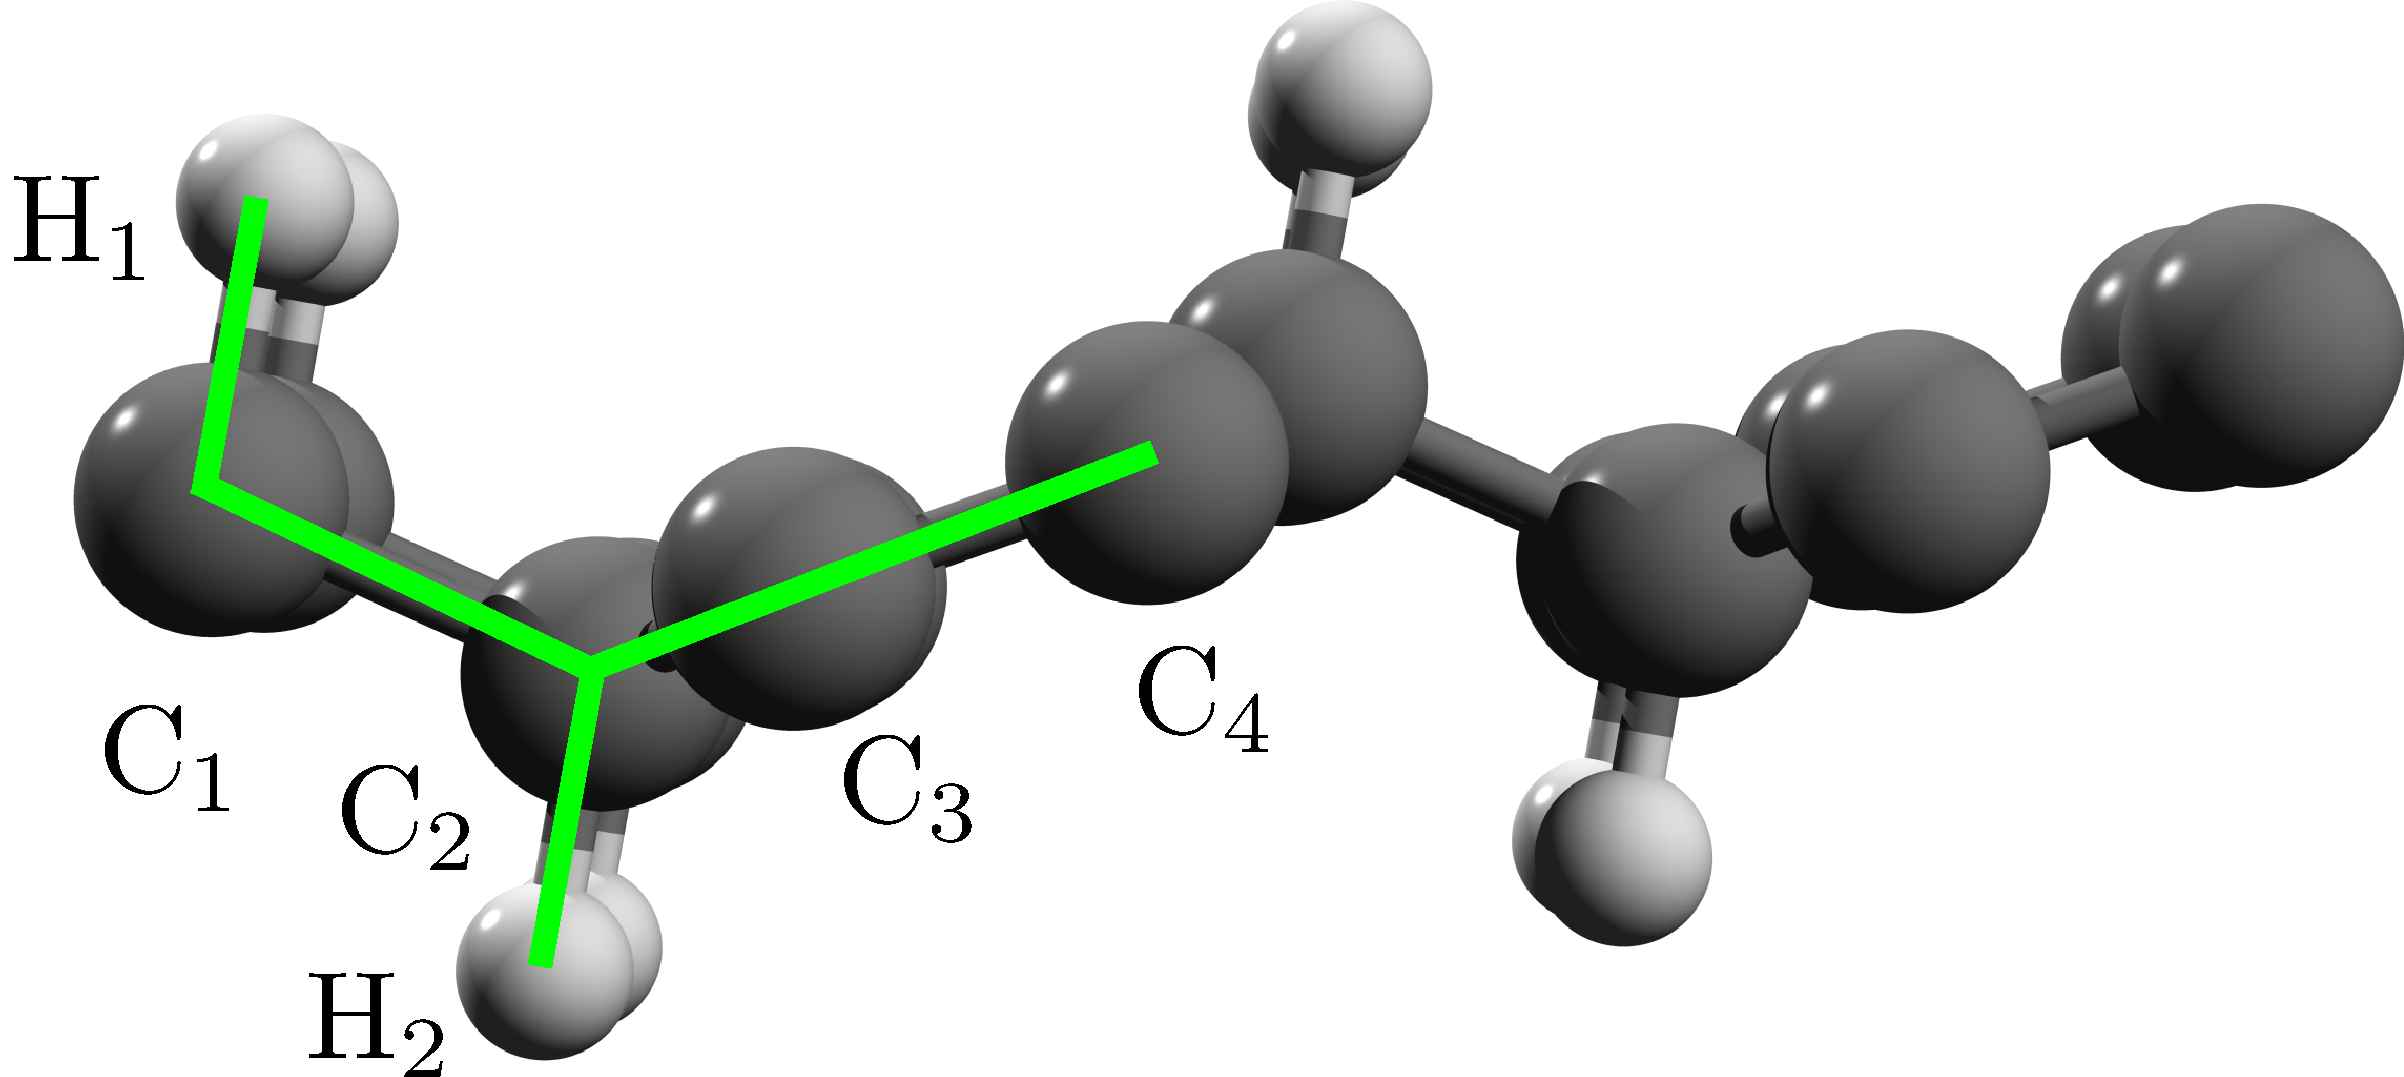
\includegraphics[width=0.9\textwidth]{figs/alt2.pdf}

\vspace{5mm}

\column{0.3\textwidth}
\flushleft
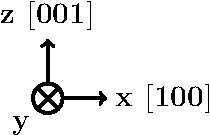
\includegraphics[width=0.9\textwidth]{figs/arrows2.pdf}

\end{columns}

\vspace{-4mm}
\begin{center}
{\Large Alt structure:} 50\% hydrogenation; hydrogen at bot sides.
\end{center}

\end{frame}

%%%%%%%%%%%%%%%%%%%%%%%%%%%%%%%%%%%%%%%%%%%%%%%%%%%%%%%%%%%%%%%%%%%%%%%%%%%%%


%%%%%%%%%%%%%%%%%%%%%%%
\subsection{Up structure}
%%%%%%%%%%%%%%%%%%%%%%%


\begin{frame}

\vspace{-3mm}
\begin{columns}

\column{0.7\textwidth}
\flushright
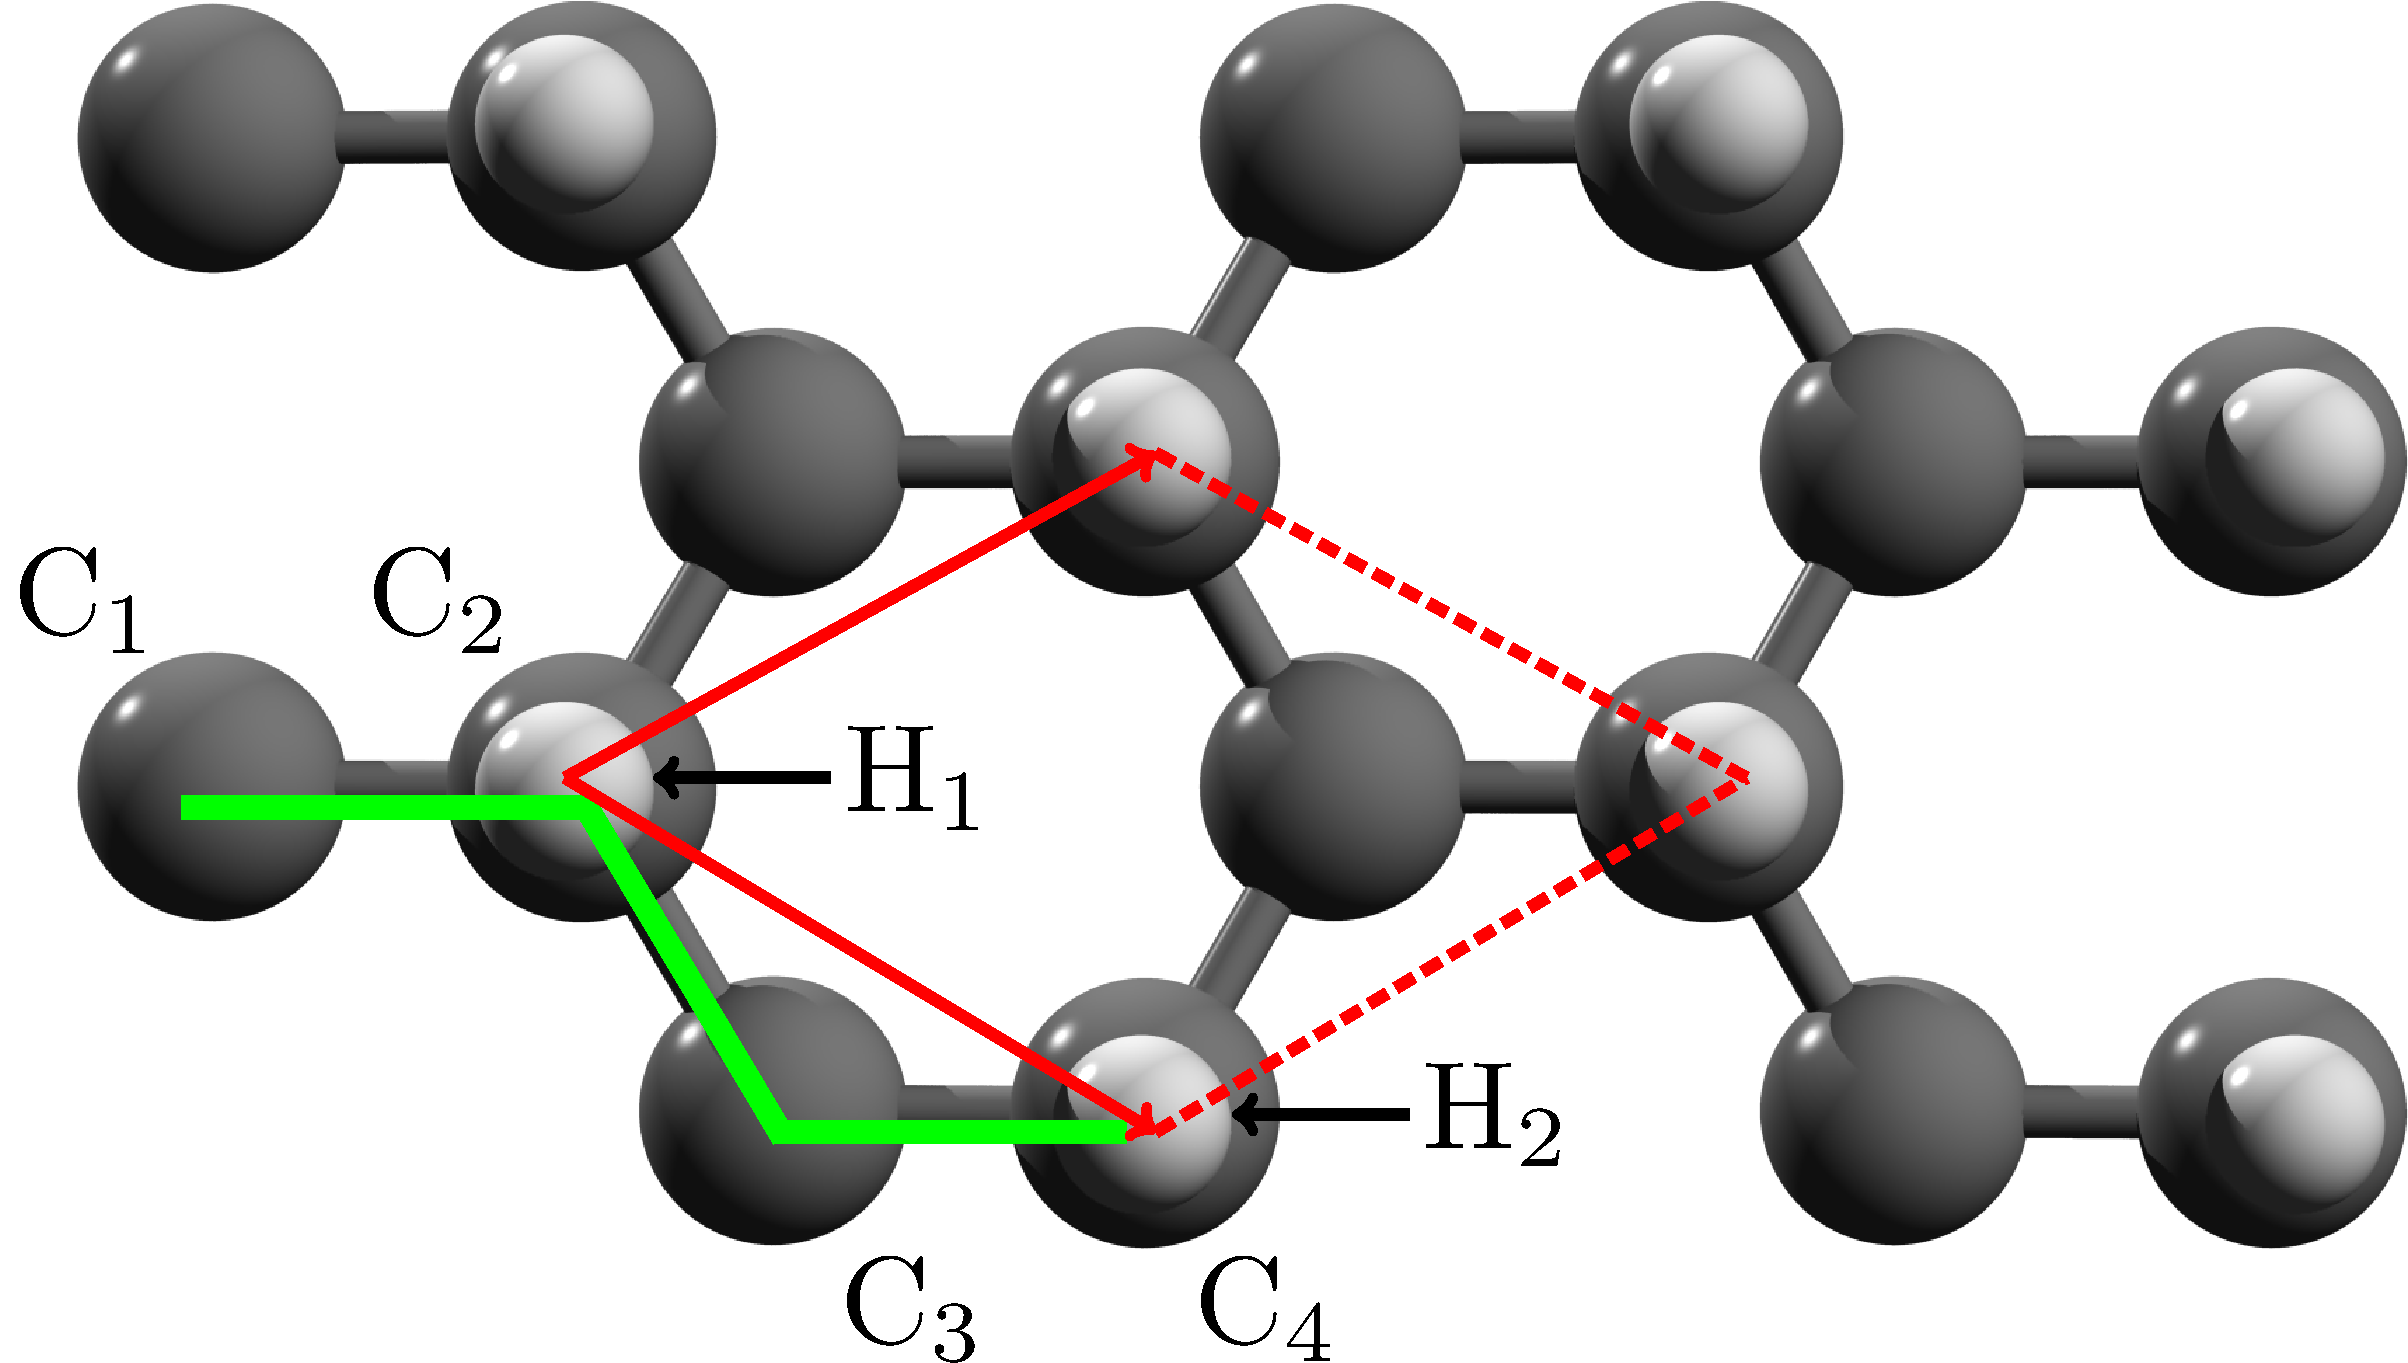
\includegraphics[width=0.9\textwidth]{figs/up1.pdf}

\vspace{5mm}

\column{0.3\textwidth}
\flushleft
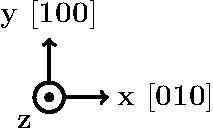
\includegraphics[width=0.9\textwidth]{figs/arrows1.pdf}

\end{columns}

\vspace{-5mm}

\begin{columns}

\column{0.7\textwidth}
\flushright
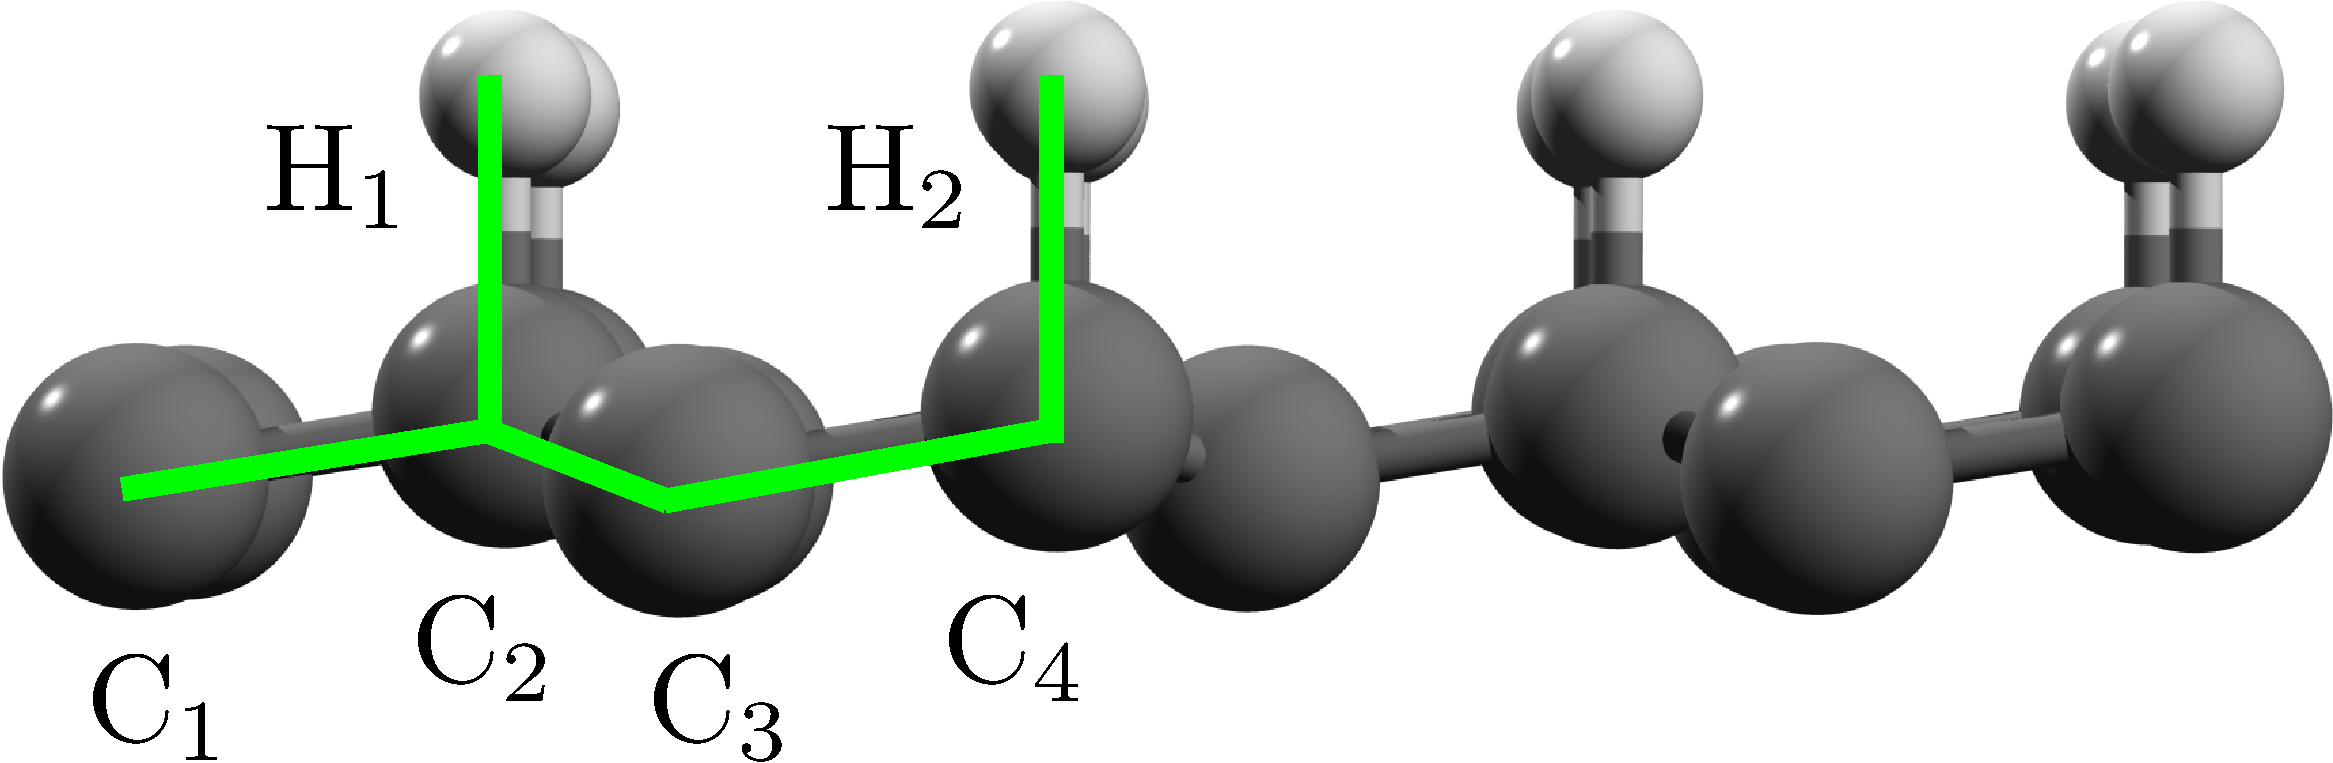
\includegraphics[width=0.9\textwidth]{figs/up2.pdf}

\vspace{5mm}

\column{0.3\textwidth}
\flushleft
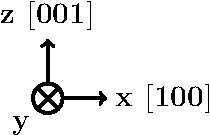
\includegraphics[width=0.9\textwidth]{figs/arrows2.pdf}

\end{columns}

\vspace{-4mm}
\begin{center}
{\Large Up structure:} 50\% hydrogenation; hydrogen on the upper side.
\end{center}

\end{frame}


%%%%%%%%%%%%%%%%%%%%%%%%%%%%%%%%%%%%%%%%%%%%%%%%%%%%%%%%%%%%%%%%%%%%%%%%%%%%%




%%%%%%%%%%%%%%%%%%%%%%%%%%%%%%%%%%%%%%%%%%%%%%%%%%%%%%%%%%%%%%%%%%%%%%%%%%%%%
\section{Theory} 
%%%%%%%%%%%%%%%%%%%%%%%%%%%%%%%%%%%%%%%%%%%%%%%%%%%%%%%%%%%%%%%%%%%%%%%%%%%%%



%%%%%%%%%%%%%%%%%%%%%%%
\subsection{Optical spin injection and DSP}
%%%%%%%%%%%%%%%%%%%%%%%



\begin{frame}

\vspace{-0.2cm}

\noindent\makebox[\linewidth]{\rule{\linewidth}{0.4pt}}

\vspace{-2.0mm}
\begin{center}
{\large Optical spin injection and degree of spin polarization (DSP)}
\end{center}

\vspace{-6mm}
\noindent\makebox[\linewidth]{\rule{\linewidth}{0.4pt}}


{\small

\begin{columns}
    
\column{0.5\textwidth}
\begin{itemize}

\item 
Spintronics is based in the injection, detection and transport of spin
polarized electrons in nonmagnetic materials.\footnote[frame]{\tiny A. Fert et.
al. Rev. Mod. Phys., 80(4):1517, 2008.}

\item 
Spin polarized electrons in a given $a$ direction can be injected through
circularly polarized light.\footnote[frame]{\tiny N. Arzate et al. Phys. Rev.
B, 90(20):205310, 2014.}

\end{itemize}


\column{0.5\textwidth}

\begin{figure}[h!]
\begin{tikzpicture}

\node[anchor=south west,inner sep=0] at (0.2,-0.3) 
{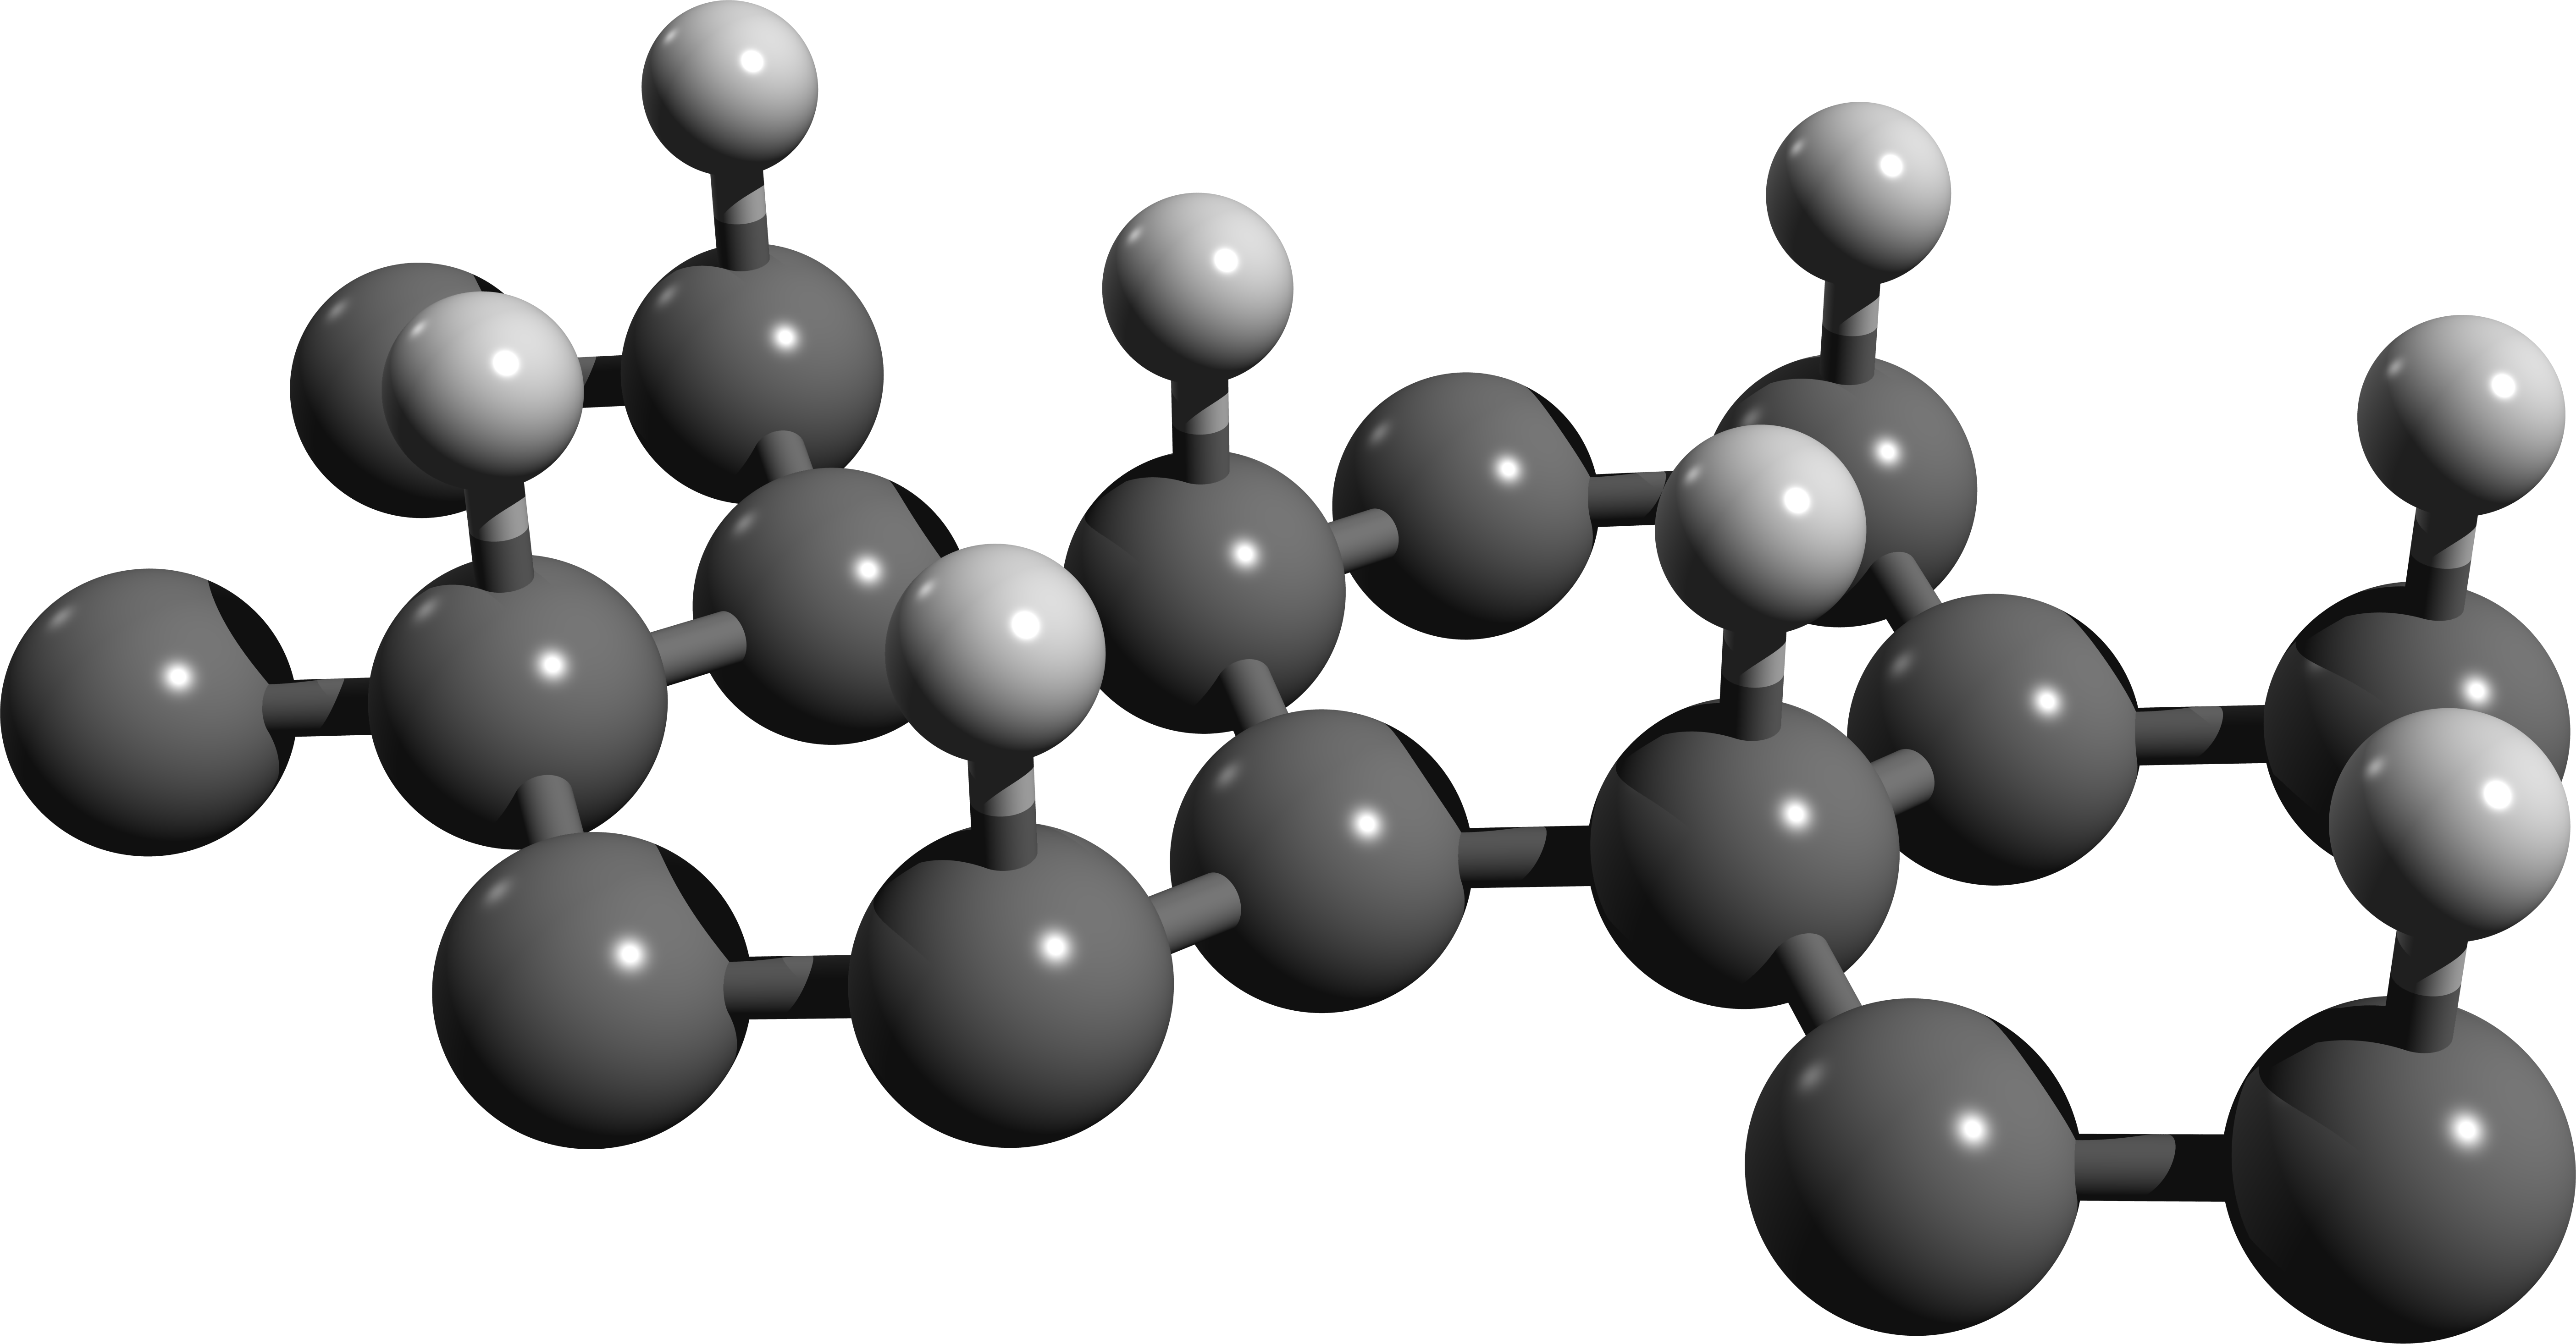
\includegraphics[width=1.0\textwidth]{figs/up3.png}};
\node[anchor=south west,inner sep=0] at (1.5,-1.2) 
{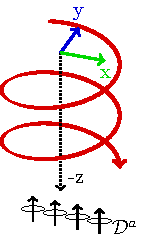
\includegraphics[width=0.6\textwidth]{figs/helix1.pdf}};

\end{tikzpicture}
\end{figure}


\end{columns}

}

\end{frame}

%%%%%%%%%%%%%%%%%%%%%%%%%%%%%%%%%%%%%%%%%%%%%%%%%%%%%%%%%%%%%%%%%%%%%%%%%%%%%

\begin{frame}


{\small

\begin{itemize}

\item 
The Spin generation rate and the carrier generation rate can be written as
\vspace{-4mm}
\begin{align*}
    \dot{S}^{a}(\omega)&= 
\zeta^{abc}(\omega)E^{b}(-\omega)E^{c}(\omega), \\
\dot{n}(\omega)&= 
\xi^{ab}(\omega)E^{a}(-\omega)E^{b}(\omega),
\end{align*}
where $\zeta^{abc}(\omega)$ is the spin injection rate tensor and and $\xi^
{ab}(\omega)$ is the carrier generation rate tensor.

\item 
The degree of spin polarization (DSP) quantifies the fraction of injected
electrons
in the conduction bands that are spin polarized along direction $a$ and is
given by
\vspace{-2mm}
\begin{equation}
\mathcal{D}^{a}(\omega)=
\frac{\dot{S}^{a}(\omega)}{(\hbar/2)\dot{n}(\omega)}
\end{equation}

\item 
DSP is a second order optical effect; it is possible to generate spin
polarized
electrons along three Cartesian directions with an incident circularly polarized
beam.


\end{itemize}
}


\end{frame}


%%%%%%%%%%%%%%%%%%%%%%%%%%%%%%%%%%%%%%%%%%%%%%%%%%%%%%%%%%%%%%%%%%%%%%%%%%%%%


%%%%%%%%%%%%%%%%%%%%%%%
\subsection{Pure spin current injection}
%%%%%%%%%%%%%%%%%%%%%%%


\begin{frame}

\vspace{-0.2cm}

\noindent\makebox[\linewidth]{\rule{\linewidth}{0.4pt}}

\vspace{-2.0mm}
\begin{center}
{\large Pure spin current and spin velocity injection (SVI)}
\end{center}

\vspace{-6mm}
\noindent\makebox[\linewidth]{\rule{\linewidth}{0.4pt}}

\vspace{3mm}
{\Large Pure spin current injection}

\vspace{-4mm}
\begin{columns}

\column{0.40\textwidth}

{\small


\begin{itemize}

\item 
The spin current moves along direction $\mathbf{\hat{a}}$ with the spin
polarized along direction $\mathbf{\hat{b}}$.\footnote[frame]{\tiny A. Najmaie
et. al. Phys. Rev. B, 68(16):165348, 2003.}

\item 
There is no net motion of charge but a spin current is produced.
\textsuperscript{1}

\end{itemize}
}

\column{0.60\textwidth}

\begin{figure}[h!]
\begin{tikzpicture}

\node[anchor=south west,inner sep=0] at (0.2,-0.3) 
{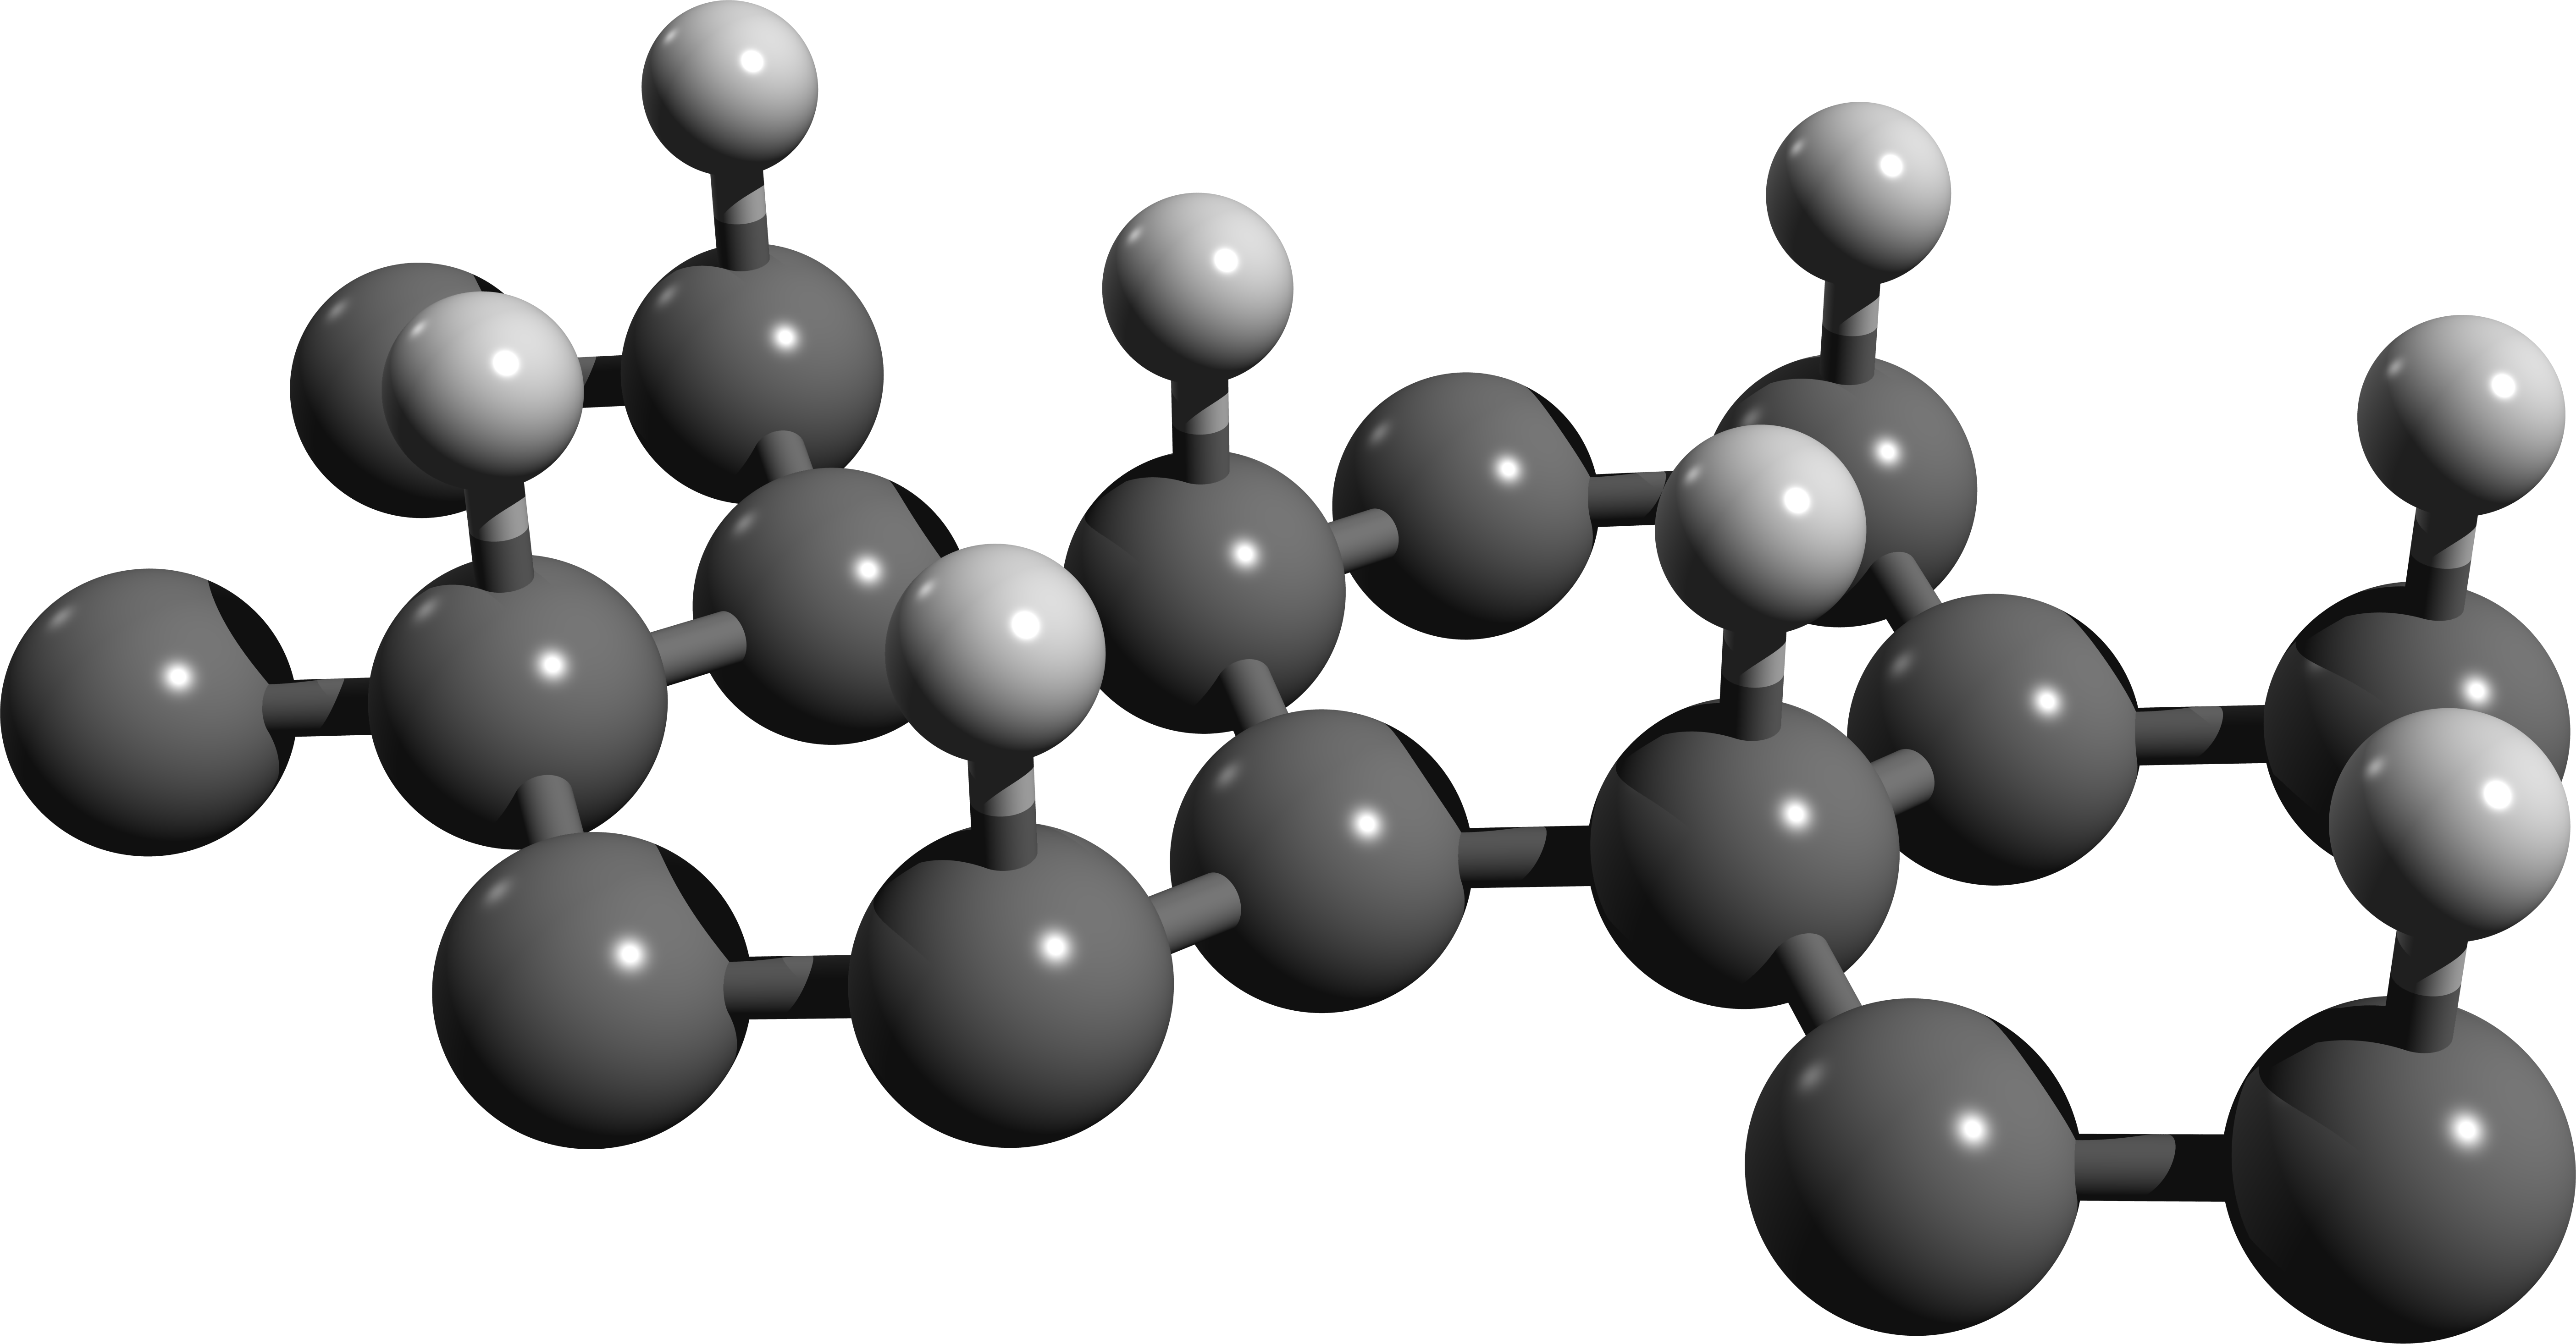
\includegraphics[width=1.0\textwidth]{figs/up3.png}};

\node[anchor=south west,inner sep=0] at (1.5, 1.4) 
{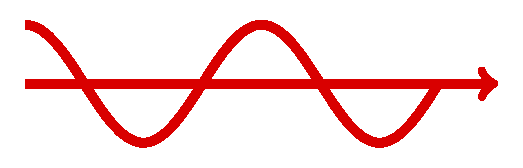
\includegraphics[width=0.55\textwidth,angle=-90,origin=c]
{figs/arrow_1omega.pdf}};

\node[anchor=south west,inner sep=0] at (1.9, 1.3) 
{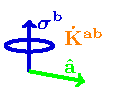
\includegraphics[width=0.40\textwidth]{figs/spin.pdf}};

\end{tikzpicture}
\end{figure}


\end{columns}

\end{frame}

%%%%%%%%%%%%%%%%%%%%%%%%%%%%%%%%%%%%%%%%%%%%%%%%%%%%%%%%%%%%%%%%%%%%%%%%%%%%%

\begin{frame}



\vspace{3mm}

\begin{itemize}

\item 
Is a second-order optical nonlinear effect.

\vspace{3mm}

\item 
A pure spin current can be produced by a single linearly polarized beam in
noncentrosymmetric materials\footnote[frame]{\tiny A. Najmaie
et. al. Phys. Rev. B, 68(16):165348, 2003.} and is given by\footnote[frame]
{\tiny Reinaldo Zapata-Pe\~na et. al. Phys. Rev. B 96, 195415. 2017}
% \vspace{-2mm}
\begin{equation}
\dot{K}^{\mathrm{ab}}(\omega) =
\mu^{\mathrm{abcd}}(\omega)
E^{\mathrm{c}}(\omega) E^{\mathrm{d*}}(\omega),
\label{eq:dotk}
\end{equation}
where $\mu^{\mathrm{abcd}}(\omega)$ is the pseudotensor that describes the rate
of change of the PSC.

\end{itemize}

\end{frame}

%%%%%%%%%%%%%%%%%%%%%%%%%%%%%%%%%%%%%%%%%%%%%%%%%%%%%%%%%%%%%%%%%%%%%%%%%%%%%

\begin{frame}

{\Large Spin velocity injection}

\vspace{6mm}

\begin{columns}

\column{0.6\textwidth}

\vspace{-8mm}
\begin{figure}[h!]
\begin{tikzpicture}

\node[anchor=south west,inner sep=0,opacity=0.40] at (0.2,-0.3) 
{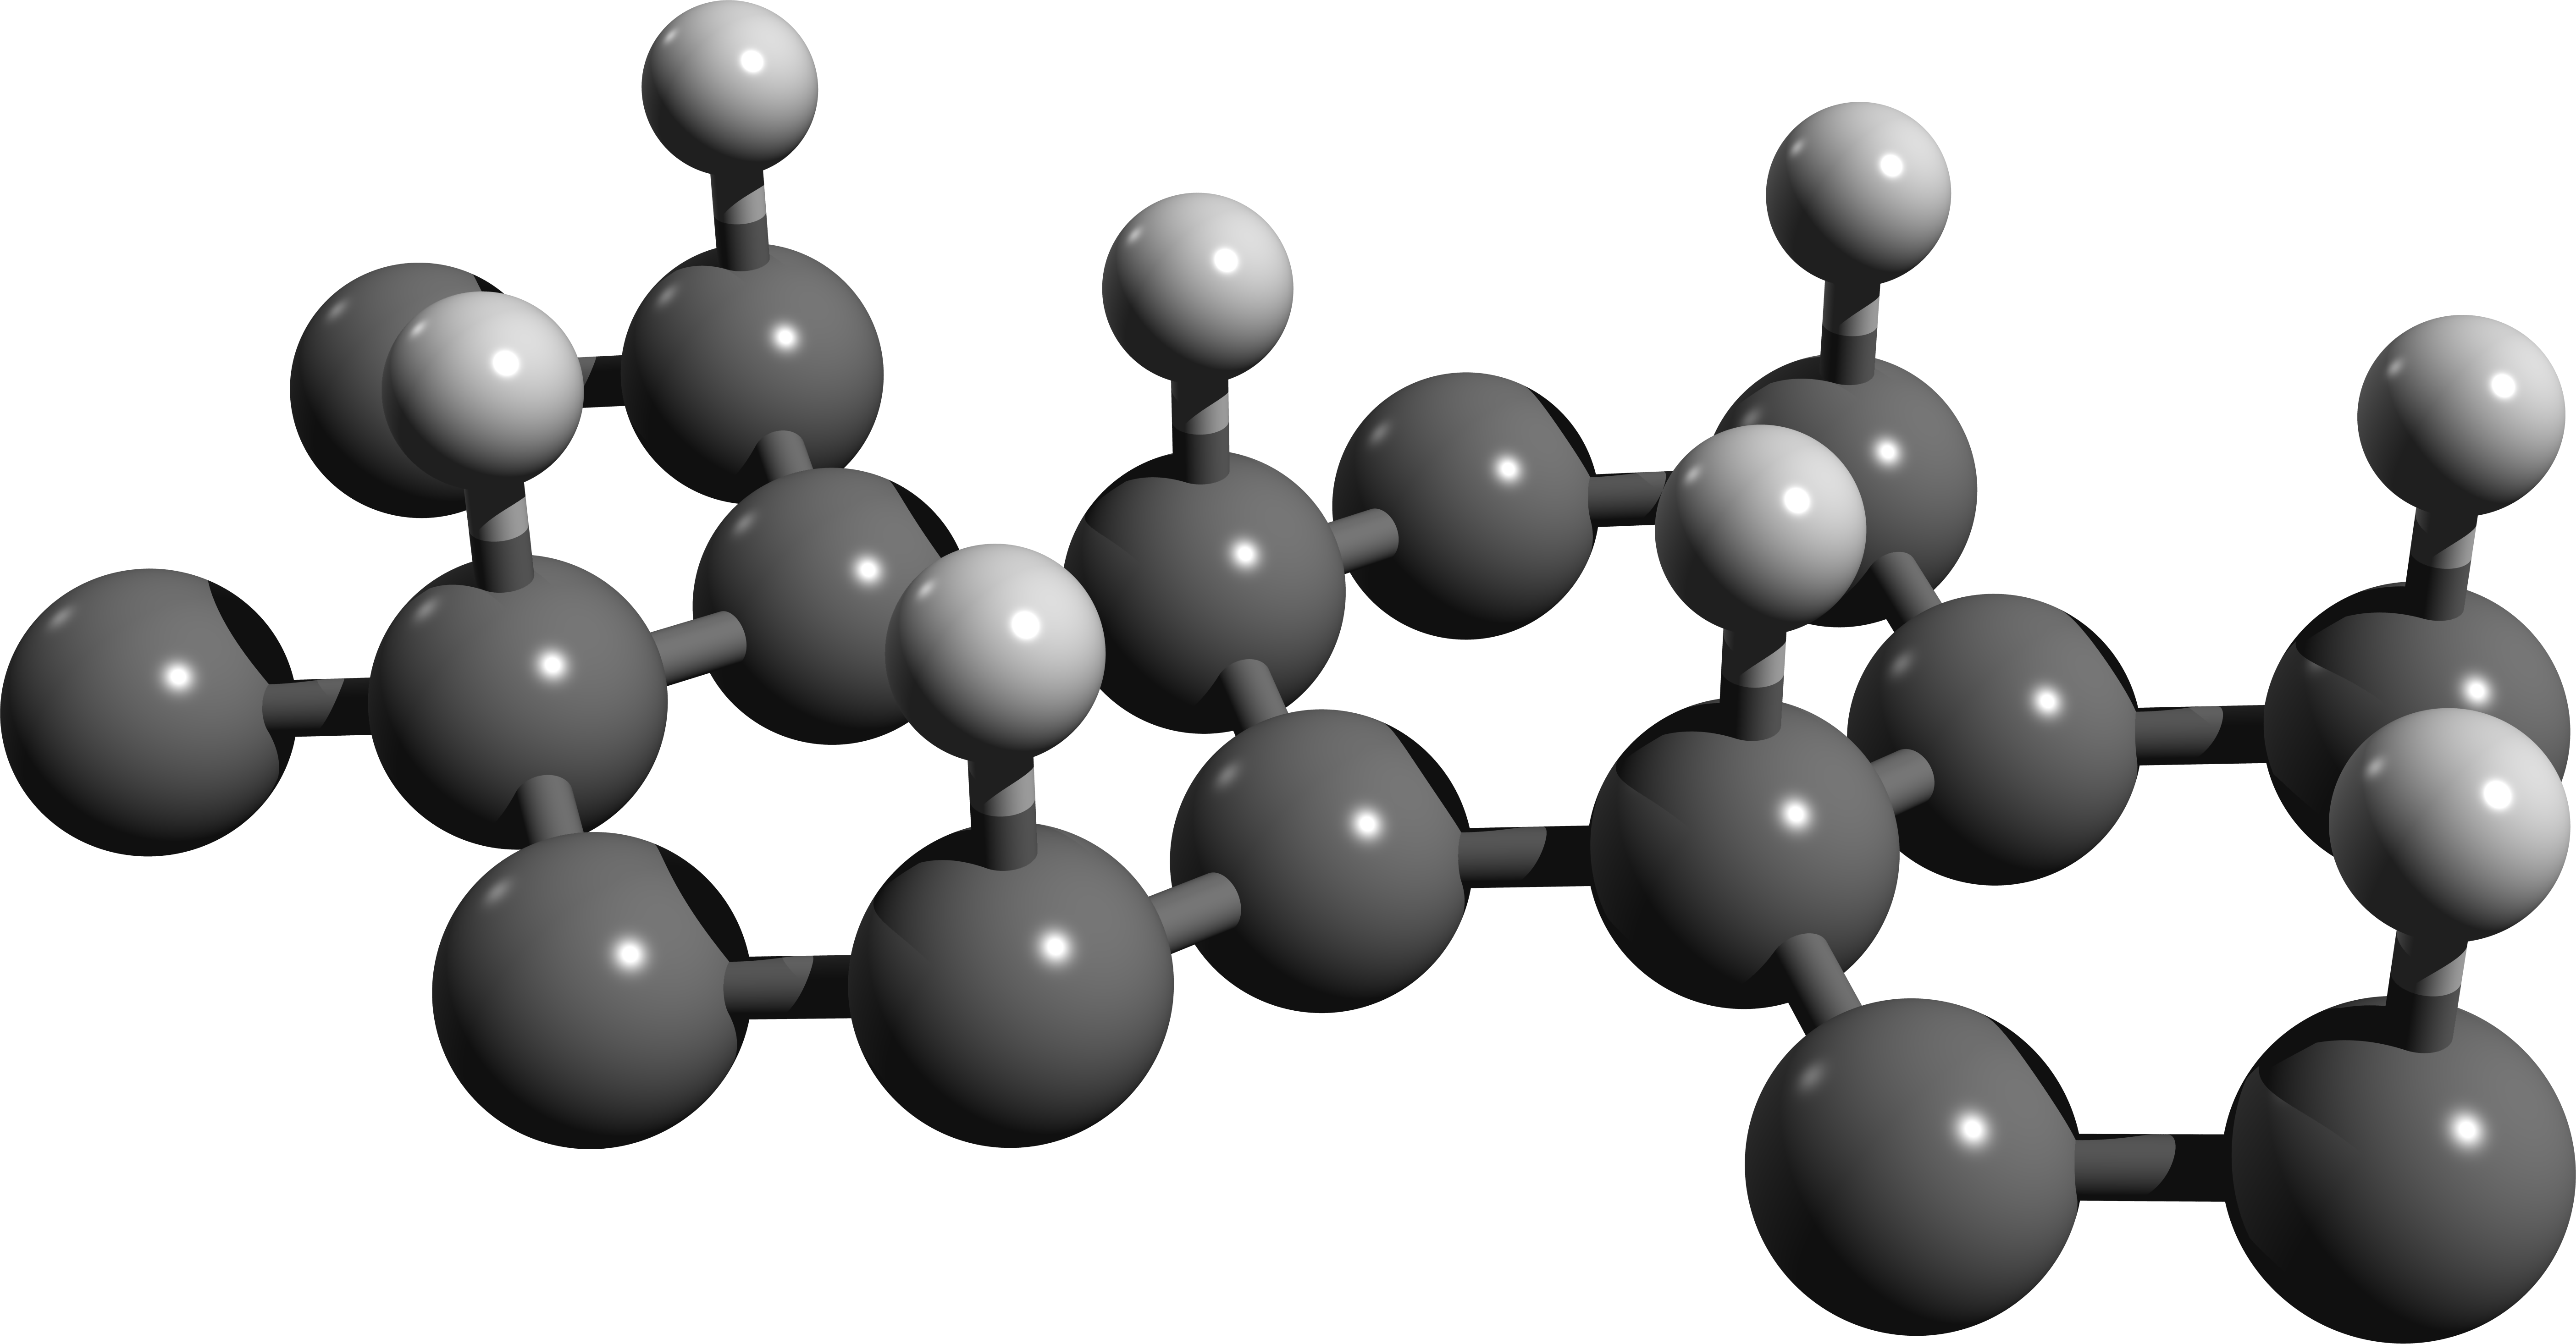
\includegraphics[width=1.0\textwidth]{figs/up3.png}};

\node[anchor=south west,inner sep=0] at (1.5, 1.4) 
{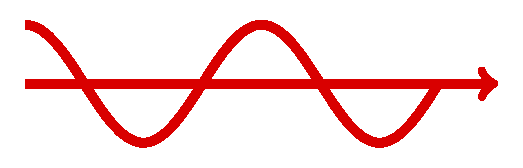
\includegraphics[width=0.55\textwidth,angle=-90,origin=c]
{figs/arrow_1omega.pdf}};

\node[anchor=south west,inner sep=0] at (2.00, 0.3) 
{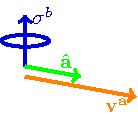
\includegraphics[width=0.6\textwidth]{figs/spinvel.pdf}};

\end{tikzpicture}
\end{figure}

\column{0.45\textwidth}

\begin{itemize}
\item 
The spin velocity injection is defined as\footnote[frame]
{\tiny Reinaldo Zapata-Pe\~na et. al. Phys. Rev. B 96, 195415. 2017}
\begin{equation}\label{eq:vab-w}
\mathcal{V}^{\mathrm{ab}}(\omega) \equiv
\frac{\dot{K}^{\mathrm{ab}}(\omega)}{(\hbar/2) \dot{n}(\omega)},
\end{equation}
which gives the velocity, along direction $\hat{\mathbf{a}}$, at which the spin
moves in a polarized state along direction $\hat{\mathbf{b}}$.
\end{itemize}

\end{columns}


\end{frame}

%%%%%%%%%%%%%%%%%%%%%%%%%%%%%%%%%%%%%%%%%%%%%%%%%%%%%%%%%%%%%%%%%%%%%%%%%%%%%

\begin{frame}

{\small

\begin{columns}

\column{0.5\textwidth}

\begin{itemize}

\item 
With 2D structures we can use the  direction of the polarized  electric field
to control ${\cal V}^{\mathrm{a}\mathrm{b}}(\omega)$.

\vspace{3mm}

\item 
Writing ${\mathbf E}(\omega) =
E_0(\omega)(\cos\alpha\,\hat{\mathbf x}+\sin\alpha\,\hat{\mathbf y})$, where
$\alpha$ is the polarization angle, we obtain that
\begin{align}
\mathcal{V}&^{\mathrm{ab}}(\omega,\alpha)
= 
\frac{2}{\hbar\xi(\omega)}
\left(\mu^{\mathrm{abxx}}(\omega)\cos^{2}\alpha + \right. \nonumber \\
&\left. \mu^{\mathrm{abyy}}(\omega)\sin^{2}\alpha + 
\mu^{\mathrm{abxy}}(\omega)\sin 2\alpha\right).
\label{eq:vab-aw}
\end{align}

\end{itemize}

\column{0.5\textwidth}

\vspace{-4mm}

\begin{figure}[h!]
\begin{tikzpicture}

\node[anchor=south west,inner sep=0] at (0.2,-1.0) 
{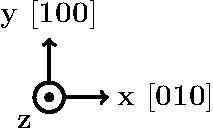
\includegraphics[width=0.4\textwidth]{figs/arrows1.pdf}};

\node[anchor=south west,inner sep=0,opacity=0.5] at (0.2,-0.3) 
{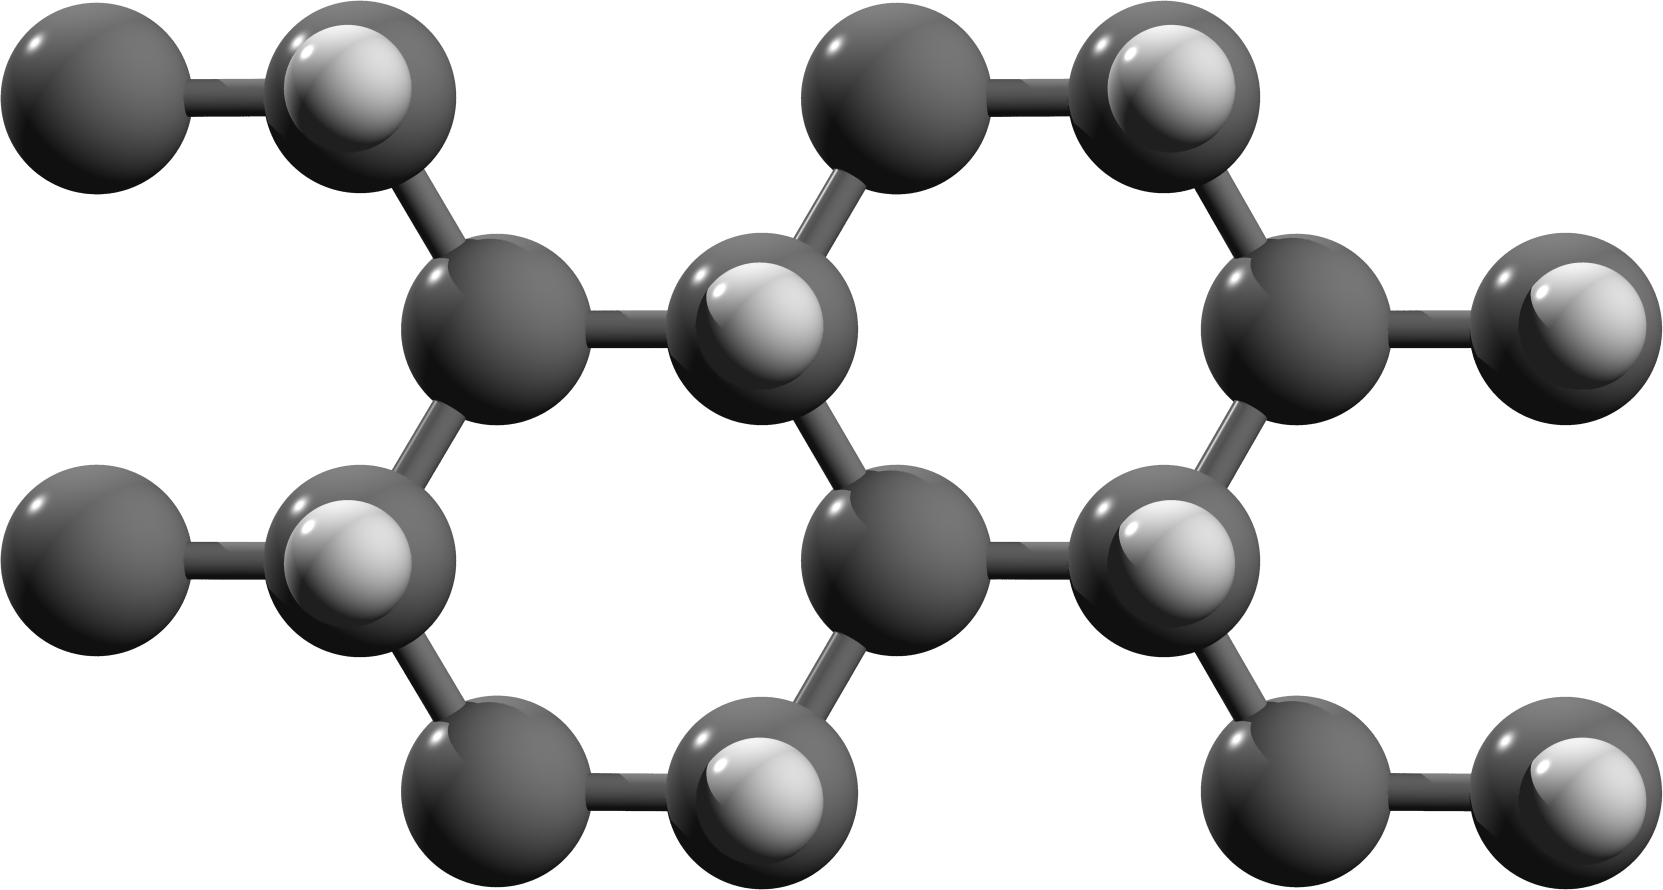
\includegraphics[width=1.0\textwidth]{figs/up1.png}};

\node[anchor=south west,inner sep=0] at (1.8,0.3) 
{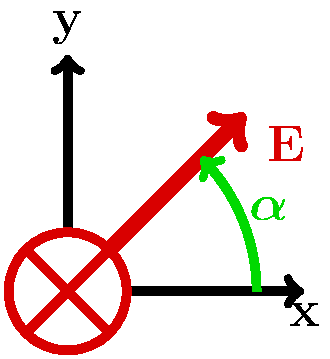
\includegraphics[width=0.40\textwidth]{figs/perp.pdf}};

\end{tikzpicture}
\end{figure}

\vspace{-14mm}

\begin{figure}[h!]
\begin{tikzpicture}


\node[anchor=south west,inner sep=0,opacity=0.5] at (0.2,-0.3) 
{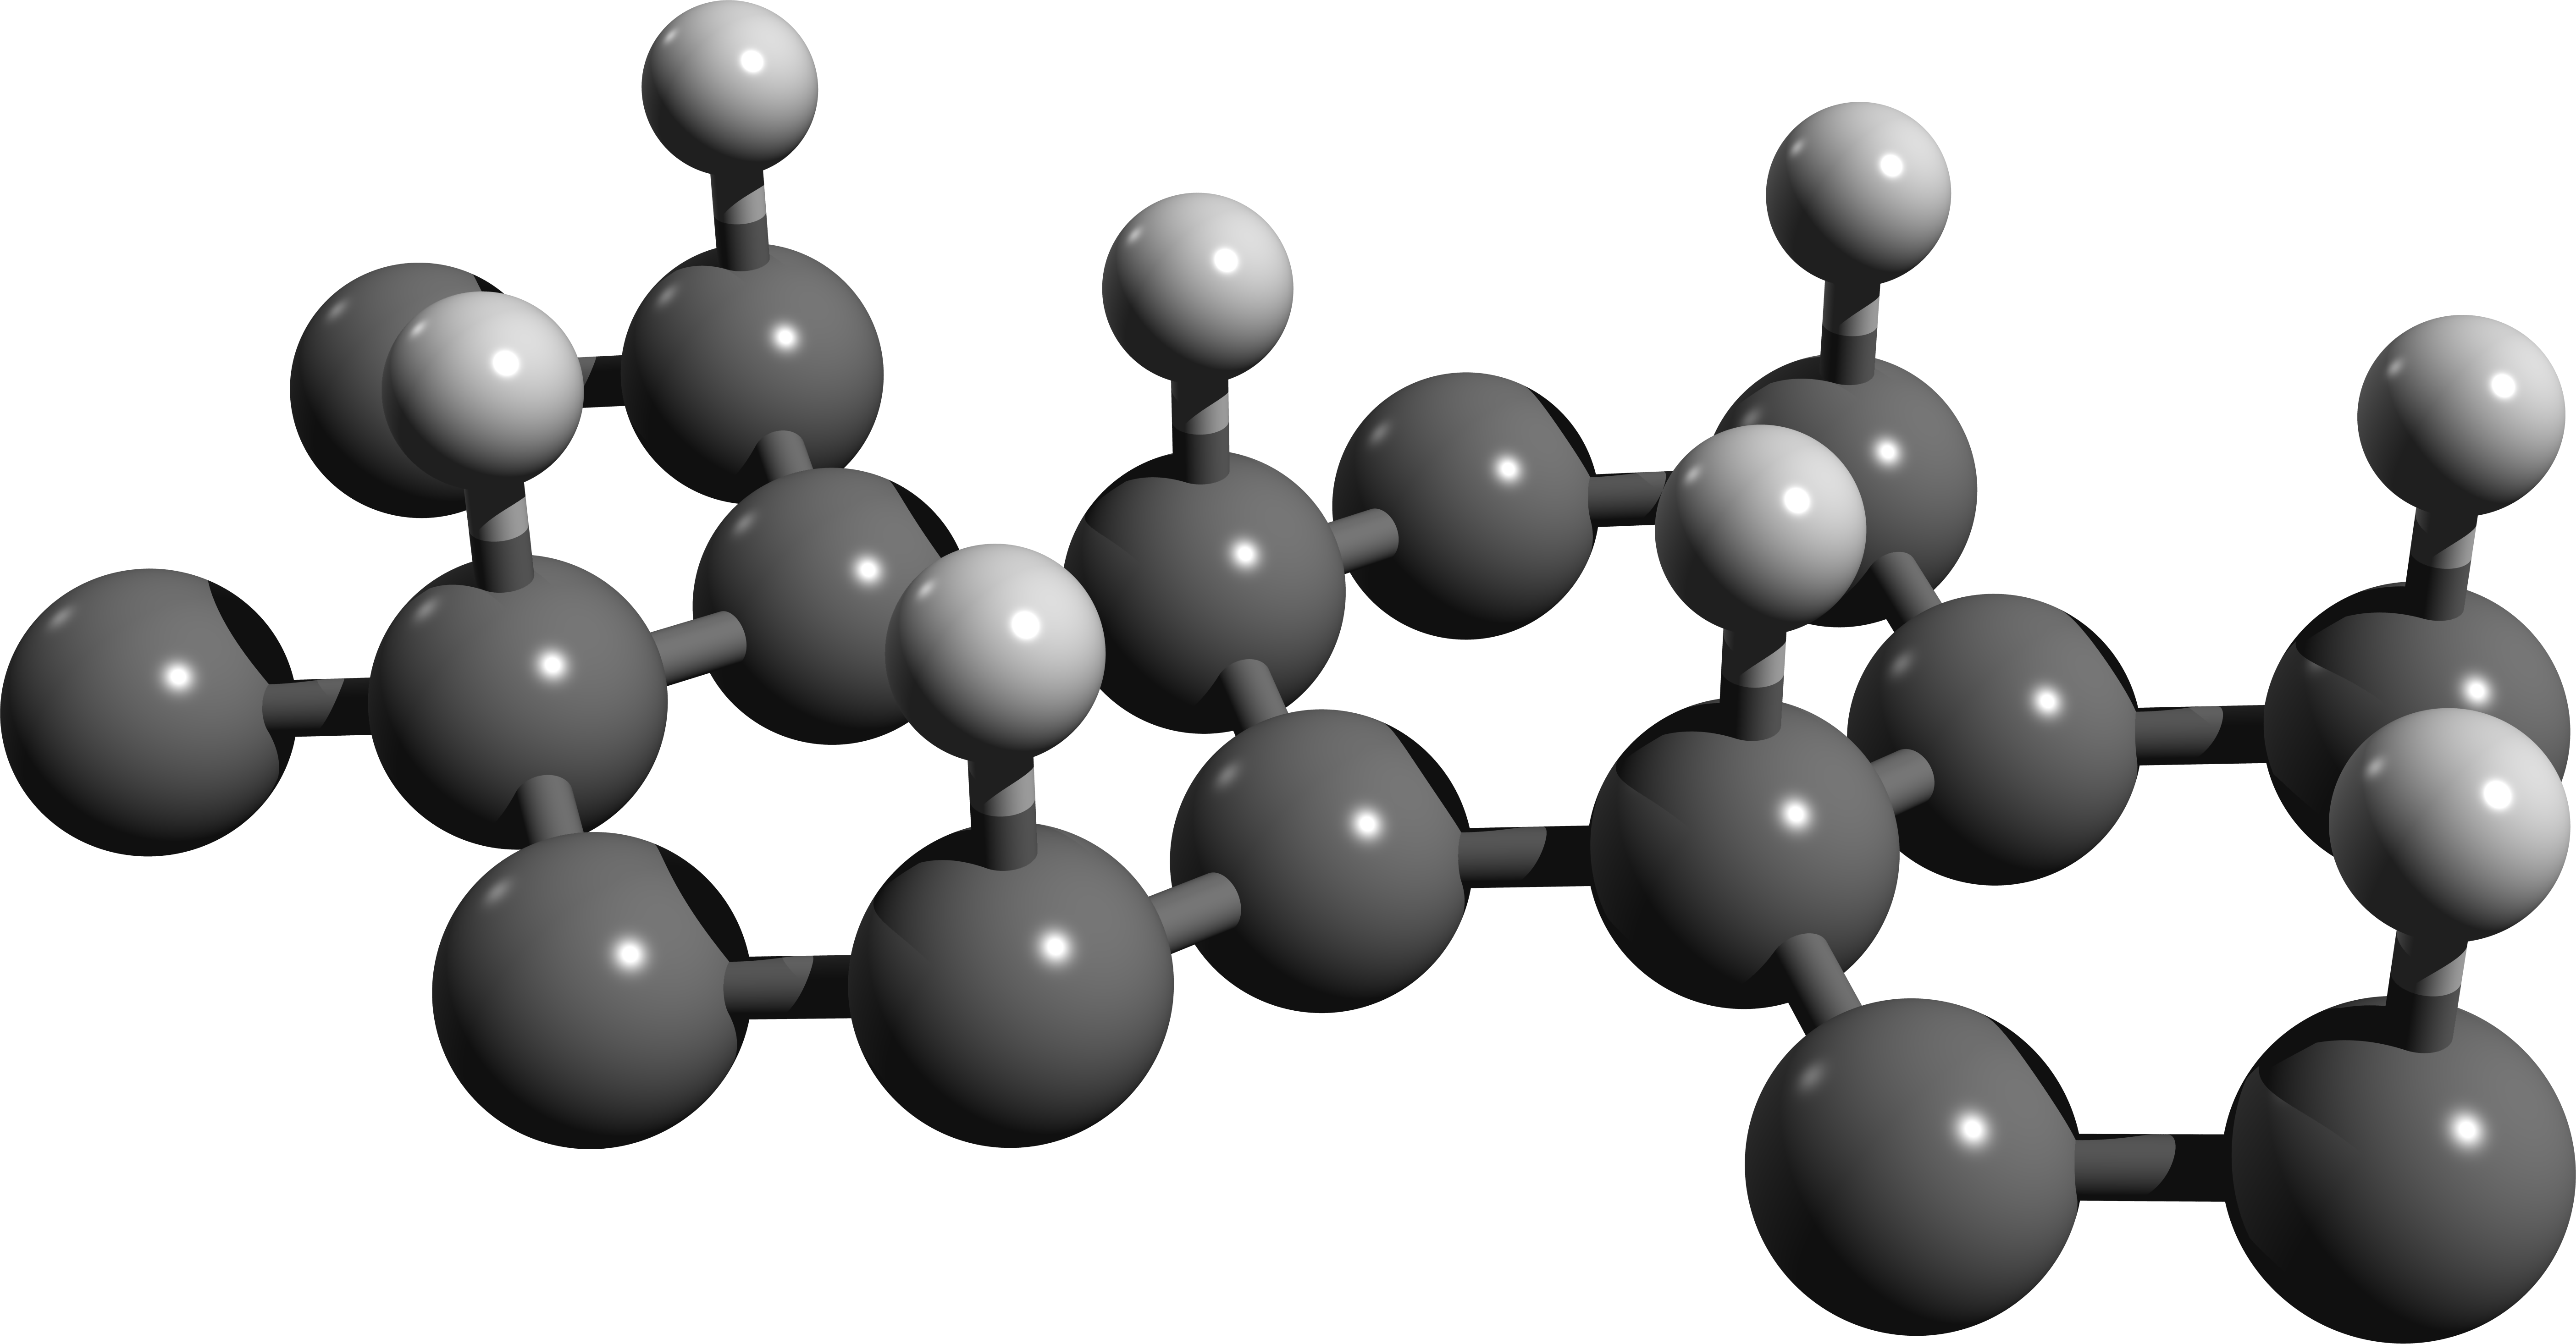
\includegraphics[width=1.0\textwidth]{figs/up3.png}};

\node[anchor=south west,inner sep=0] at (0.0,-0.7) 
{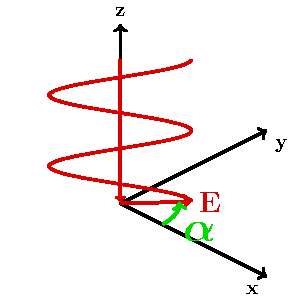
\includegraphics[width=0.8\textwidth]{figs/coord.pdf}};

\end{tikzpicture}
\end{figure}


\end{columns}

}

\end{frame}


%%%%%%%%%%%%%%%%%%%%%%%%%%%%%%%%%%%%%%%%%%%%%%%%%%%%%%%%%%%%%%%%%%%%%%%%%%%%%

%%%%%%%%%%%%%%%%%%%%%%%
\subsection{Fixing the spin polarization}
%%%%%%%%%%%%%%%%%%%%%%%

\begin{frame}

{\Large Fixing the spin polarization\footnote[frame]
{\tiny Reinaldo Zapata-Pe\~na et. al. Phys. Rev. B 96, 195415. 2017}}

{\small

\begin{columns}

\column{0.55\textwidth}

\begin{center}
{\large Spin fixed along $z$ direction}
\end{center}

\vspace{-5mm}

\begin{figure}[h!]
\begin{tikzpicture}


\node[anchor=south west,inner sep=0,opacity=0.40] at (0.2,-0.3) 
{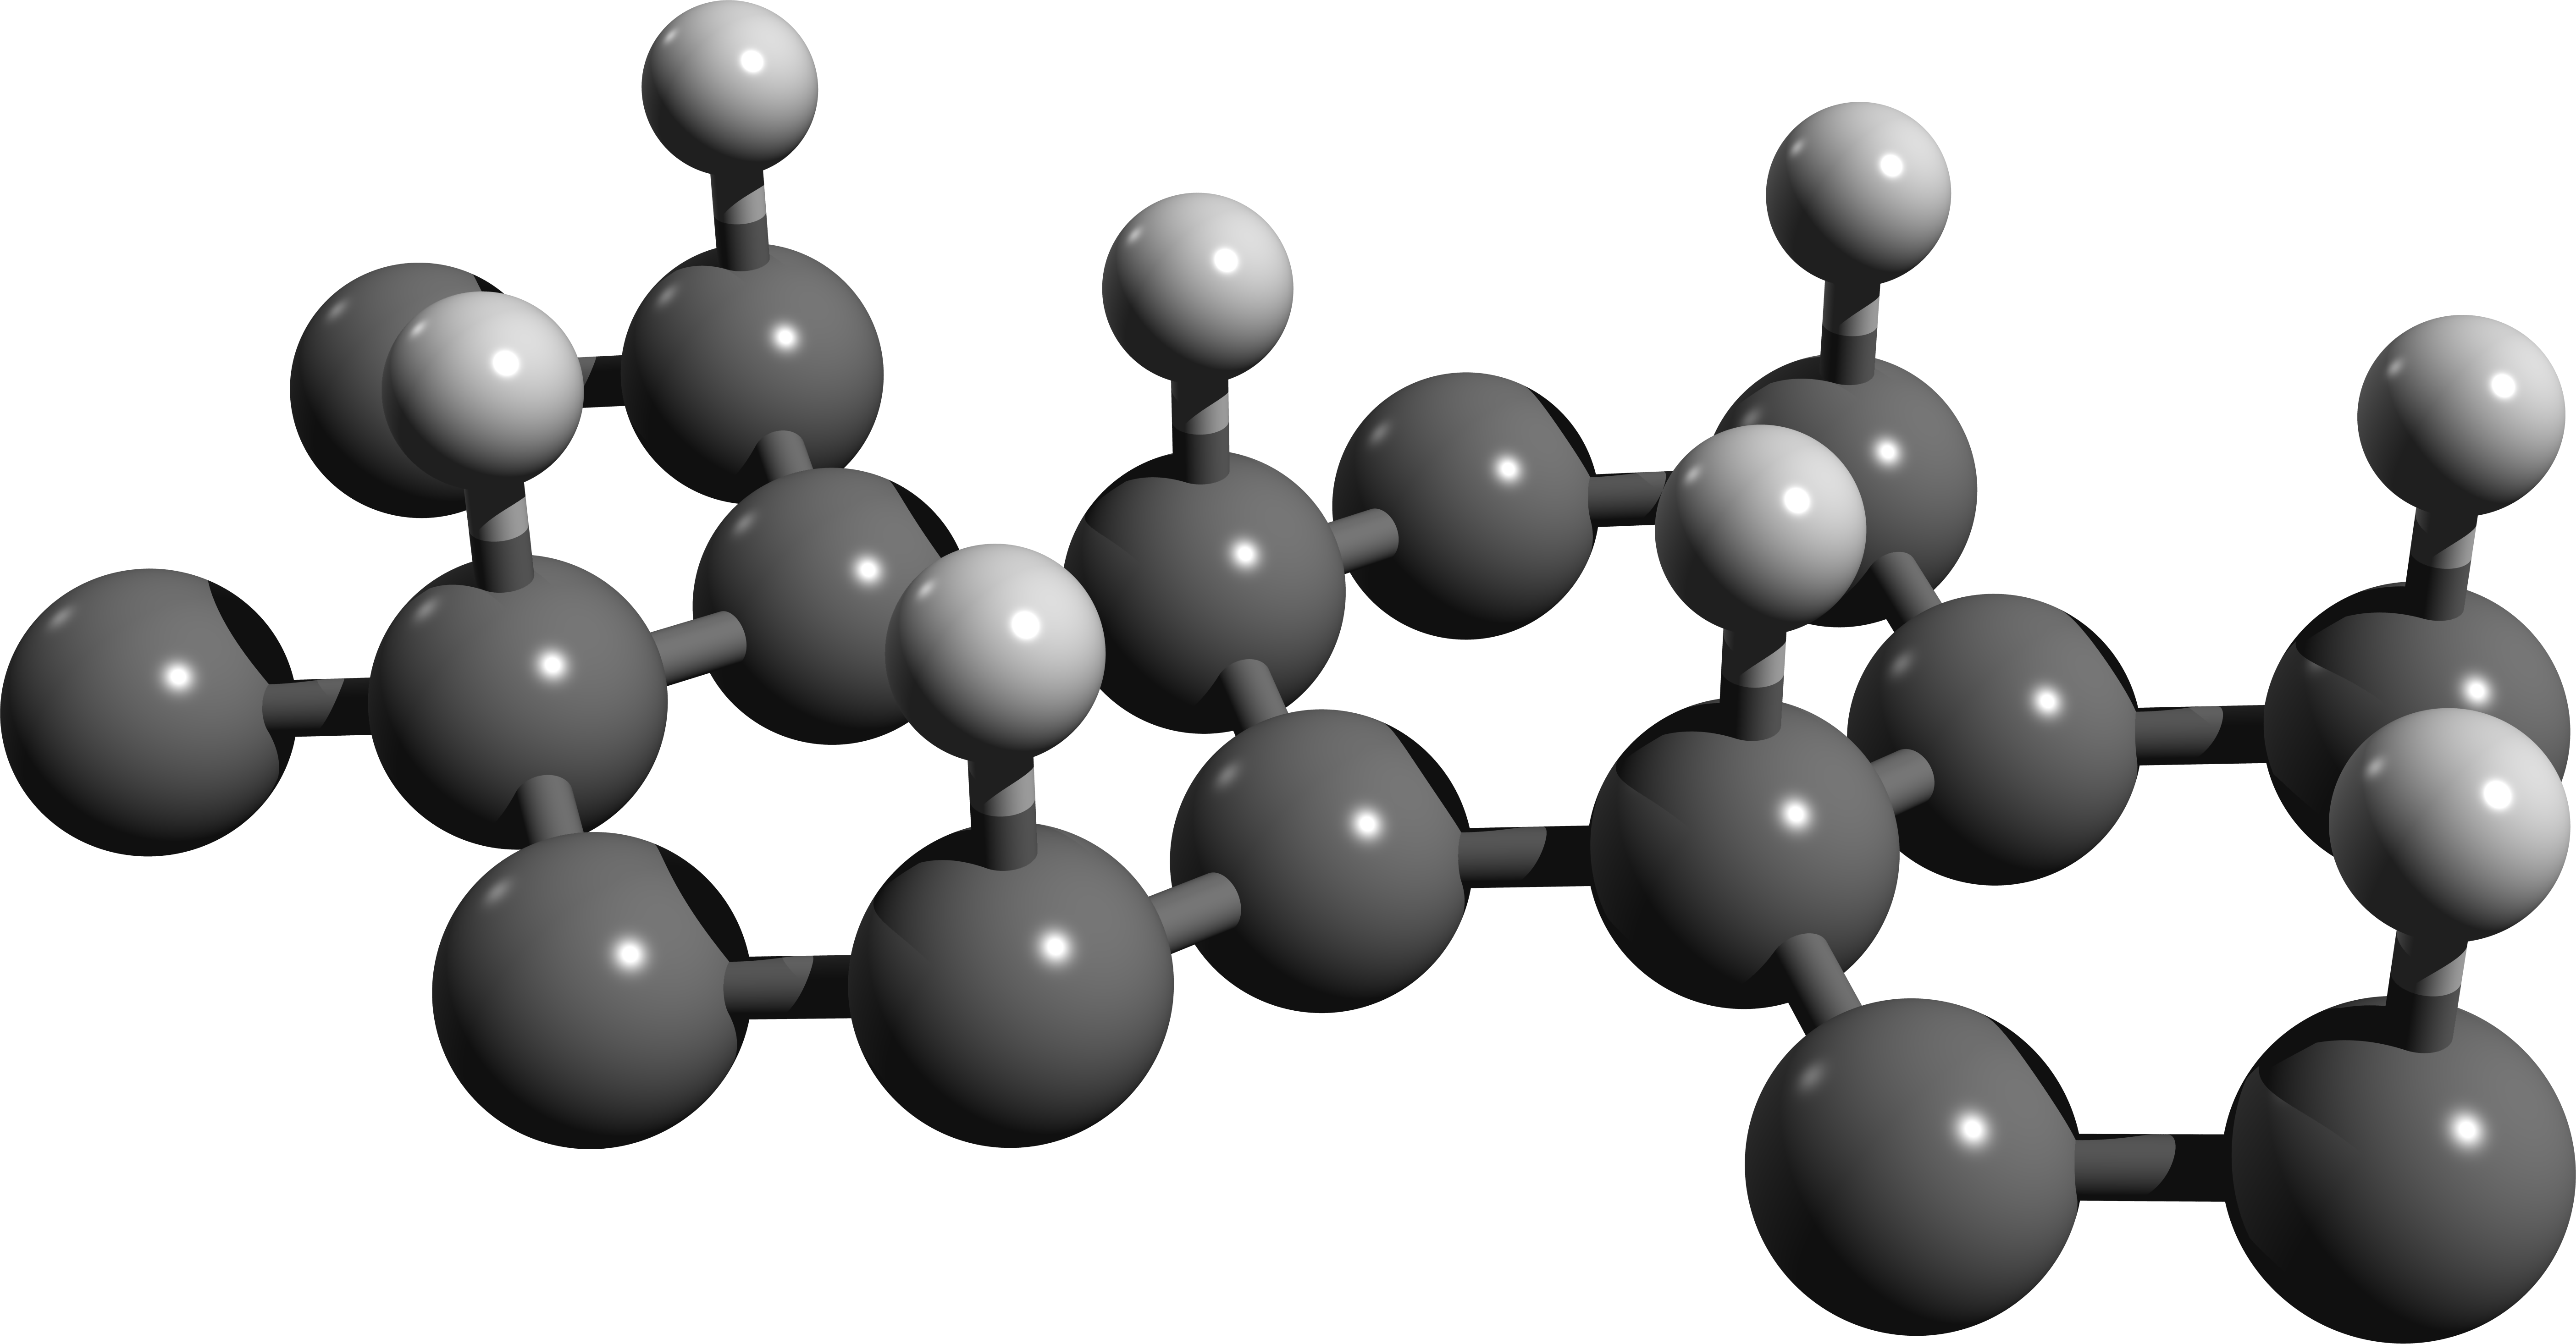
\includegraphics[width=1.0\textwidth]{figs/up3.png}};

\node[anchor=south west,inner sep=0] at (0.6,-0.4) 
{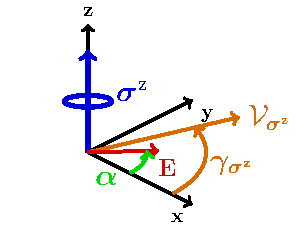
\includegraphics[width=0.85\textwidth]{figs/coord2.pdf}};

\end{tikzpicture}
\end{figure}

\column{0.5\textwidth}

\begin{itemize}

\item Magnitude of the velocity when the spin is fixed in the $\mathbf{b}$
direction 
\begin{align}
\hspace{-4mm}
\mathcal{V}_{\sigma^{\mathrm{b}}}&(\omega,\alpha)
\equiv \nonumber \\ 
&\sqrt{
\left(\mathcal{V}^{\mathrm{xb}}(\omega,\alpha)\right)^{2}\ +
\left(\mathcal{V}^{\mathrm{yb}}(\omega,\alpha)\right)^{2}\ }
\label{eq:vs-mag}
\end{align}

\item 
Angle of the velocity when the spin is fixed in the $\mathbf{b}$
\begin{equation}
\gamma_{\sigma^\mathrm{b}} (\omega,\alpha)
=
\tan^{-1} \left( \frac{\mathcal{V}^{\mathrm{yb}}(\omega,\alpha)}
{\mathcal{V}^{\mathrm{xb}}(\omega,\alpha)} \right)
\label{eq:gamma-ang}
\end{equation}

\end{itemize}
    

\end{columns}

}

\end{frame}

%%%%%%%%%%%%%%%%%%%%%%%%%%%%%%%%%%%%%%%%%%%%%%%%%%%%%%%%%%%%%%%%%%%%%%%%%%%%%

\begin{frame}

{\small

\begin{columns}

\column{0.5\textwidth}

{\Large We have two special cases}

\vspace{3mm}

\begin{itemize}

\item 
When the velocity vector is parallel to the electric incident field
\begin{equation}
\gamma_{\sigma^\mathrm{b}}^\parallel(\omega,\alpha) = \alpha, 
\label{eq:gamma-par} 
\end{equation}

\vspace{5mm}

\item 
When the velocity vector is perpendicular to the electric incident field
\begin{equation}
\gamma_{\sigma^\mathrm{b}}^\perp(\omega,\alpha) = \alpha \pm 90^{\circ},
\label{eq:gamma-perp}
\end{equation}

\end{itemize}

\column{0.55\textwidth}

\vspace{-4mm}

\begin{figure}[h!]
\begin{tikzpicture}


\node[anchor=south west,inner sep=0,opacity=0.40] at (0.2,-0.3) 
{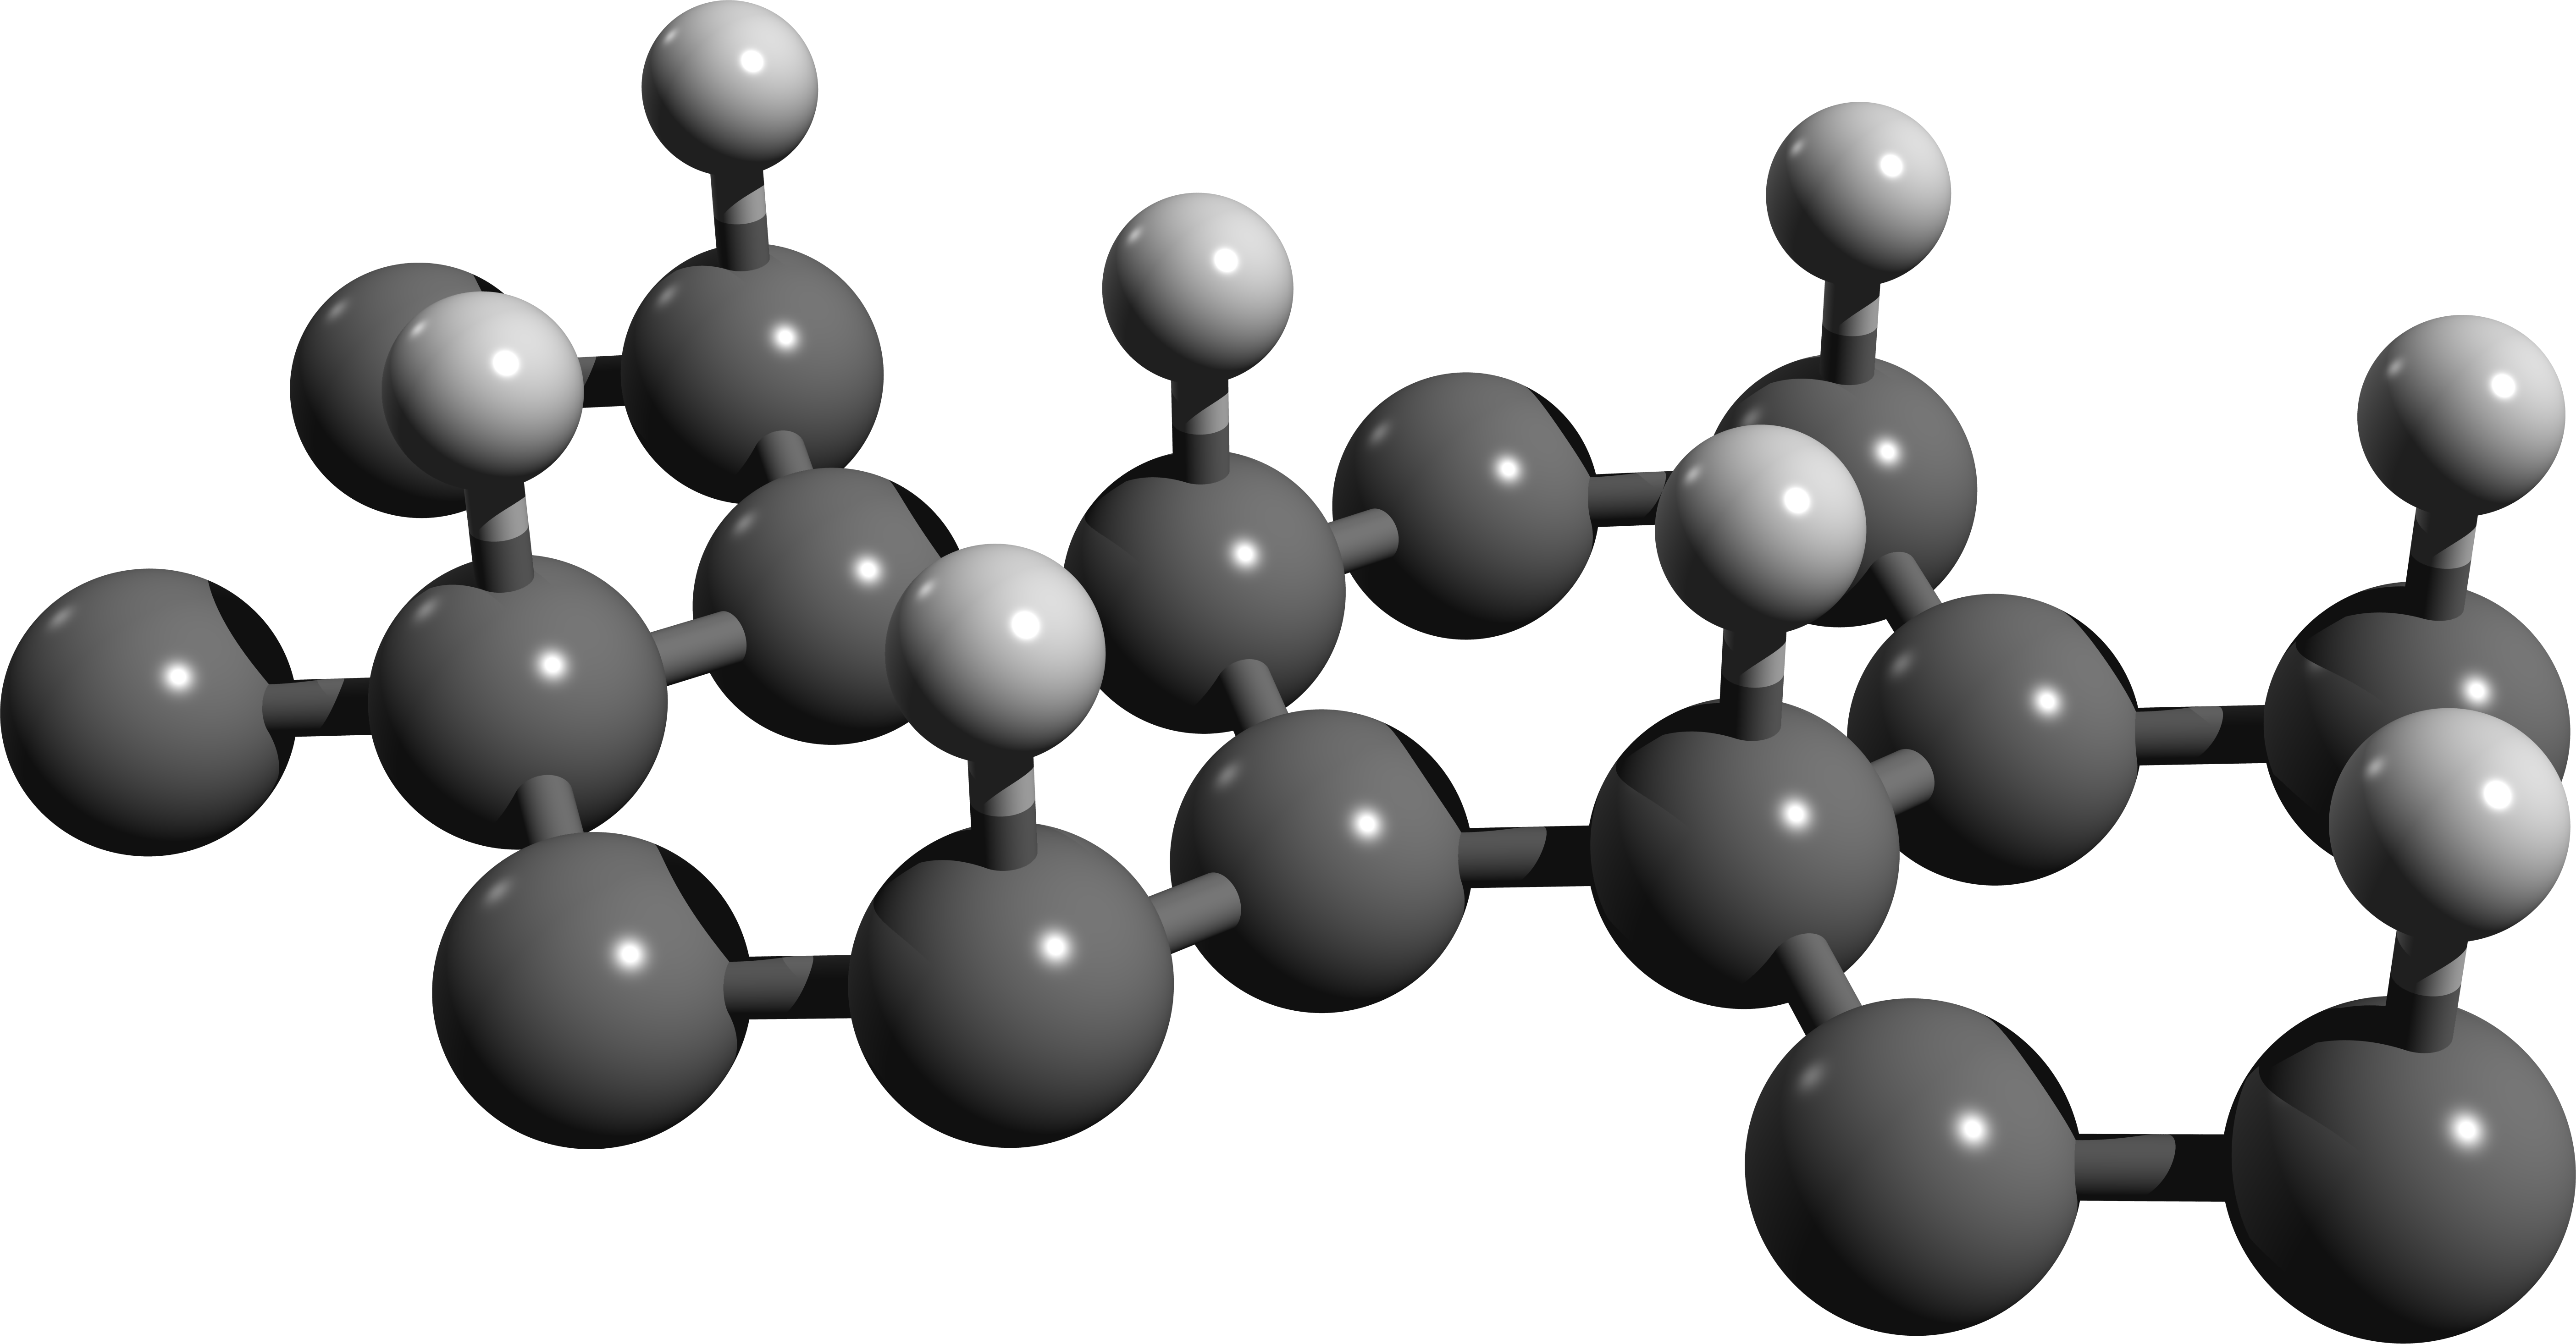
\includegraphics[width=1.0\textwidth]{figs/up3.png}};

\node[anchor=south west,inner sep=0] at (0.6,-0.3) 
{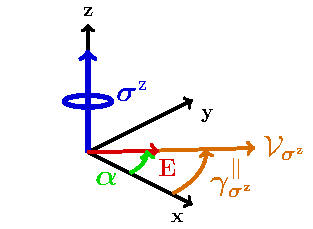
\includegraphics[width=0.85\textwidth]{figs/coord3.pdf}};

\end{tikzpicture}
\end{figure}

\vspace{-9mm}

\begin{figure}[h!]
\begin{tikzpicture}

\node[anchor=south west,inner sep=0,opacity=0.40] at (0.2,-0.3) 
{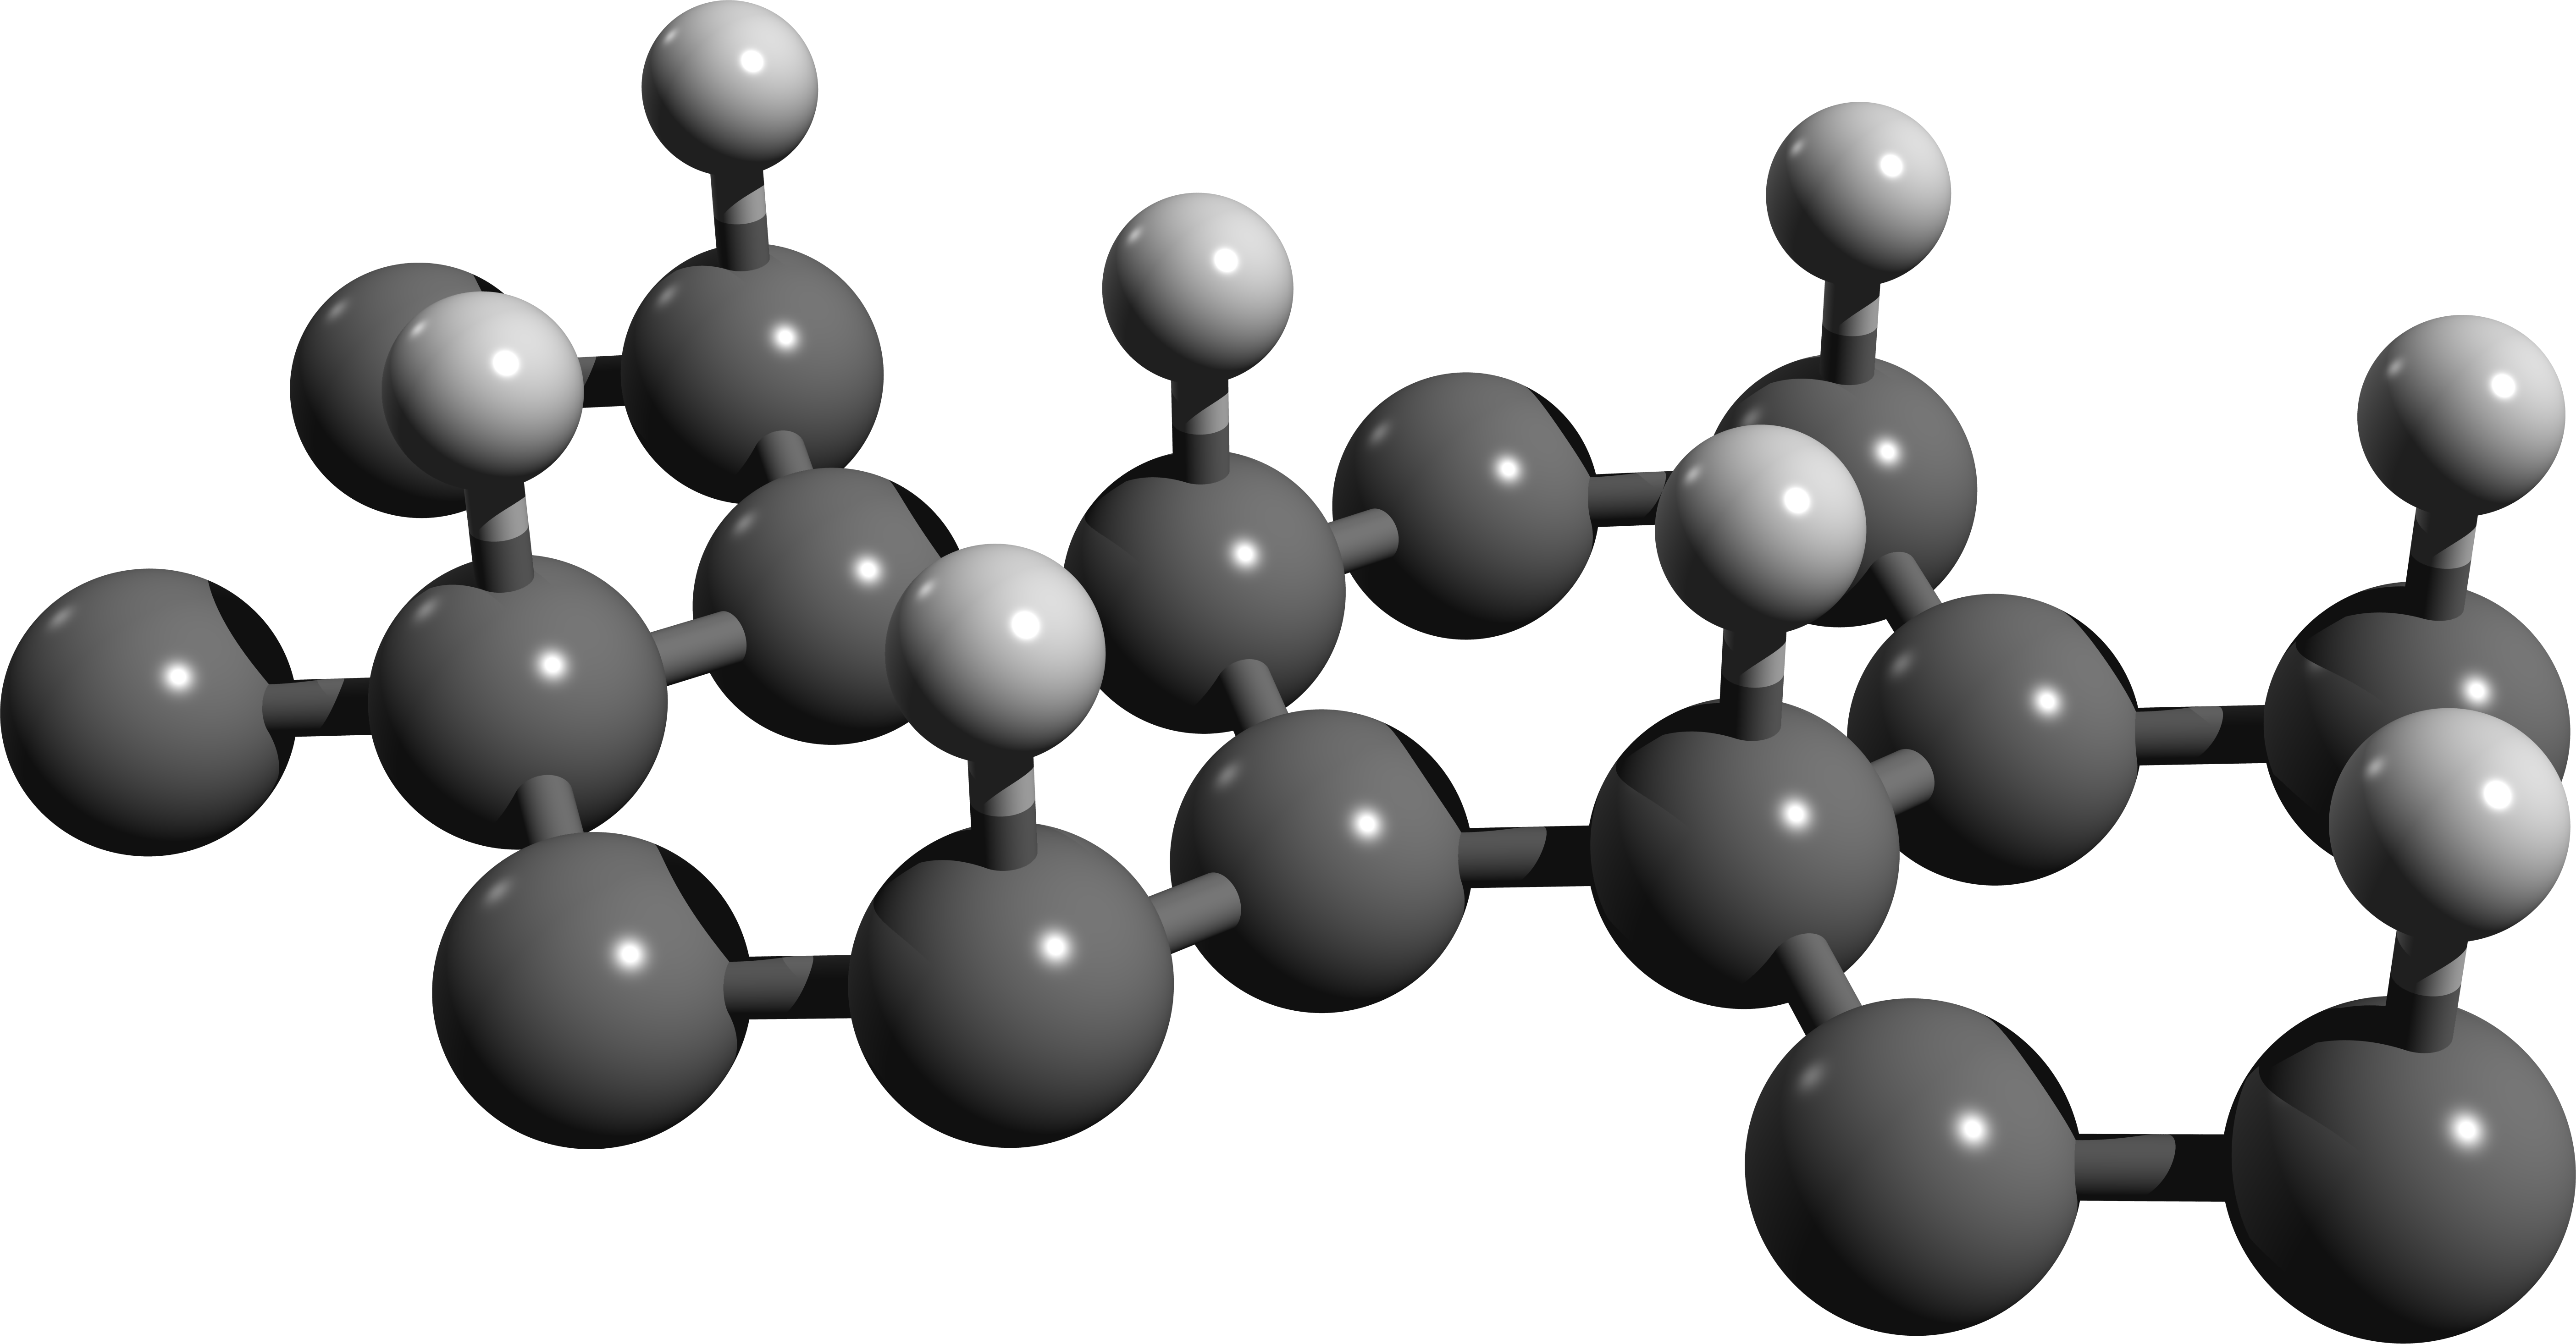
\includegraphics[width=1.0\textwidth]{figs/up3.png}};

\node[anchor=south west,inner sep=0] at (0.2,-0.6) 
{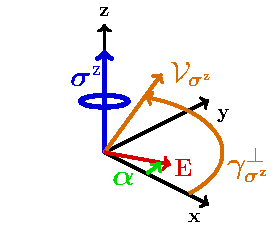
\includegraphics[width=0.85\textwidth]{figs/coord4.pdf}};

\end{tikzpicture}
\end{figure}


\end{columns}

}

\end{frame}

%%%%%%%%%%%%%%%%%%%%%%%%%%%%%%%%%%%%%%%%%%%%%%%%%%%%%%%%%%%%%%%%%%%%%%%%%%%%%

%%%%%%%%%%%%%%%%%%%%%%%
\subsection{Fixing the spin velocity}
%%%%%%%%%%%%%%%%%%%%%%%

\begin{frame}

{\Large Fixing the spin velocity\footnote[frame]
{\tiny Reinaldo Zapata-Pe\~na et. al. Phys. Rev. B 96, 195415. 2017}}


{\small

\begin{columns}

\column{0.55\textwidth}

\vspace{-5mm}

\begin{center}
{\large Velocity fixed along $y$ direction}
\end{center}

\vspace{-9mm}

\begin{figure}[h!]
\begin{tikzpicture}


\node[anchor=south west,inner sep=0,opacity=0.40] at (0.2,-0.3) 
{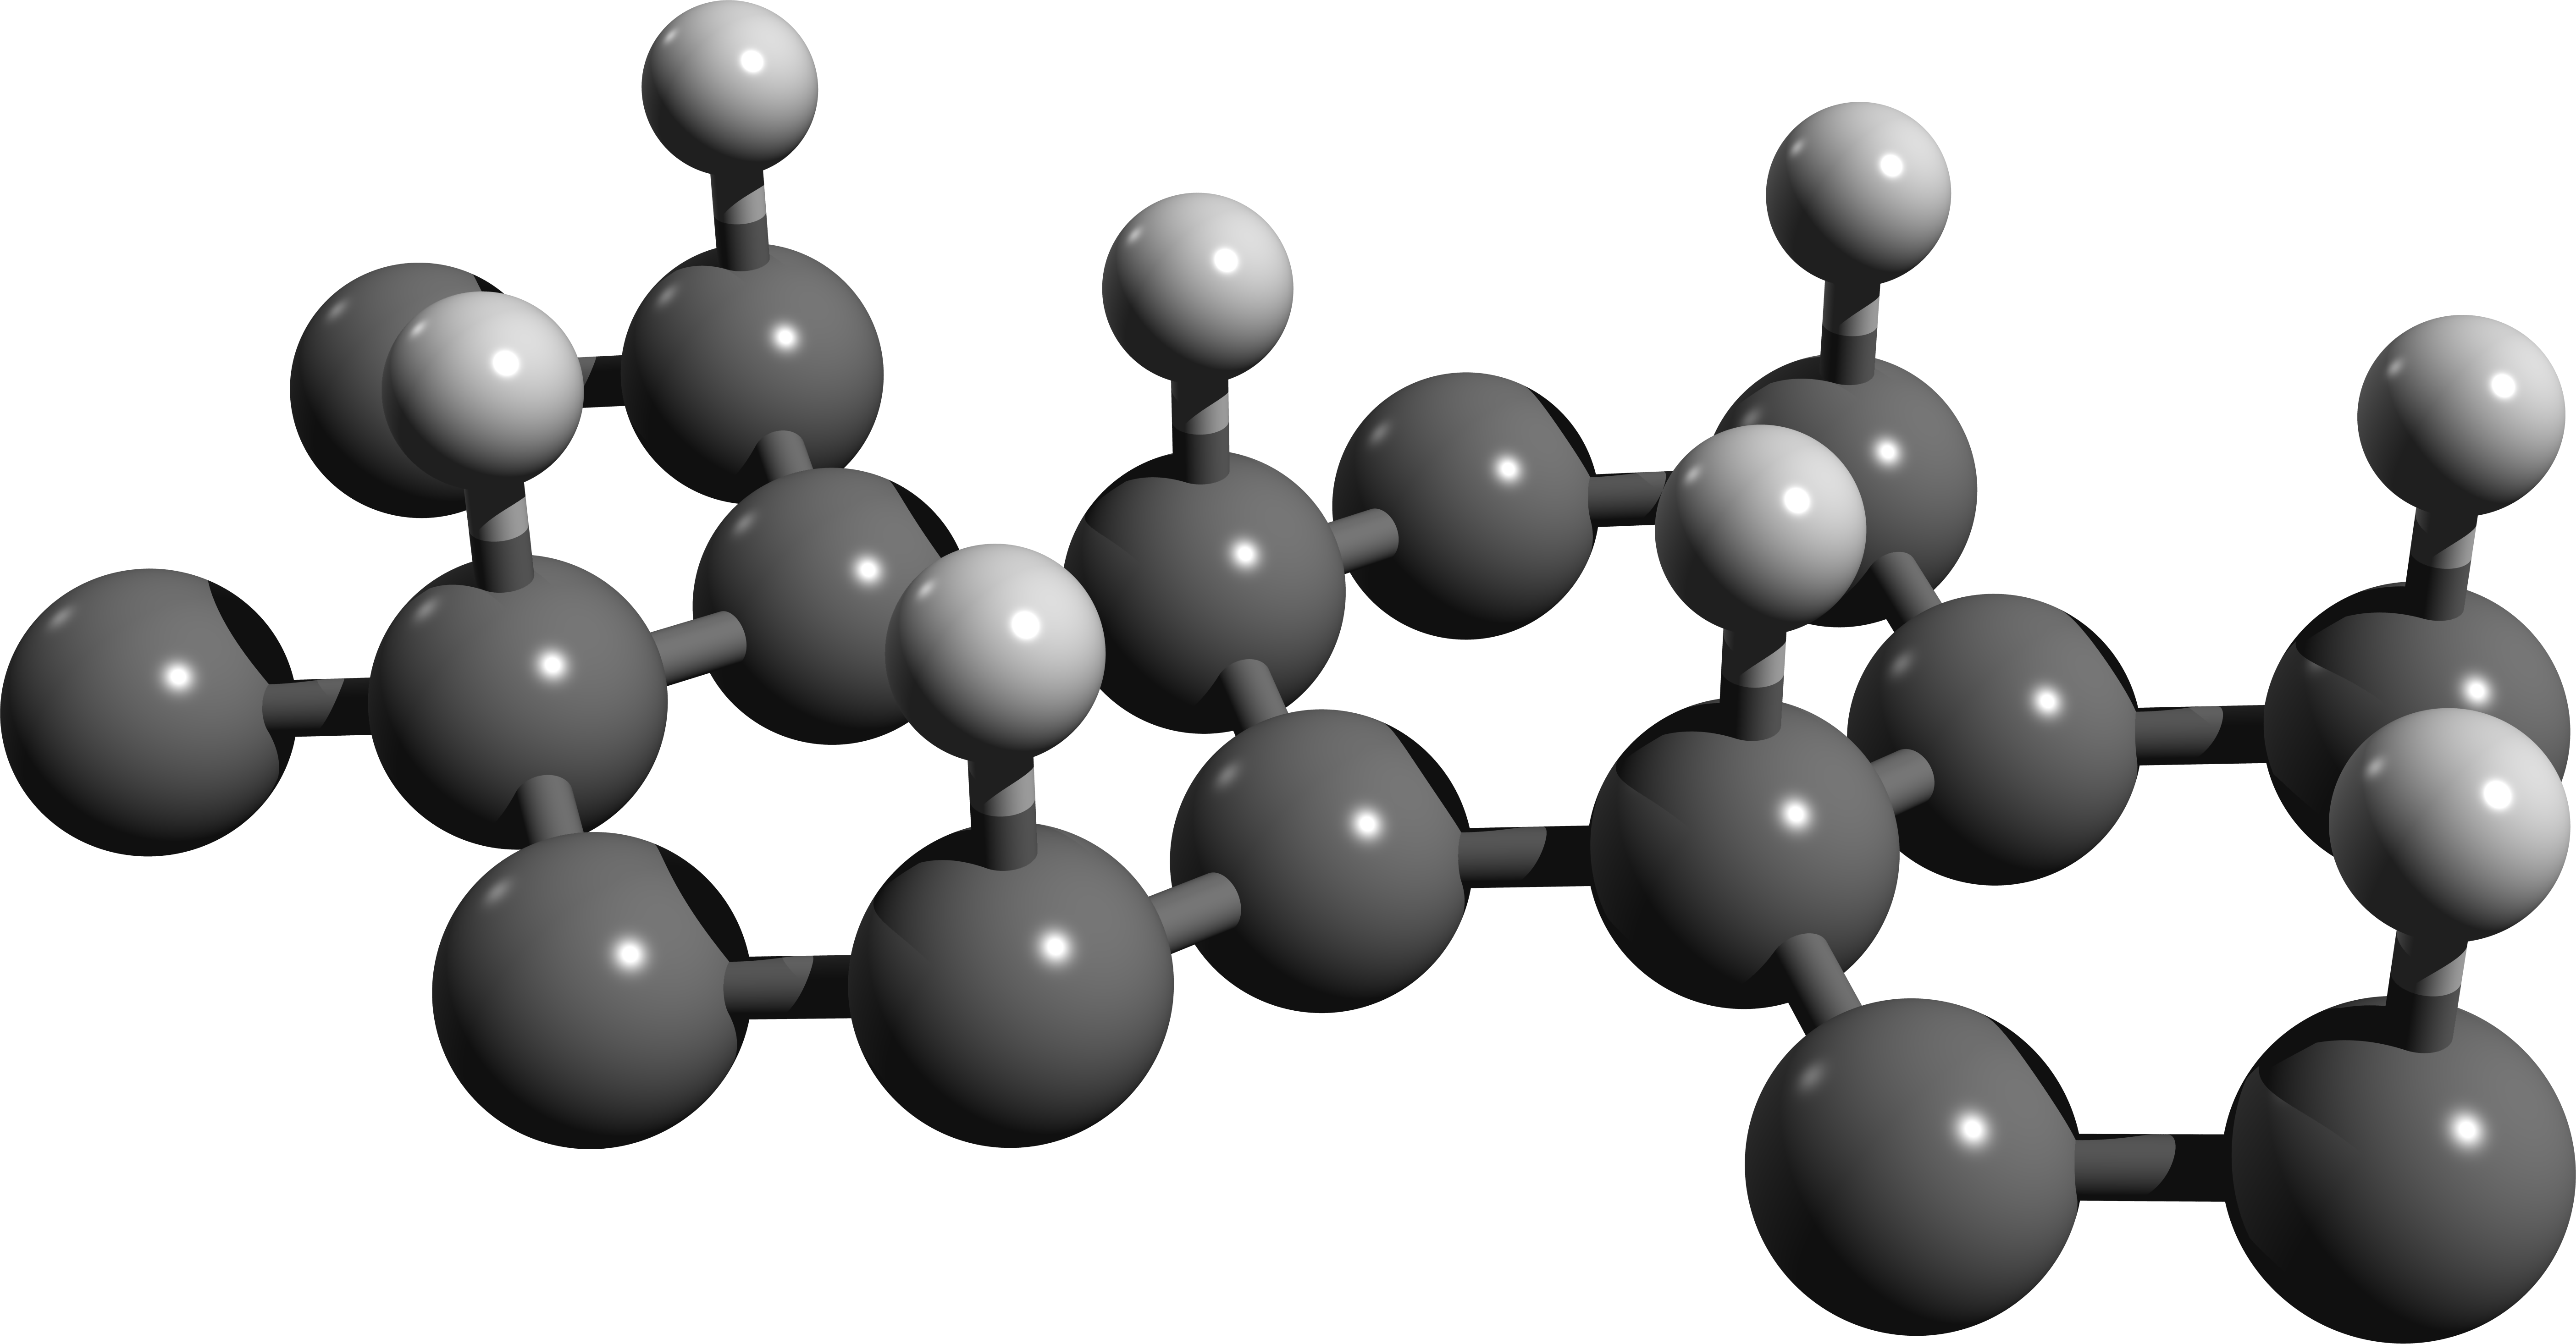
\includegraphics[width=1.0\textwidth]{figs/up3.png}};

\node[anchor=south west,inner sep=0] at (0.1,-0.7) 
{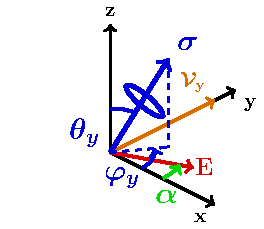
\includegraphics[width=0.85\textwidth]{figs/coord5.pdf}};

\end{tikzpicture}
\end{figure}

\column{0.5\textwidth}

\begin{itemize}

\item Magnitude of the velocity when it is fixed along $\mathbf{\hat{a}}$
direction
\vspace{-2mm}
\begin{align}
\mathcal{V}&_{\mathrm{a}}(\omega,\alpha) \equiv 
\left[
\left(\mathcal{V}^{\mathrm{ax}}(\omega,\alpha)\right)^{2} +
\right. \nonumber  \\ & \left.
\left(\mathcal{V}^{\mathrm{ay}}(\omega,\alpha)\right)^{2} +
\left(\mathcal{V}^{\mathrm{az}}(\omega,\alpha)\right)^{2} \right]
.
\label{eq:vv-mag}
\end{align}

\vspace{-5mm}

\item 
Angles of the spin

Polar angle
\vspace{-3mm}
\begin{equation}
\theta_{\mathrm{a}}  (\omega,\alpha) = 
\cos^{-1} \left( \frac{\mathcal{V}^{\mathrm{az}}(\omega,\alpha)}
{\mathcal{V}_{\mathrm{a}}(\omega,\alpha)} \right).
\label{eq:polar-ang}
\end{equation}

\vspace{-2mm}
Azimuthal angle
\vspace{-3mm}
\begin{equation}
\varphi_{\mathrm{a}} (\omega,\alpha) =
\tan^{-1} \left( \frac{\mathcal{V}^{\mathrm{ay}}(\omega,\alpha)}
{\mathcal{V}^{\mathrm{ax}}(\omega,\alpha)} \right).
\label{eq:azimuthal-ang} 
\end{equation} 

\end{itemize}
\end{columns}

}

\end{frame}


%%%%%%%%%%%%%%%%%%%%%%%%%%%%%%%%%%%%%%%%%%%%%%%%%%%%%%%%%%%%%%%%%%%%%%%%%%%%%

%%%%%%%%%%%%%%%%%%%%%%%
\subsection{Optical current injection}
%%%%%%%%%%%%%%%%%%%%%%%


\begin{frame}


\vspace{-0.2cm}

\noindent\makebox[\linewidth]{\rule{\linewidth}{0.4pt}}

\vspace{-2.0mm}
\begin{center}
{\large Optical current injection}
\end{center}

\vspace{-6mm}
\noindent\makebox[\linewidth]{\rule{\linewidth}{0.4pt}}


{\small


\begin{columns}


\column{0.6\textwidth}

\vspace{-4mm}
\begin{figure}[h!]
\begin{tikzpicture}

\node[anchor=south west,inner sep=0] at (0.2,-0.3) 
{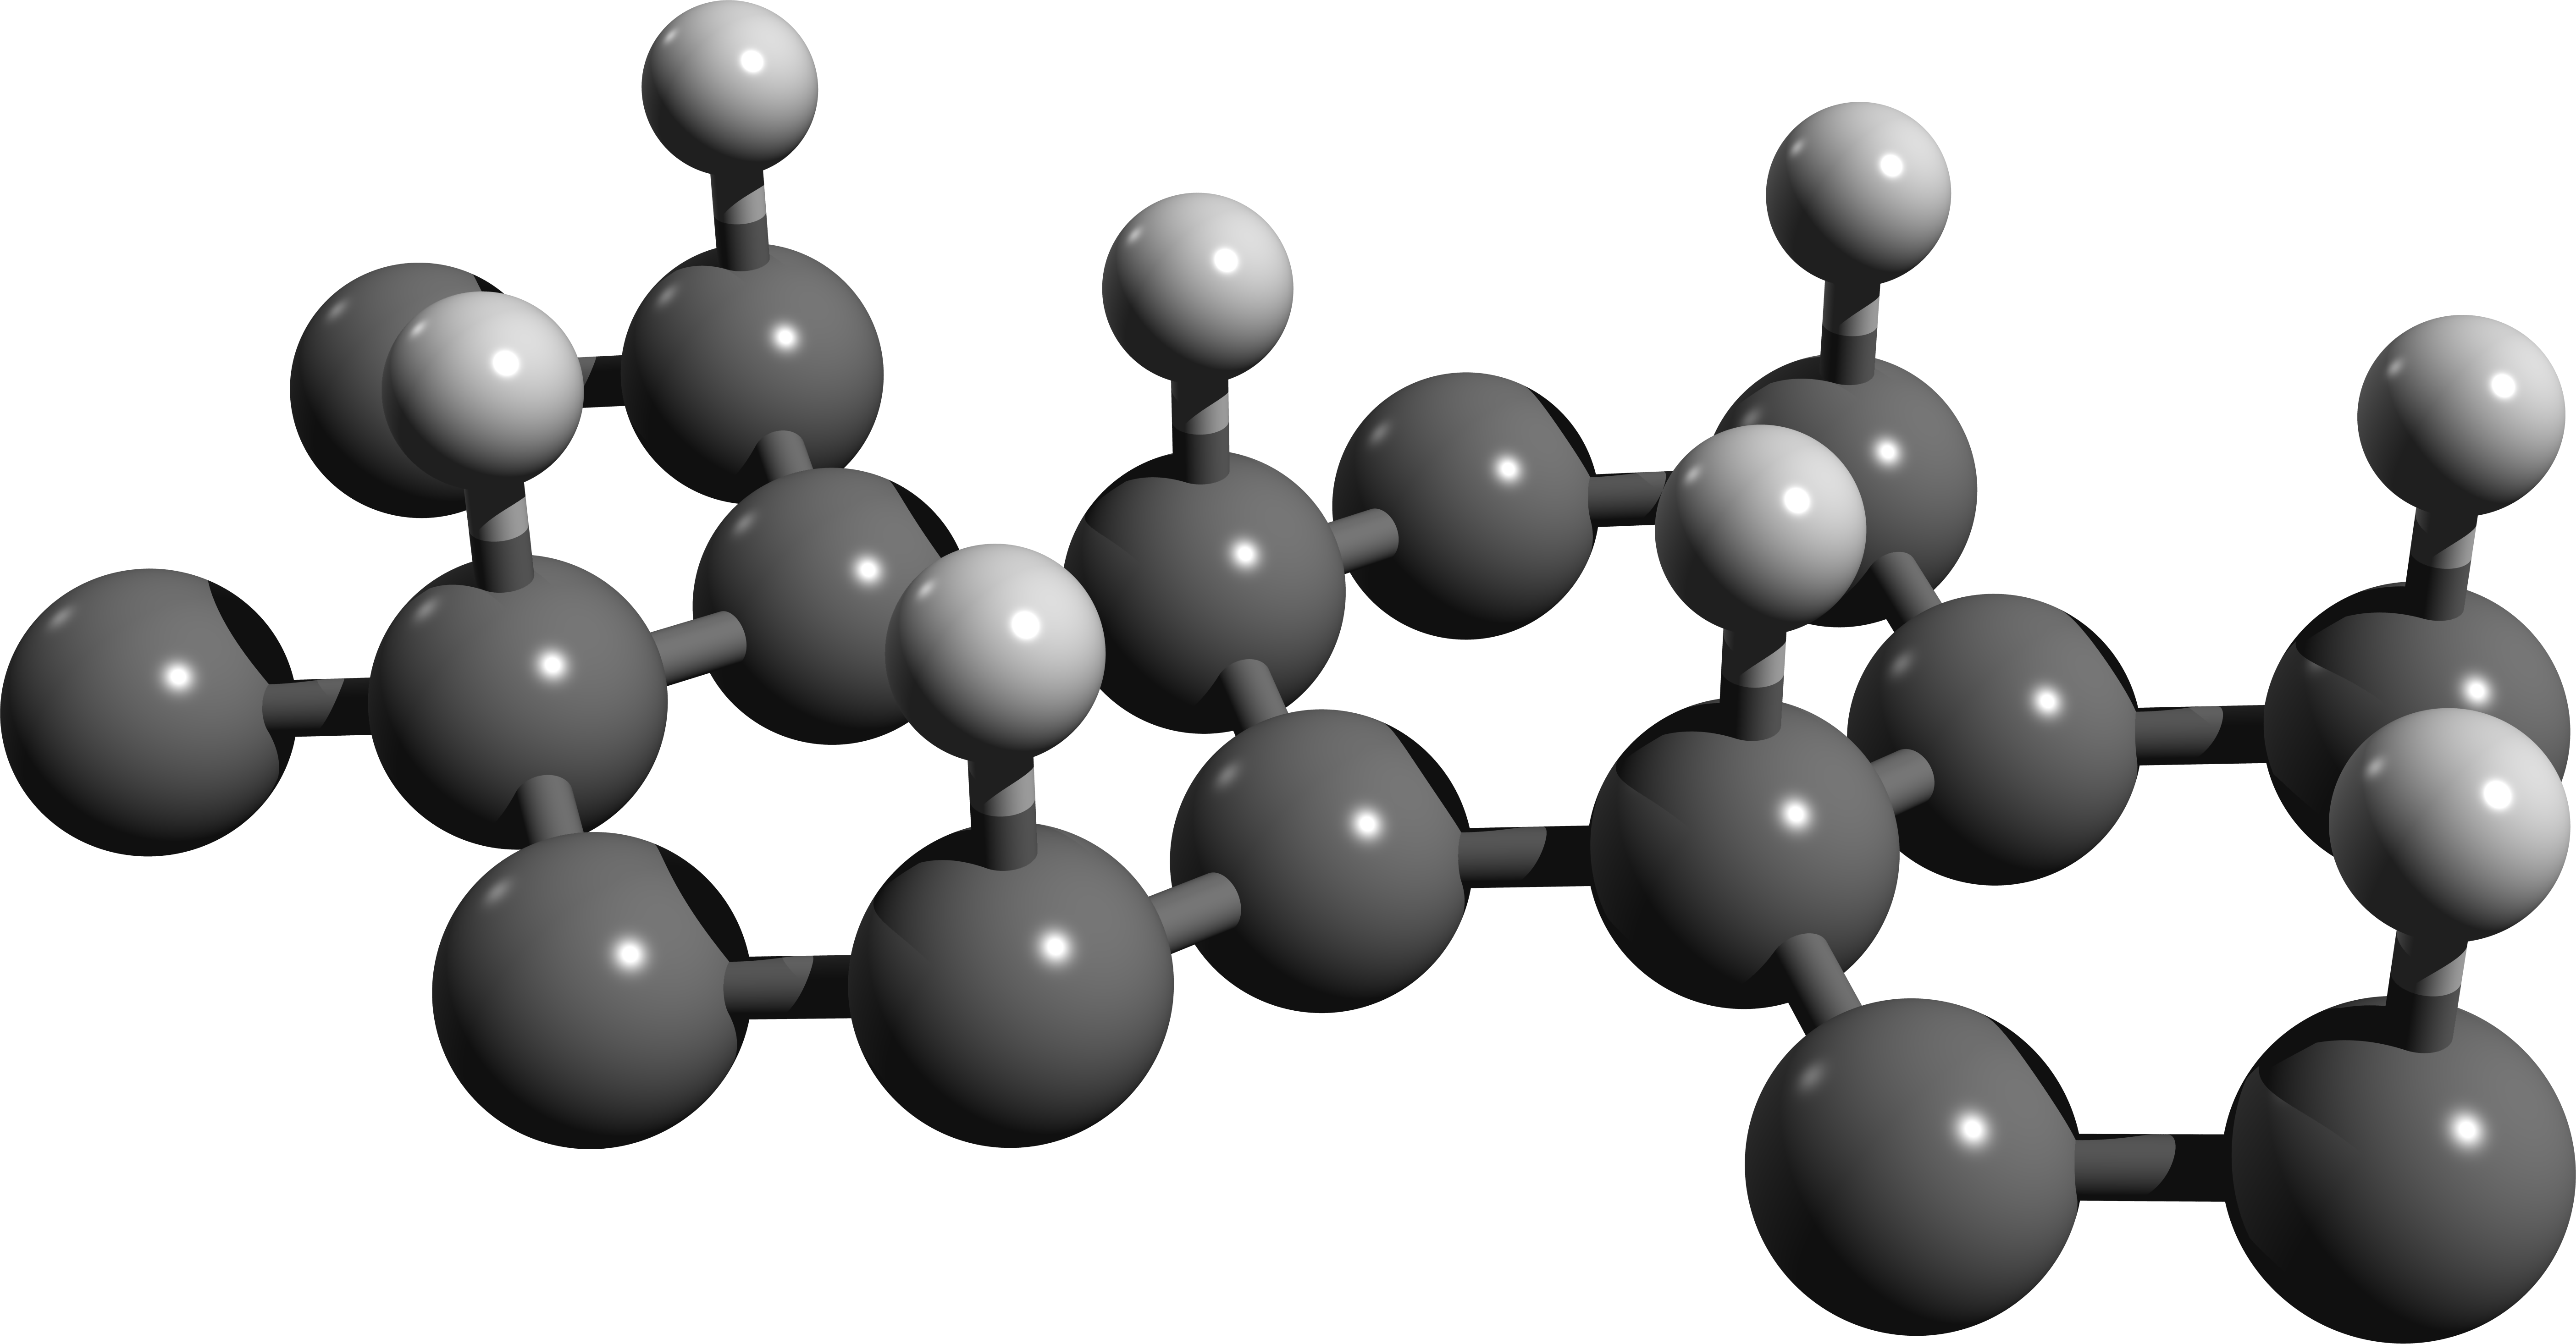
\includegraphics[width=1.0\textwidth]{figs/up3.png}};
\node[anchor=south west,inner sep=0] at (1.9, 0.0) 
{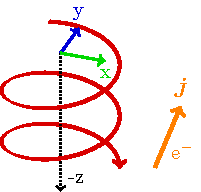
\includegraphics[width=0.7\textwidth]{figs/helix2.pdf}};

\end{tikzpicture}
\end{figure}


\column{0.4\textwidth}

\begin{itemize}

\item 
It is possible to control a photocurrent in a bulk structure 
\footnote[frame]{\tiny A. Hache\' et. al. Phys. Rev. Lett., 78:306-309, Jan
1997.}
or in the surface of a 2D system.
\footnote[frame]{\tiny N. Arzate et al. Phys. Rev. B, 90(20):205310, 2014.}
\hspace{-1mm}\textsuperscript{,}
\footnote[frame]{\tiny R. Zapata-Pe\~na et. al. Phys. Stat. Sol. (b), 253
(2):226-233, 2016.}

\item 
Is a second-order optical nonlinear effect that can be produced with a single
optical circularly-polarized beam.\textsuperscript{ 2}


\end{itemize}


\end{columns}


}

\end{frame}

%%%%%%%%%%%%%%%%%%%%%%%%%%%%%%%%%%%%%%%%%%%%%%%%%%%%%%%%%%%%%%%%%%%%%%%%%%%%%


\begin{frame}


{\small

\begin{itemize}

\item 
A photocurrent can be injected into noncentrosymmetric materials or at the
surface of bulk centrosymmetric materials and is given by
\footnote[frame]{\tiny N. Arzate et al. Phys. Rev. B, 90(20):205310, 2014.}
\begin{equation*}
\mathbf{\dot{J}}^{a}_{\text{inj}}(\omega) =
\eta^{abc}(\omega)E_{b}(\omega)E_{c}(\omega), \label{eq:current}
\end{equation*}
where $\eta^{abc}(\omega)$ is the current injection tensor which quantifies the
current injection along the a direction $a$.

\item The response was calculated layer by layer.


\end{itemize}
}
\end{frame}

%%%%%%%%%%%%%%%%%%%%%%%%%%%%%%%%%%%%%%%%%%%%%%%%%%%%%%%%%%%%%%%%%%%%%%%%%%%%%



%%%%%%%%%%%%%%%%%%%%%%%
\subsection{Second harmonic generation}
%%%%%%%%%%%%%%%%%%%%%%%


\begin{frame}

\vspace{-0.2cm}

\noindent\makebox[\linewidth]{\rule{\linewidth}{0.4pt}}

\vspace{-2.0mm}
\begin{center}
{\large Second harmonic generation (SHG)}
\end{center}

\vspace{-6mm}
\noindent\makebox[\linewidth]{\rule{\linewidth}{0.4pt}}



\begin{columns}

\column{0.40\textwidth}

{\small


\begin{itemize}

\item 
Is a second-order optical nonlinear effect and a particular case of sum
frequency generation.

\item 
The nonlinear polarization in the media acts as a source for the
electromagnetic waves of frequency $2\omega$.

\item 
SHG spectroscopy offer a non-invasive technique to study material properties.

\end{itemize}
}

\column{0.60\textwidth}

\begin{figure}[h!]
\begin{tikzpicture}

\node[anchor=south west,inner sep=0] at (0.2,-0.3) 
{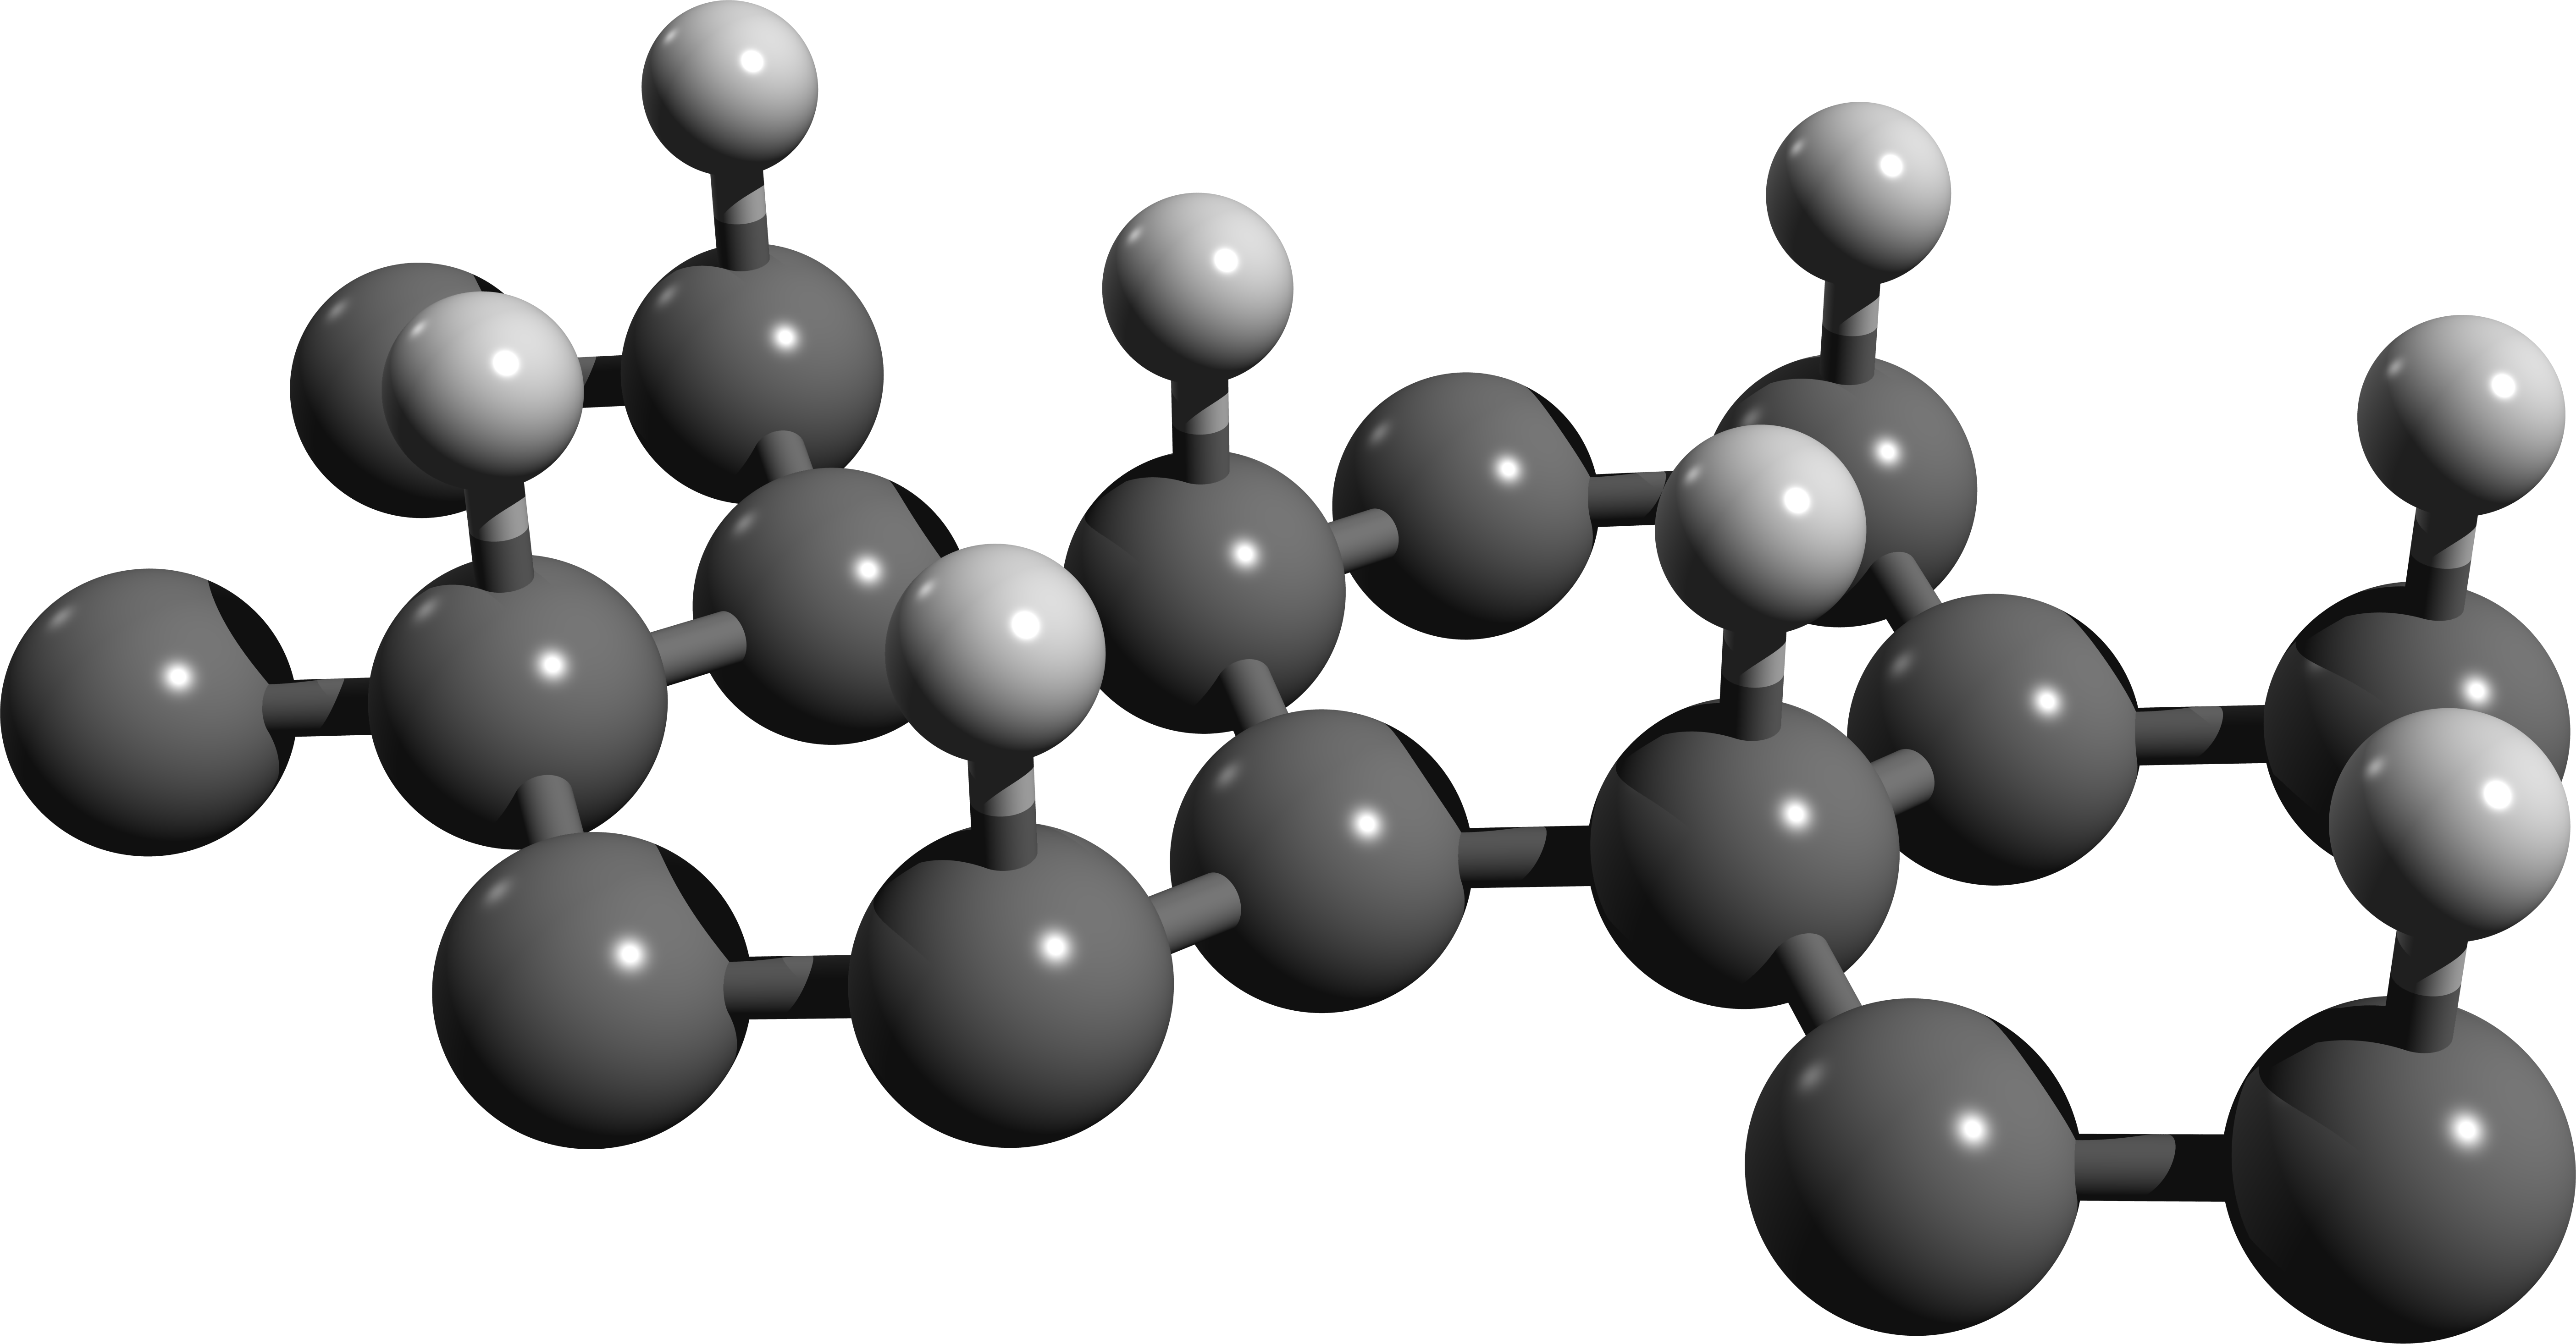
\includegraphics[width=1.0\textwidth]{figs/up3.png}};
\node[anchor=south west,inner sep=0] at (0.7, 0.8) 
{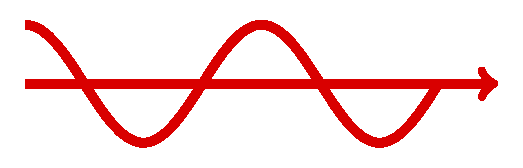
\includegraphics[width=0.55\textwidth,angle=-45,origin=c]
{figs/arrow_1omega.pdf}};
\node[anchor=south west,inner sep=0] at (3.0, 0.8) 
{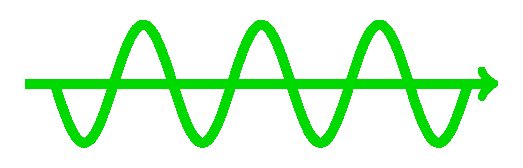
\includegraphics[width=0.55\textwidth,angle=45,origin=c]
{figs/arrow_2omega.pdf}};
\draw [] (1.00, 4.10) node [right] {\Large $\omega$};
\draw [] (5.40, 4.10) node [right] {\Large $2\omega$};
\end{tikzpicture}
\end{figure}


\end{columns}

\end{frame}

%%%%%%%%%%%%%%%%%%%%%%%%%%%%%%%%%%%%%%%%%%%%%%%%%%%%%%%%%%%%%%%%%%%%%%%%%%%%%

\begin{frame}


{\small

\begin{itemize}

\item 
The second-order nonlinear polarization is given by
\footnote[frame]{\tiny S. M. Anderson et al. Phys. Rev. B, 91(7):075302, 2015.}
\begin{equation*}\label{eq:pol}
\mathcal{P}(2\omega) = 
\chi^{abc}(-2\omega;\omega,\omega)E^{b}(\omega)E^{c}(\omega),
\end{equation*} 
where $\chi^{abc}(-2\omega;\omega,\omega)$ is the nonlinear susceptibility
tensor responsible for the SHG.

\item 
The formalism includes\textsuperscript{ 1}
\begin{itemize}
\item [$-$] the scissors correction,
\item [$-$] the contribution of the nonlocal part of the pseudopotentials
\item [$-$] the cut function used to select the individual contribution for
a given layer.
\end{itemize}

\end{itemize}
}
\end{frame}



%%%%%%%%%%%%%%%%%%%%%%%%%%%%%%%%%%%%%%%%%%%%%%%%%%%%%%%%%%%%%%%%%%%%%%%%%%%%%
\section{Results}
%%%%%%%%%%%%%%%%%%%%%%%%%%%%%%%%%%%%%%%%%%%%%%%%%%%%%%%%%%%%%%%%%%%%%%%%%%%%%



%%%%%%%%%%%%%%%%%%%%%%%
\subsection{Degree of spin polarization}
%%%%%%%%%%%%%%%%%%%%%%%


%%%%%%%%%%%%%%%%%%%%%%%%%%%%%%%%%%%%%%%%%%%%%%%%%%%%%%%%%%%%%%%%%%%%%%%%%%%%%


\begin{frame}

\begin{center}
{\Large Degree of spin polarization}
\end{center}

\begin{columns}

\column{0.52\textwidth}
\begin{center}
\small

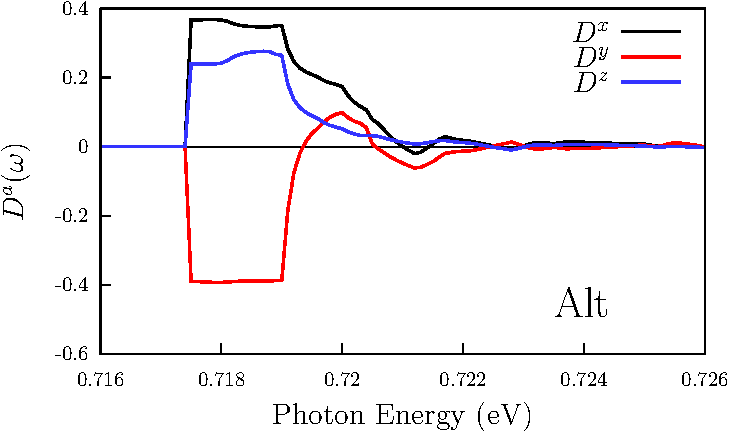
\includegraphics[width=0.99\textwidth]{figs/plots/dsp-alt.pdf}
\vspace{3mm}
\includegraphics[width=0.8\textwidth]{figs/alt2.png}

Response in the Near Infrared

0.717\,eV = 1.72\,$\mu$m = 173\,THz

\end{center}



\column{0.52\textwidth}
\begin{center}
\small 

\vspace{-1mm}
\includegraphics[width=1.0\textwidth]{figs/plots/dsp-up.pdf}
\vspace{6mm}
\includegraphics[width=0.7\textwidth]{figs/up2.png}

\vspace{7mm}
Response in the Mid Infrared

0.084\,eV = 14.7\,$\mu$m = 20.3\,THz

\end{center}


\end{columns}

\end{frame}


%%%%%%%%%%%%%%%%%%%%%%%
\subsection{Spin velocity injection}
%%%%%%%%%%%%%%%%%%%%%%%


\begin{frame}

{\small

{\Large Spin velocity injection}

\begin{columns}


\column{0.5\textwidth}

\begin{center}

\vspace{-10mm}

\begin{figure}[h!]
\begin{tikzpicture}


\node[anchor=south west,inner sep=0,opacity=0.40] at (0.2,-0.3) 
{\includegraphics[width=0.70\textwidth]{figs/up3.png}};

\node[anchor=south west,inner sep=0] at (0.75,-0.65) 
{\includegraphics[width=0.55\textwidth]{figs/coord6.pdf}};

\end{tikzpicture}
\end{figure}

\vspace{-10mm}

\begin{figure}[h!]
\begin{tikzpicture}


\node[anchor=south west,inner sep=0,opacity=0.40] at (0.2,-0.3) 
{\includegraphics[width=0.70\textwidth]{figs/alt3.png}};

\node[anchor=south west,inner sep=0] at (0.60,-0.45) 
{\includegraphics[width=0.55\textwidth]{figs/coord7.pdf}};

\end{tikzpicture}
\end{figure}

% \vspace{4mm}
\vspace{4mm}

Components with maximum values of the $\mathcal{V}^{\mathrm{ab}}$ for the
\emph{alt}, \emph{up}, CdSe and GaAs structures.


\end{center}

\column{0.55\textwidth}

\vspace{-5mm}

\includegraphics[width=0.98\textwidth]{figs/plots/fig3.pdf}

\end{columns}


}
\end{frame}

    
%%%%%%%%%%%%%%%%%%%%%%%%%%%%%%%%%%%%%%%%%%%%%%%%%%%%%%%%%%%%%%%%%%%%%%%%%%%%%


\begin{frame}

\begin{columns}

\column{0.65\textwidth}

\begin{center}

Fixing the spin along $z$ for \emph{up}

\vspace{2mm}

\includegraphics[width=0.95\textwidth]{figs/fig4.pdf}

\end{center}  

\column{0.42\textwidth}


{ When the spin is polarized along $z$ the spin velocity
$\mathcal{V}_{\sigma^{z}}$:}


\vspace{-2mm}

{\small

\begin{itemize}

\item 
Is maximized for $\hbar \omega = 0.084\,eV$

\vspace{-1mm}
\item 
The absolute maxima is 739.7\,Km/s for $\alpha = 35^{\circ}$

\vspace{-1mm}
\item 
The velocity is directed almost at a constant angle $\gamma_{\sigma^{z}} =
64.5^
{\circ}$

\end{itemize}

}

\vspace{-6mm}
\begin{center}

\begin{figure}[h!]
\begin{tikzpicture}

\node[anchor=south west,inner sep=0,opacity=0.40] at (0.2,-0.3) 
{\includegraphics[width=1.00\textwidth]{figs/up3.png}};

\node[anchor=south west,inner sep=0] at (1.0,-0.45) 
{\includegraphics[width=0.75\textwidth]{figs/coord8.pdf}};

\end{tikzpicture}
\end{figure}


\end{center}


\end{columns}

\end{frame}

%%%%%%%%%%%%%%%%%%%%%%%%%%%%%%%%%%%%%%%%%%%%%%%%%%%%%%%%%%%%%%%%%%%%%%%%%%%%%


\begin{frame}

\begin{columns}

\column{0.42\textwidth}

{\small

\begin{itemize}

\item 
A local maxima is found for $\hbar \omega = 1.954$\,eV (634\,nm, visible
red)

\item 
The maxima is 193.5\,Km/s for $\alpha = 35^{\circ}$

\item 
The velocity angle $\gamma_{\sigma^{z}}$ has values between $75.5^{\circ}$
and $77.8^{\circ}$

\end{itemize}

}

\vspace{-6mm}
\begin{center}

\begin{figure}[h!]
\begin{tikzpicture}

\node[anchor=south west,inner sep=0,opacity=0.40] at (0.2,-0.3) 
{\includegraphics[width=1.00\textwidth]{figs/up3.png}};

\node[anchor=south west,inner sep=0] at (1.0,-0.45) 
{\includegraphics[width=0.75\textwidth]{figs/coord9.pdf}};

\end{tikzpicture}
\end{figure}


\end{center}

\column{0.65\textwidth}

\begin{center}

Fixing the spin along $z$ for \emph{up}

\vspace{2mm}

\includegraphics[width=0.95\textwidth]{figs/fig5.pdf}

\end{center}  


\end{columns}

\end{frame}

%%%%%%%%%%%%%%%%%%%%%%%%%%%%%%%%%%%%%%%%%%%%%%%%%%%%%%%%%%%%%%%%%%%%%%%%%%%%%


\begin{frame}

\begin{columns}

\column{0.65\textwidth}

\begin{center}

Fixing the spin along $z$ for \emph{alt}

\vspace{2mm}

\includegraphics[width=0.95\textwidth]{figs/fig6.pdf}

\end{center}  

\column{0.42\textwidth}


{ When the spin is polarized along $z$ the spin velocity
$\mathcal{V}_{\sigma^{z}}$:}


\vspace{-2mm}

{\small

\begin{itemize}

\item 
Is maximized for $\hbar \omega = 0.720$\,eV (near infrared, 1.72\,$\mu$m)

\vspace{-1mm}
\item 
The absolute maxima is 644.9\,Km/s for $\alpha = 150^{\circ}$

\vspace{-1mm}
\item 
The velocity angle $\gamma_{\sigma^{z}}$ has values from $108^{\circ}$ to 
$110^{\circ}$

\end{itemize}

}

\vspace{-9mm}
\begin{center}

\begin{figure}[h!]
\begin{tikzpicture}

\node[anchor=south west,inner sep=0,opacity=0.40] at (0.2,-0.3) 
{\includegraphics[width=1.00\textwidth]{figs/alt3.png}};

\node[anchor=south west,inner sep=0] at (1.0,-0.45) 
{\includegraphics[width=0.75\textwidth]{figs/coord10.pdf}};

\end{tikzpicture}
\end{figure}


\end{center}


\end{columns}

\end{frame}

%%%%%%%%%%%%%%%%%%%%%%%%%%%%%%%%%%%%%%%%%%%%%%%%%%%%%%%%%%%%%%%%%%%%%%%%%%%%%


\begin{frame}

\begin{columns}

\column{0.65\textwidth}

\begin{center}

\vspace{-3mm}
{\small Fixing the velocity on $x$ and $y$ directions for \emph{up}}

\vspace{2mm}

\includegraphics[width=0.80\textwidth]{figs/fig7.pdf}

\end{center}  

\column{0.42\textwidth}


\vspace{-2mm}


\vspace{-6mm}
\begin{center}

\begin{figure}[h!]
\begin{tikzpicture}
\hspace{-2mm}
\node[anchor=south west,inner sep=0,opacity=0.40] at (0.2,-0.3) 
{\includegraphics[width=1.00\textwidth]{figs/up3.png}};

\node[anchor=south west,inner sep=0] at (0.0,-0.25) 
{\includegraphics[width=0.50\textwidth]{figs/coord11.pdf}};

\node[anchor=south west,inner sep=0] at (2.5,-0.25) 
{\includegraphics[width=0.50\textwidth]{figs/coord12.pdf}};

\end{tikzpicture}
\end{figure}

{\small

\vspace{-2mm}
\begin{itemize}

\item The responses are maximized for $\alpha = 35^{\circ}$ and $\hbar \omega =
0.084$\,eV
\item The absolute $x$ maxima is 
$\mathcal{V}_{\mathrm{x}} = 431.7$\,Km/s at
$\theta_{\mathrm{x}} = 42.5^{\circ}$ and
$\varphi_{\mathrm{x}} = 208.3^{\circ}$

\item The absolute $y$ maxima is 
$\mathcal{V}_{\mathrm{y}} = 687.9$\,Km/s at 
$\theta_{\mathrm{y}} =13.9^{\circ}$ and
$\varphi_{\mathrm{y}} = 82.1^{\circ}$

\end{itemize}

}


\end{center}


\end{columns}

\end{frame}

%%%%%%%%%%%%%%%%%%%%%%%%%%%%%%%%%%%%%%%%%%%%%%%%%%%%%%%%%%%%%%%%%%%%%%%%%%%%%

\begin{frame}

\begin{columns}

\column{0.42\textwidth}

{\small

\vspace{-2mm}
\begin{itemize}

\item The responses has a local maxima for $\alpha = 35^{\circ}$ and $\hbar
\omega = 0.084$\,eV

\item The local $x$ maxima is 
$\mathcal{V}_{\mathrm{x}} = 61.2$\,Km/s at
$\theta_{\mathrm{x}} = 48.3^{\circ}$ and
$\varphi_{\mathrm{x}} = 54.3^{\circ}$

\item The local $y$ maxima is 
$\mathcal{V}_{\mathrm{y}} = 293.2$\,Km/s at 
$\theta_{\mathrm{y}} =49.8^{\circ}$ and
$\varphi_{\mathrm{y}} = 51.9^{\circ}$

\end{itemize}

}

\begin{center}

\vspace{-8mm}
\begin{figure}[h!]
\begin{tikzpicture}

\node[anchor=south west,inner sep=0,opacity=0.40] at (0.2,-0.3) 
{\includegraphics[width=1.00\textwidth]{figs/up3.png}};

\node[anchor=south west,inner sep=0] at (0.0,-0.25) 
{\includegraphics[width=0.50\textwidth]{figs/coord13.pdf}};

\node[anchor=south west,inner sep=0] at (2.5,-0.25) 
{\includegraphics[width=0.50\textwidth]{figs/coord14.pdf}};

\end{tikzpicture}
\end{figure}

\end{center}

\column{0.65\textwidth}

\begin{center}

\vspace{-6mm}

\includegraphics[width=0.80\textwidth]{figs/fig8.pdf}

\end{center}  

\end{columns}

\end{frame}

%%%%%%%%%%%%%%%%%%%%%%%%%%%%%%%%%%%%%%%%%%%%%%%%%%%%%%%%%%%%%%%%%%%%%%%%%%%%%

%%%%%%%%%%%%%%%%%%%%%%%%%%%%%%%%%%%%%%%%%%%%%%%%%%%%%%%%%%%%%%%%%%%%%%%%%%%%%

\begin{frame}

\begin{columns}

\column{0.65\textwidth}

\vspace{-3mm}

{\small Fixing the velocity on $x$ and $y$ directions for \emph{alt}}

\vspace{2mm}

\begin{center}

\vspace{-6mm}

\includegraphics[width=0.80\textwidth]{figs/fig9.pdf}

\end{center}  

\column{0.42\textwidth}

{\small

\vspace{-2mm}
\begin{itemize}

\item The responses has a local maxima for $\alpha = 150^{\circ}$ and $\hbar
\omega = 0.720$\,eV

\item The local $x$ maxima is 
$\mathcal{V}_{\mathrm{x}} = 301.7 $\,Km/s at
$\theta_{\mathrm{x}} = 44.5^{\circ}$ and
$\varphi_{\mathrm{x}} = 51.2^{\circ}$

\item The absolute $y$ maxima is 
$\mathcal{V}_{\mathrm{y}} = 905.6$\,Km/s at 
$\theta_{\mathrm{y}} = 119.7^{\circ}$ and
$\varphi_{\mathrm{y}} = 163.4^{\circ}$

\end{itemize}

}

\begin{center}

\vspace{-8mm}
\begin{figure}[h!]
\begin{tikzpicture}

\node[anchor=south west,inner sep=0,opacity=0.40] at (0.2,-0.3) 
{\includegraphics[width=1.00\textwidth]{figs/alt3.png}};

\node[anchor=south west,inner sep=0] at (0.0,-0.25) 
{\includegraphics[width=0.50\textwidth]{figs/coord15.pdf}};

\node[anchor=south west,inner sep=0] at (2.5,-0.22) 
{\includegraphics[width=0.50\textwidth]{figs/coord16.pdf}};

\end{tikzpicture}
\end{figure}

\end{center}

\end{columns}

\end{frame}

%%%%%%%%%%%%%%%%%%%%%%%%%%%%%%%%%%%%%%%%%%%%%%%%%%%%%%%%%%%%%%%%%%%%%%%%%%%%%

%%%%%%%%%%%%%%%%%%%%%%%
\subsection{optical current injection}
%%%%%%%%%%%%%%%%%%%%%%%

%%%%%%%%%%%%%%%%%%%%%%%%%%%%%%%%%%%%%%%%%%%%%%%%%%%%%%%%%%%%%%%%%%%%%%%%%%%%%

\begin{frame}

\begin{center}
{\Large Optical current injection}
\end{center}

\begin{columns}

\column{0.52\textwidth}
\begin{center}
\small

\includegraphics[width=0.99\textwidth]{figs/plots/eta-alt_y.pdf}
\vspace{3mm}
\includegraphics[width=0.8\textwidth]{figs/alt2.png}

Intense response in the Near Infrared

0.95\,eV = 230\,$\mu$m

\end{center}

\column{0.52\textwidth}
\begin{center}
\small 

\vspace{-1mm}
\includegraphics[width=1.0\textwidth]{figs/plots/eta-up_y.pdf}
\vspace{6mm}
\includegraphics[width=0.7\textwidth]{figs/up2.png}

\vspace{7mm}
Response in the Mid Infrared

0.084\,eV = 14.7\,$\mu$m = 20.3\,THz

\end{center}


\end{columns}

\end{frame}

%%%%%%%%%%%%%%%%%%%%%%%%%%%%%%%%%%%%%%%%%%%%%%%%%%%%%%%%%%%%%%%%%%%%%%%%%%%%%


%%%%%%%%%%%%%%%%%%%%%%%
\subsection{Second harmonic generation}
%%%%%%%%%%%%%%%%%%%%%%%

\begin{frame}

\begin{center}
{\Large Optical current injection}
\end{center}

\begin{columns}

\column{0.52\textwidth}
\begin{center}
\small

\includegraphics[width=0.99\textwidth]{figs/plots/shg-lay-alt.pdf}
\vspace{3mm}
\includegraphics[width=0.8\textwidth]{figs/alt2.png}

Intense response in the Near Infrared

0.95\,eV = 230\,$\mu$m

\end{center}

\column{0.52\textwidth}
\begin{center}
\small 

\vspace{-1mm}
\includegraphics[width=1.0\textwidth]{figs/plots/shg-lay-up.pdf}
\vspace{6mm}
\includegraphics[width=0.7\textwidth]{figs/up2.png}

\vspace{7mm}
Response in the Mid Infrared

0.084\,eV = 14.7\,$\mu$m = 20.3\,THz

\end{center}


\end{columns}

\end{frame}


%%%%%%%%%%%%%%%%%%%%%%%%%%%%%%%%%%%%%%%%%%%%%%%%%%%%%%%%%%%%%%%%%%%%%%%%%%%%%
\section{Conclusions and perspectives} 
%%%%%%%%%%%%%%%%%%%%%%%%%%%%%%%%%%%%%%%%%%%%%%%%%%%%%%%%%%%%%%%%%%%%%%%%%%%%%



%%%%%%%%%%%%%%%%%%%%%%%
\subsection{Conclusions}
%%%%%%%%%%%%%%%%%%%%%%%

%%%%%%%%%%%%%%%%%%%%%%%%%%%%%%%%%%%%%%%%%%%%%%%%%%%%%%%%%%%%%%%%%%%%%%%%%%%%%


\begin{frame}


{\Large Conclusions}
{\small

\begin{itemize}

\item 
Due to the fact that both structures are high non-centrosymmetric materials,
then it is possible to induced high intensity nonlinear responses in them.

\item 
Both structures are excellent candidates for spintronics applications:

\begin{itemize}
\item[$\boldsymbol{\ast}$] 
We found that the \emph{up} is more spin--polarizable than the \emph{alt} but
both reaches more than 50\% of DSP.

\item[$\boldsymbol{\ast}$] 
It is possible to generate pure-spin currents in our structures; also it is
possible to control the spin orientation or the current direction making
variations in the angle of the polarization of the incoming beam.

\item[$\boldsymbol{\ast}$] 
The spin velocities reached in the structures are usable for spintronics
devices.

\end{itemize}

\item 
The \emph{up} structure can achieve a large injection current being the
response bigger than most of other structures. \footnote[frame]{\tiny R.
Zapata-Pe\~na, \emph{et. al.} Phys. Rev. B 96, 195415, 2017.}

\item 
Both structures are excellent candidates to generate second harmonic,
particularly the \emph{up} one.


\end{itemize}
}

\end{frame}

%%%%%%%%%%%%%%%%%%%%%%%%%%%%%%%%%%%%%%%%%%%%%%%%%%%%%%%%%%%%%%%%%%%%%%%%%%%%%


%%%%%%%%%%%%%%%%%%%%%%%
\subsection{Articles, conferences and courses}
%%%%%%%%%%%%%%%%%%%%%%%


%%%%%%%%%%%%%%%%%%%%%%%%%%%%%%%%%%%%%%%%%%%%%%%%%%%%%%%%%%%%%%%%%%%%%%%%%%%%%

\begin{frame}
    
\begin{columns}

\column{0.5\textwidth}

{\Large Articles}

{\small
\begin{itemize}

\vspace{-2mm}
\item 
R. Zapata-Pe\~na, \emph{et. al.} Pure spin current injection in hydrogenated
   graphene structures. Phys. Rev. B 96, 195415, 2017.

\vspace{-2mm}
\item 
Anatoli I. Shkrebtii, R. Zapata-Pe\~na, \emph{et. al.} Graphene-Boron Nitride
   2D Heterosystems Functionalized with Hydrogen. Advances in Science and
   Technology 98:117-124, 2017.

\vspace{-2mm}
\item 
R. Zapata-Pe\~na, \emph{et. al.} Nonlinear optical responses in hydrogenated
   graphene structures. Phys. Stat. Sol. (b), 253(2):226-233, 2016.

\end{itemize}

}

\column{0.5\textwidth}

\includegraphics[width=1.0\textwidth]{figs/cover.pdf}

\end{columns}

\end{frame}


%%%%%%%%%%%%%%%%%%%%%%%%%%%%%%%%%%%%%%%%%%%%%%%%%%%%%%%%%%%%%%%%%%%%%%%%%%%%%


\begin{frame}

{\Large Conferences}

\begin{itemize}

\item OSI-11 2015 (Poster)
\item IX Riao-Optilas 2016 (Poster)

\end{itemize}

\vspace{7mm}

{\Large Specialized courses}

\begin{itemize}

\item Control de versiones usando Git y GitHub (2013)
\item C\'omputo en paralelo mediante FORTRAN/C++ con MPI y OpenMP (2013)
\item C\'alculo de propiedades o\'opticas de la materia con el uso de teor\'ia
de muchos cuerpos (2013)

\end{itemize}


\end{frame}


%%%%%%%%%%%%%%%%%%%%%%%%%%%%%%%%%%%%%%%%%%%%%%%%%%%%%%%%%%%%%%%%%%%%%%%%%%%%%


%%%%%%%%%%%%%%%%%%%%%%%
\subsection{Conclusions}
%%%%%%%%%%%%%%%%%%%%%%%


%%%%%%%%%%%%%%%%%%%%%%%%%%%%%%%%%%%%%%%%%%%%%%%%%%%%%%%%%%%%%%%%%%%%%%%%%%%%%



\begin{frame}

{\Large Perspectives}

\vspace{3mm}

Continue the study of this phenomenon in other structures and make new
publication:

\begin{columns}

\column{0.45\textwidth}

\begin{center}
\includegraphics[width=0.78\textwidth]{figs/hnbGh-aa-1.png}\\
\includegraphics[width=0.78\textwidth]{figs/hnbGh-ab-1.png}

Functionalized boron-nitride-graphene with hydrogen
\end{center}


\column{0.45\textwidth}


\begin{columns}

\vspace{-4mm}
\column{0.5\textwidth}

\includegraphics[width=1.0\textwidth]{figs/7-bnnt-1.png}

\column{0.5\textwidth}
\includegraphics[width=1.0\textwidth]{figs/7-bnnt-2.png}\\
\includegraphics[width=1.0\textwidth]{figs/7-bnnt-3.png}

\end{columns}

\begin{center}
Boron-nitride nanotubes
\end{center}


\end{columns}

\end{frame}


%%%%%%%%%%%%%%%%%%%%%%%%%%%%%%%%%%%%%%%%%%%%%%%%%%%%%%%%%%%%%%%%%%%%%%%%%%%%%
\section{Acknowledgments} 
%%%%%%%%%%%%%%%%%%%%%%%%%%%%%%%%%%%%%%%%%%%%%%%%%%%%%%%%%%%%%%%%%%%%%%%%%%%%%

\begin{frame}

\begin{center}
    
{\Large Acknowledgments}

\begin{itemize}
\item Dr. Bernardo Mendoza
\item Dr. Ram\'on Carriles Jaimes
\item Dr. Gabriel Merino Hern\'adez
\item My friend Dr. Sean M. Anderson
\item My wife, Patricia, and my kids 
\item My mother, Eloisa
\item My sisters
\item All my friends who shared time with me
\item The CIO
\item The CONACYT
\end{itemize}

\end{center}

\end{frame}



{
\usebackgroundtemplate{\includegraphics[height=\paperheight,width=\paperwidth]
{figs/end.jpg}}
\begin{frame}[plain]
\end{frame}
}







\end{document}


